\documentstyle[epic,eepic,graphicx,tabularx,tabulary,multirow,mathtools,cite,subfig,caption,appendix,algorithm,algorithmicx,algpseudocode,amssymb,listings,color,afterpage,placeins,url]{poly3}
%\mathindent 0pt

%%% Use includeonly to pdf only one chapter %%% <-------------------------------------------------------------------------------------------------------------
\includeonly{./chapters/introduction/introduction}

%\documentclass{report}[10pt]
%\usepackage{fancyhdr}
%\usepackage{amssymb}
%\usepackage{geometry}
%\usepackage{makecell}
%\usepackage[pdftex]{graphicx}
%\usepackage{mathtools}
%\usepackage{multicol}
%\usepackage[mathscr]{euscript}
%\usepackage[toc,page]{appendix}
%\usepackage[T1]{fontenc}
%\usepackage{titlesec, blindtext, color}
%\usepackage{framed}
%\usepackage{color}
%\usepackage{listings}
%\usepackage{dsfont}
%\usepackage{subcaption}
%\usepackage{natbib}
%\usepackage{tabularx}
%\usepackage[table]{xcolor}
%\usepackage{fullpage}
\newcolumntype{L}[1]{>{\hsize=#1\hsize\raggedright\arraybackslash}X}
\newcolumntype{R}[1]{>{\hsize=#1\hsize\raggedleft\arraybackslash}X}
\newcolumntype{C}[1]{>{\hsize=#1\hsize\centering\arraybackslash}X}

% Format Parameters
%\setlength{\parskip}{14pt plus 4pt minus 4pt}
%\linespread{1.125}

\newcommand{\col}[2]{\text{col}(#1)_{#2}}
\newcommand{\wrap}[1]{\left(#1\right)}
\newcommand{\sbrack}[1]{\left[#1\right]}
\newcommand{\setwrap}[1]{\left\{#1\right\}}
\newcommand{\abs}[1]{\left\lVert#1\right\rVert}
\newcommand{\norm}[1]{\left\lVert#1\right\rVert}
\newcommand{\ciel}[1]{\left\lceil#1\right\rceil}
%\definecolor{gray75}{gray}{0.75}

\newcommand{\mmathcal}[1]{{\cal #1}}
\newcommand{\mmathbb}[1]{{\Bbb #1}}

\newcommand{\Bellman}{T_{\gamma}^{\pi}}
\newcommand{\BellmanOpt}{T_{\gamma}^{*}}
\newcommand{\BellmanPiOpt}{T_{\gamma}^{\pi^{*}}}
\newcommand{\expect}[1]{\emph{E}\left[#1\right]}
\newcommand{\condexpect}[2]{\expect{#1 \middle\vert #2 }}
\newcommand{\expw}[1]{\exp\wrap*{#1}}
\newcommand{\Ssize}{\abs{S}}
\newcommand{\Asize}{\abs{A}}
\newcommand{\OptV}{V^{*}}
\newcommand{\Vpi}{V^{\pi}}
\newcommand{\OptPi}{\pi^{*}}
\newcommand{\OptVpi}{V^{\OptPi}}
\newcommand{\Aspace}{\mathcal{A}}
\newcommand{\Sspace}{\mathcal{S}}
\newcommand{\linedsection}[1]{\section*{#1}\vspace{-8mm}\hrulefill}
\newcommand{\hsp}{\hspace{20pt}}
\newcommand{\ith}{\hspace{0.1mm}$i^{th}$}
\newcommand{\jth}{\hspace{0.1mm}$j^{th}$}
\newcommand{\kth}{\hspace{0.1mm}$k^{th}$}
\newcommand{\Ith}{\hspace{0.1mm}$i^{th}$\hspace{0.5mm}}
\newcommand{\Jth}{\hspace{0.1mm}$j^{th}$\hspace{0.5mm}}
\newcommand{\Kth}{\hspace{0.1mm}$k^{th}$\hspace{0.5mm}}
\newcommand{\Forall}{\hspace{1mm}\forall\hspace{1mm}}
\newcommand{\SmallThenNormal}[1]{#1}
\newcommand{\RealVec}[1]{\in \emph{R}^{#1}}
\newcommand{\RealMat}[2]{\in \emph{R}^{#1\times#2}}
\newcommand{\Real}{\Re}
\newcommand{\RRe}{\mmathcal{R}}
\newcommand{\RRealVec}[1]{\in \RRe^{#1}}
\newcommand{\RRealMat}[2]{\in \RRe^{#1\times#2}}
\newcommand{\RReal}{\RRe}
\newcommand{\InRe}[1]{\in\RReal^{#1}}
\newcommand{\EqRef}[1]{Equation \ref{eq:#1}}
\newcommand{\EqLabel}[1]{\label{eq:#1}}
\newcommand{\FigRef}[1]{Figure \ref{fig:#1}}
\newcommand{\FigLabel}[1]{\label{fig:#1}}
\newcommand{\TableRef}[1]{Table \ref{tab:#1}}
\newcommand{\TableLabel}[1]{\label{tab:#1}}
\newcommand{\Sep}{\hspace{5mm}}
\newcommand{\SSep}{\hspace{2mm}}
\newcommand{\IE}{\emph{i.e.},\hspace{1mm}}
\newcommand{\EG}{\emph{e.g.},\hspace{1mm}}
\newcommand{\DotProd}[2]{\DotBrack*{#1,#2}}
\newcommand{\DiagMat}[1]{\text{diag}\wrap{#1}}
\newcommand{\Maps}[3]{ #1 \hspace{2mm} \Real^{#2} \rightarrow \Real^{#3}}
\newcommand{\Normalize}[1]{\frac{#1}{\norm{#1}}}
\newcommand{\Sig}[1]{\text{sig}\wrap{#1}}
\newcommand{\Unit}[1]{\emph{U}\wrap{#1}}
\newcommand{\Skew}[1]{\emph{S}\wrap{#1}}
\newcommand{\ForI}{ \forall i \in \SetWrap*{1,2,3,4} }
\newcommand{\Half}{0.5}
\newcommand{\Where} {\noindent where}
\newcommand{\SectionLabel}[1]{\label{sec:#1}}
\newcommand{\SectionRef}[1]{Section \ref{sec:#1}}
\newcommand{\SectionRefH}[1]{Section #1}
\newcommand{\SectionsRefH}[1]{Sections #1}
\newcommand{\SectionHead}[1]{\normalsize}
\newcommand{\SectionTail}[1]{\SectionLabel{#1}\normalsize}
\newcommand{\Project}[2]{{P}_{#2}\wrap{#1}}
%\newcommand{\Markup}[1]{ {\noindent\color{red}#1} }
\newcommand{\Markup}[1]{#1}
\newcommand{\NeedsRef}[1]{\Markup{Needs Ref : \emph{#1}}}
\newcommand{\MissingRef}{\Markup{[*]}}
\newcommand{\MissingFig}{\Markup{[NEED FIG]}}
\newcommand{\CaseIf}{ \text{if}\hspace{1mm}}
\newcommand{\Sum}[3]{\sum_{#1=#2}^{#3}}
\newcommand{\Para}[1]{\indent{#1}\\}
\newcommand{\R}[2]{R_{#1}\wrap{#2}}
\newcommand{\SQuotes}[1]{`#1'}
\newcommand{\DQuotes}[1]{``#1''}
\newcommand{\InlineSeg}{\SSep , \SSep}
\newcommand{\convhull}[1]{\text{conv}\wrap{#1}}
\newcommand{\zcomp}[1]{\sbrack{#1}_{z}}
\newcommand{\ycomp}[1]{\sbrack{#1}_{y}}
\newcommand{\xcomp}[1]{\sbrack{#1}_{x}}


%% Image Settings
\newcommand{\ImageWidthRatio}{1.00}
\newcommand{\ImageWidthRatioSmall}{0.400}
\newcommand{\ImageWidthRatioSub}{0.950}
\newcommand{\ImagePostNoGap}{\vspace{-2mm}}
\newcommand{\SetImage}[2]{\fbox{\includegraphics[width=#1\textwidth]{#2}}}


% Equations
%\DeclareMathSizes{4}{4}{2}{2}


% Title Formatting
%\titleformat{\chapter}{\vspace{-40mm}\Huge\bfseries}{\thechapter\hsp\textcolor{gray75}{|}\hsp}{0pt}{\Huge\bfseries}


%\input{epsf}

% Override the double parenthesis
\newtagform{defaultoveride}{}{}
\usetagform{defaultoveride}

% Set default code formatting scheme
%\usepackage{listings}
\usepackage{color}

\definecolor{mygreen}{rgb}{0,0.6,0}
\definecolor{mygray}{rgb}{0.5,0.5,0.5}
\definecolor{mymauve}{rgb}{0.58,0,0.82}

\lstset{ %
  backgroundcolor=\color{white},   % choose the background color; you must add \usepackage{color} or \usepackage{xcolor}
  basicstyle=\footnotesize,        % the size of the fonts that are used for the code
  breakatwhitespace=false,         % sets if automatic breaks should only happen at whitespace
  breaklines=true,                 % sets automatic line breaking
  captionpos=b,                    % sets the caption-position to bottom
  commentstyle=\color{mygreen},    % comment style
  deletekeywords={...},            % if you want to delete keywords from the given language
  escapeinside={\%*}{*)},          % if you want to add LaTeX within your code
  extendedchars=true,              % lets you use non-ASCII characters; for 8-bits encodings only, does not work with UTF-8
  frame=single,                    % adds a frame around the code
  keepspaces=true,                 % keeps spaces in text, useful for keeping indentation of code (possibly needs columns=flexible)
  keywordstyle=\color{blue},       % keyword style
  language=C++,                 % the language of the code
  morekeywords={*,...},            % if you want to add more keywords to the set
  numbers=left,                    % where to put the line-numbers; possible values are (none, left, right)
  numbersep=5pt,                   % how far the line-numbers are from the code
  numberstyle=\tiny\color{mygray}, % the style that is used for the line-numbers
  rulecolor=\color{black},         % if not set, the frame-color may be changed on line-breaks within not-black text (e.g. comments (green here))
  showspaces=false,                % show spaces everywhere adding particular underscores; it overrides 'showstringspaces'
  showstringspaces=false,          % underline spaces within strings only
  showtabs=false,                  % show tabs within strings adding particular underscores
  stepnumber=2,                    % the step between two line-numbers. If it's 1, each line will be numbered
  stringstyle=\color{mymauve},     % string literal style
  tabsize=2,                       % sets default tabsize to 2 spaces
  title=\lstname                   % show the filename of files included with \lstinputlisting; also try caption instead of title
}
% Set path for images
\graphicspath{{./pictures/}}


%%%%%%%%%%%%%%%%%%%%%%%%%%%%%%%%%%%%%%%%%%%%%%%%%%%
\renewcommand{\baselinestretch}{1.6}
\newtheorem{theorem}{Theorem}[chapter]
\newcommand{\btheorem}{\begin{theorem}\rm}
\newcommand{\etheorem}{$\diamond$\end{theorem}}
\newtheorem{definition}{Definition}[chapter]
\newcommand{\bdefn}{\begin{definition}\rm}
\newcommand{\edefn}{\end{definition}}
\newtheorem{lemma}{Lemma}[chapter]
\newtheorem{remark}{Remark}[chapter]
\newcommand{\bremark}{\begin{remark}\rm}
\newcommand{\eremark}{\end{remark}}
\newtheorem{example}{Example}[chapter]
\newcommand{\bexample}{\begin{example}\rm}
\newcommand{\eexample}{\end{example}}
\newtheorem{assumption}{Assumption}[chapter]
\newcommand{\bassump}{\begin{assumption}\rm}
\newcommand{\eassump}{\end{assumption}}

\begin{document}
%%% Comment out below when pdfing only one chapter %%% <-------------------------------------------------------------------------------------------------------------
\title{Projected Profile Humanoid Crawl Gait and Lidar Based Navigation using GODZILA}
\author{Griswald Brooks}
\date{November, 2016}
\committee{1}

%\mstitlepage
%%% Comment out above when pdfing only one chapter %%% <-------------------------------------------------------------------------------------------------------------

\topmargin=0.4in
\textwidth=6.0in
\textheight=9.0in


%%%%%%%%%%%%%%%%%%%%%%%%%%%%%%%%%%%%%%%%%%%%%%%%%%%

%%% I think this is how it's going to be laid out %%
% Abstract
% Chapter 1 Introduction
% Chapter 2 Nao Humanoid Platform
%  Hardware, Software, SDK
% Chapter 3 Navigation 
% Chapter 4 Path Planning and Obstacle Avoidance
%  GODZILA, Multi Gait Planner, SFM, SLAM...
% Chapter 5 Projected Profile Gait
%  Gaiting problem, formulation, optimization structure
% Chapter 6 Experimental Results
% Chapter 7 Conclusion
% References
%%%

%%% About me and Abstract
%%%%%%%%%%%%%%%%%%%%%%%%%%%%%%%%%%%%%%%%%%%%%%%%%%%
\setcounter{page}{1}
\pagenumbering{roman}
%\chapter*{VITA}
\setcounter{page}{2}
	\vitaentry{Dec, 1983}{Born}
	\vitaentry{Jun, 2001}{Graduated from Inter-Lakes High School.}

	\vitaentry{Sep, 2001}{Enlisted into the US Navy to be trained as an Electronics Technician.}
	\vitaentry{Dec, 2007}{Seperated from US Navy with Honorable Discharge.}
	
	\vitaentry{Jan, 2007}{Entered the Lakes Region Community College as a Computer Technologies major.}
	\vitaentry{May, 2010}{Received AS Degree from the Lakes Region Community College.}

	\vitaentry{Jan, 2010}{Entered the Polytechnic Institute of NYU as a Computer Engineering major.}
	\vitaentry{May, 2013}{Received BS Degree cum laude from the Polytechnic Institute of NYU.}

	\vitaentry{Jan, 2014}{Entered the NYU Polytechnic School of Engineering as a Electrical Engineering major.}
	\vitaentry{Dec, 2016}{Received MS Degree from the NYU Polytechnic School of Engineering.}

%\include{./chapters/publications}
%\clearpage
%\chapter*{Acknowledgments}
\vspace*{\fill}
	\begin{center}
		\begin{minipage}{\textwidth}
			{\begin{center}{\textbf{ACKNOWLEDGEMENTS}}\end{center}\vspace{10mm}}
			I would like to thank Professor Farshad Khorrami for the guidance
            and opportunities given to me over the years, and throughout the 
            course of this thesis.
            Without question, had it not been for his motivation and persistence
            this project would not have come to fruition.
			
			\vspace{5mm}
			\hspace{5mm} 
			I would also like to thank Dr. Krishnamurthy for his help
            understanding the more difficult concepts and providing inspiration
            when investigating new paths. Finally, thanks to my colleagues
            Brian Cairl and Agraj Jain for their help with implementation
            efforts and collaborations.
		\end{minipage}
	\end{center}
\vfill % equivalent to \vspace{\fill}
\clearpage

%\clearpage
\vspace*{\fill}
	\begin{center}
		\begin{minipage}{\textwidth}
		\emph{
				%Dedicate to Mom and Dad. I totally wouldn't have even gone to this school if not for my Dad.
                I would like to dedicate this thesis to my father Gerald W.
                Brooks and mother Judy Lawley. Throughout this process, they
                have always supported me and done whatever they could to ensure
                that I would succeed. 
			}
		\end{minipage}
	\end{center}
\vfill % equivalent to \vspace{\fill}
\clearpage

%{\msabstract{Dr. Farshad Khorrami}}
{
This thesis details the development and implementation of the Projected Profile
crawling gait and the GODZILA navigation algorithm using the Nao Humanoid
robot by Aldebaran Robotics.
% PLATFORM
% Finally, the design and construction of the platform is detailed.
% The Nao Humanoid was combined with the Hokuyo URG using a custom 3D printed
% mount to allow the robot to carry the Lidar payload.
% The Lidar supplemented the Nao's sensor suite in order to provide detailed
% range information about environmental obstacles. This allowed the navigation
% system to operate with higher performance. 
The design and construction of the mobile platform used in the experiments is 
first detailed. This consisted of three major parts: the Nao H25 Humanoid
Platform, a Hokuyo URG-04LX-UG01 Lidar, and a custom 3D printed mount to
attach the Lidar to the Nao.
The Lidar supplemented the Nao's sensor suite in order to provide detailed
range information about environmental obstacles. This allowed the navigation
system to operate with higher performance. 
The theory behind both the navigation and crawling algorithms is discussed
next. 
% GODZILA
% GODZILA is based on the Potential Field navigation concept. It is a local
% navigation algorithm with trap escape strategy and straight-line path planner 
% when the goal is within the line-of-sight.
 
% GODZILA was implemented using the Nao
% as a mobile base and the Hokuyo URG-04lX-UG01 Lidar as the obstacle avoidance
% sensor. 
 
% The platform was placed in several environments with different
% obstacles and walked to reach a goal point, represented by a red cube. 

% CRAWL
% The Projected Profile gait uses a multimodal kinematic approach to
% allow a humanoid robot to crawl with a very low profile.
% In the first mode the torso of the robot is on the ground, allowing the
% arms and legs to be positioned. In the second mode, the toes and forearms
% are in contact with the ground and the entire robot is viewed as a single 
% closed chain. This allows for the center-of-mass to be moved forward and the
% cycle can restart.
 
% The gait was implemented on the Nao Humanoid robot which could crawl under
% obstacles as low as 8 inches. This is in contrast to the standing height of the
% Nao of 23 inches. The gait was also optimized to minimize the joint torque 
% required to crawl.


\clearpage}
{\endmsabstract}


\normalsize
%%% Comment out below when pdfing only one chapter %%% <-------------------------------------------------------------------------------------------------------------
%\tableofcontents
%\listoffigures
%\listoftables
%%% Comment out above when pdfing only one chapter %%% <-------------------------------------------------------------------------------------------------------------
\newpage
\setcounter{page}{1}
\pagenumbering{arabic}

%%% Thesis go!
%%%%%%%%%%%%%%%%%%%%%%%%%%%%%%%%%%%%%%%%%%%%%%%%%%%
	\chapter{Introduction} \label{ch:introduction}

\section{Concept and Motivation}
% We are trying to make things that help the robot get from A to B.
% The problem of getting the robot from A to B looks like this: stuff, stuff, stuff.
% A common task for robotic systems is for a mobile platform to transport itself from one location to another
% in the presence of environmental obstacles. Within this general task there are many subproblems. The system
% must have some sort of awareness of the destination objective and usually some notion of where it is relative
% to that destination. The destination location and the location of the robot can be encoded in a map that
% the mobile platform or some off board system is responsible for maintaining. Within the environment there may 
% be obstacles that prevent the robot from moving through that space which can also be encoded into the map. 
% Given these notions of robot, goal, and obstacle locations often an initial path is planned to allow the robot
% to reach the goal location. In addition to these higher level concepts, the robot must have a scheme by which it
% transports itself through the environment be rolling, walking, flying and controls for each of those methods.
% Solutions to these subproblems, map building, robot localization, obstacle localization,
% path planning, locomoting and others work together to accomplish the overall goal. 
% Each of these subproblems can be expanded upon and this thesis works on three of these components: 
% local navigation, obstacle detection and characterization, and gaiting. Used to work on these problems
% was the Nao Humanoid Platform by Aldebaran Robotics.

% What are we trying to get done here?
% Navigating a humanoid robot.
% Crawling a humanoid robot.
% Why are we trying to get these things done?
% Navigating is a fundamental thing for mobile robots.
% Crawling gives the robot another mode of locomotion and allows it to get to
% more places.

\begin{figure}[h!]
	\centering
	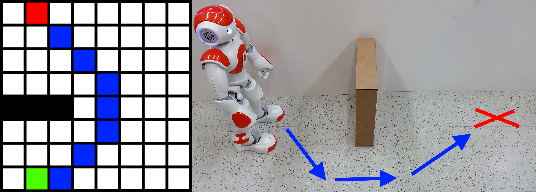
\includegraphics{nao_with_obstacle_and_map1.png}
	\caption
	{Example illustration of the Nao humanoid robot in an environment with an obstacle. The red X represents a goal
		location with the blue arrows showing an possible path. On the left side is one possible representation
		of the environment as a 2D grid.}
	\label{fig:nao_with_map1}
\end{figure}

\section{Background}
% Review previous work here as well.
% What is the problem of navigating, briefly.
% What is the problem of crawling, briefly.
% Why humanoids?
% Who's done humanoids before?
% Who's done navigation?
% We've done navigation.
% Who's done crawling?
% - Approaches to solving the problem - CPG actor critic paper
% We've done crawling.

\section{Platform Overview}
% As a medium we worked with the Nao. The Nao is good because this: stuff, stuff, stuff.
% The broader task of moving an agent from one location to another is applicable to a wide range of robots but
% each platform will have details that change the scope of the problem and the method used to approach it.
% The three problems focused on (local navigation, obstacle detection, and gaiting) for a flying robot with 
% a global camera system will require different solutions than a wheeled robot with only rangefinders.
% For this thesis, the Nao H25 V4 Humanoid Platform by Aldebaran Robotics was chosen to act as the mobile base. 
% With the future goal of having robots interact in human environments, humanoid platforms have become an active
% area of research as they are physically compatible with such environments. 
% While Nao is a 1.9 ft tall humanoid weighing 9.5 lbs and therefore only an appropriate analog for a young human toddler,
% the humanoid format is of primary importance to algorithmic development\.
% with 25 degrees of freedom including two legs, two arms, and two grippers. 
% Figure~\ref{fig:nao_diagram1} shows a cursory illustration of the humanoid configuration.
% This lightweight but capable configuration enables research into mobile manipulation, humanoid gaiting, and terrain adaptation
% without the need for specialized support equipment such as belays or dedicated experimentation areas as the
% robot is safe for humans to interact with.

\begin{figure}
	\centering
	\includegraphics[width=0.4\textwidth]{nao_coronal_highlighted2.png}
	\caption
	{Coronal view of the Nao humanoid with a few pertinent features highlighted. }
	\label{fig:nao_diagram1}
\end{figure}

% The robot comes with a suite of sensors including two cameras, two ultrasonic rangefinders, 
% a 3-axis accelerometer and 2-axis gyro, foot contact sensors, and angular position encoders on every joint.
% Such a complement of sensors aids the robot in creating an estimate of a number of variables including 
% the robot state and environment characteristics. 
% Nao has a built-in WiFi radio and 1.6 GHz Intel Atom processor running a version of the Linux operating system 
% allowing the robot to be programmed in C++ or Python using standard libraries that can be remotely uploaded.
% These features allow the use of a wide variety of tools when constructing new algorithms and for program
% iteration to happen at a rapid pace.
% 
% With all of these features the Nao makes for a convenient platform for the development of mobile robot algorithms.

% Then we stuck a Hokuyo laser on the Nao and used that for navigation. Why was this a good idea?
% To augment the sensor suite, a Hokuyo URG-04LX-UG01 Scanning Laser Rangefinder (Lidar) was mounted to the Nao and
% interfaced via a USB connection to the Nao's onboard computer. The sensor has a scanning area of $240^\circ$ with 
% an angular resolution of $0.36^\circ$ and a range of 5 meters. It is used to generate a planar point cloud representing
% the range to the nearest occlusion at a set of fixed bearing relative to the robot. Lidars are commonly used in mobile
% robotics so developing algorithms utilizing them is of practical concern.

% What equipment did we use?
% - Nao
% - Lidar
% - Mount
% Why did we use these things?

\section{Navigation}
% Briefly, what's navigation?
% What approach did we go for?
% Why did we go for this?

\section{Crawl Gait}

% Many robots that enjoy practical use are not mobile. They are affixed to a table or floor
% and do not depend on their environment in order to produce a commanded movement. They 
% utilize a motion model that describes how their parts interact with each other to move an
% end effector and typically avoid interacting with objects in their environment other than those
% they are required to manipulate.
% Mobile robots also use a motion model to plan their movements but, in contrast to fixed robots, must interact
% with their environment to produce movement. 
% While this can be a more challenging problem than motion planning for fixed robots, the use of
% the environment to produce motion leads to mobile robots having a richer and more adaptable set of movements.
% Aerial and aquatic vehicles push against water or air,
% wheeled robots roll over the ground, legged robots walk, run, and crawl.
% Not only can mobile robots operate through a wider set of environments than fixed robots, but different
% actuation schemes can be employed to produce different movements. Legged robots are a particularly interesting
% platform for ground locomotion, as opposed to wheeled platforms, because they are more adaptable
% to a wide range of environments by actuating their legs according to a different strategy.
% Collectively, the method by which legged robots actuate their legs as a function of time is called 
% gaiting. Different gaits produce different characteristics such as the range of
% achievable speeds, endurance, terrain adaptability and a host of other things.

% Briefly, what's crawling?
% Why crawling?
% What approach did we go for?
% Why did we go for this approach?

\section{Thesis Structure}
This thesis is organized as follows: 

% Chapter \ref{ch:platform} reviews the Nao Humanoid Platform with Hokoyu Scanning Laser Rangefinder augmentation.
% The navigation system is broken into three parts, 
% Chapter \ref{ch:navigation} discusses the GODZILA algorithm used for local navigation.
% Chapter \ref{ch:crawl_gait} discusses the Projected Profile crawling gait used to perform the crawl.
% Simulations and experimental results are shown in Chapters \ref{ch:simulations} and \ref{ch:results}, 
% while a discussion of the work is given in Chapter \ref{ch:conclusion}.

	%%%%%%%%%%%%%%%%%%%%%%%%%%%%%%%%%%%%%%%%%%%%%%%%%%%%%%%%%%%%%%%%%%%%%%%%%%%%%%%%%%
%%% Platform Description
%%% Add sample data from cameras and lidar
%%% Section 1 : Hardware Overview
%%%		SubSection 1.1 : Pertinent Nao Statistics (and how things talk to each other)
%%% 	SubSection 1.2 : Pertinent Lidar Statistics
%%%		SubSection 1.3 : Design Requirements for Lidar Mount and Description
%%% Section 2 : Software Framework
%%%		SubSection 2.1 : NaoQi and qibuild Overview
%%% 	SubSection 2.2 : Custom Library Framework
%%%		SubSection 2.3 : User Operation
%%%
%%%%%%%%%%%%%%%%%%%%%%%%%%%%%%%%%%%%%%%%%%%%%%%%%%%%%%%%%%%%%%%%%%%%%%%%%%%%%%%%%%
\chapter{Platform}\label{ch:platform}

For this thesis we used the Nao as the mobile platform. Aldebaran makes him.
He's a cool little robot and he allows us to explore both things we wanted to 
look at which were navigation and gaiting. He's mobile, small, ``cost-effective''
and has a good API that we can use to do lower-level control of things when we want to, 
and abstract ourselves from it when we don't want to.
The small size means he's easy to work with.

There's definitely some more opening paragraph to be written here about the Nao.
Probably say something about why he's useful to investigate crawling.
No one's going to send Nao into a disaster zone or anything but he's not too
far off from robots that you would send in and we don't have to spend all the 
money or build a new lab to work with him. You can do lot's of simulations, 
but in the end you still have to test on a real robot.

While the Nao is cool and all, the sonar sensors just don't cut it for what we want to do.
Lucky, Nao comes with a USB port and uses x86 and linux so it's relatively
straightforward to add new things to him. Therefore, we added a better distance sensor.
Specifically we added the Hokuyo URG-04LX-UG01.
It's a good Lidar because it has a respectable range, good angular resolution,
``cost-effective'', and is kinda lightweight. Using this sensor we could do mapping 
if we wanted to which means this system is extensible to the broader challenges 
of the overall navigation problem such as SLAM\@. Using the Lidar we'll be able to 
get enough information to do the job we need to.

While it's easy to plug a USB cable into Nao's head, you still have to stick the Lidar somewhere.
Nao doesn't have mount points that make it easy to add new hardware.
Given that we have a nifty 3D printer (and I know Solidworks) we designed up a little suit of
armor for Nao with a big stick coming out of it that we could mount the Lidar to, above his head.
This works but the new dynamics destabilize Nao's default gait at certain speeds. 
This doesn't mess with the navigation algorithm, but to increase the speed this will have to be dealt with,
either by changing the rig or \ldots using the arms to counterbalance the new inertial forces as
part of the walking gait.

\section{Hardware Overview}
% Ok so, three pieces of hardware here, the Nao, the Lidar, and the mount.
% Technically, all you need is the Nao since it is a mobile base with distance sensors but the sonars
% don't do that great so we added the Lidar, and since there's no where to screw it down we designed a mount.

The hardware assembled for this platform can be divided into three major parts,
the Nao H25 Humanoid Platform, a Hokuyo URG-04LX-UG01 Lidar, and a custom 3D
printed assembly to mount the Lidar to the Nao.
The Nao acted as the mobile base and provided onboard sensing and computation. 
Its large number of degrees of freedom and humanoid configuration were amenable
to the exploration of crawling algorithms.
The Nao is also equipped with two color cameras for viewing the environment
and two sonars for measuring the range to objects.
In the navigation experiment, the forward facing camera was used to estimate
the pose to a goal object. Though the two sonars can be used for obstacle
avoidance, previous experimentation showed they
were insufficient for use with navigation in a number of scenarios as
specular refections would cause confusing readings and the low angular
resolution would prevent the robot from walking through traversable apertures.
To supplement the Nao's sensor suite, the URG Lidar was mounted to the robot
to provide accurate, high resolution range data for use with navigation.
As the Nao does not have any external mounting points, a custom mount was
designed and constructed to allow the URG to be mounted to the Nao.


% Subsections about each hardware piece.
\subsection{Goal Object}
Like many navigation algorithms, the one used in Chapter~\ref{ch:navigation}
requires the platform to have a goal location for which to traverse.
For these experiments, the goal location was provided to the robot by means
of a physical object that the robot could detect with its onboard camera.
The Nao API provides a simple ``red ball'' tracker that can be used to track
red objects via the onboard camera. It provides not only bearing information
but also range by assuming the red object has a width of $0.06 m$.

The goal was built as a $0.127 m$ wide red cube. 
This was affixed to the top of a wooden dowel, mounted to a heavy wooden base to 
allow it to be easily placed.
Figure~\ref{fig:red_cube1} shows a picture of the cube.
The dowel was approximately $0.6 m$ tall to allow the robot to see the cube
while minimizing the amount the head needs to pitch in order to keep 
the cube in view. Building the cube to be wider than the 
expected width allowed the target to be seen by the robot from longer distances. 
This longer range allowed for the construction of a larger arena as well as more 
robust tracking at shorter ranges.
The goal was built as a cube rather than a ball because during testing 
the tracking algorithm did not seem to be affected by the change in geometry 
and a cube was easier to construct. 

\begin{figure}
\centering
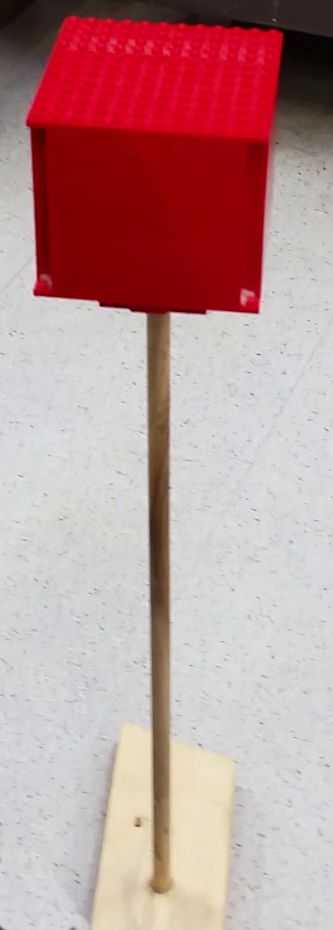
\includegraphics[height=0.4\textheight]{red_cube1.png}
\caption{Figure showing red cube the Nao tracked.}
\label{fig:red_cube1}
\end{figure}

\subsection{Nao Hardware}
The Nao Humanoid Platform is made by Aldebaran Robotics. 
Figure~\ref{fig:crrl_nao_coronal1} shows a picture of the Nao at the
Control/Robotics Research Lab of NYU Polytechnic School of Engineering.
The robot weighs $5.4 kg$ and has a maximum forward velocity over flat
terrain of approximately $1 \frac{m}{s}$.
It has 25 degrees-of-freedom (DoF) embodied via a 2 DoF head, two 5 DoF legs,
two 5 DoF arms, two 1 DoF hands, and a 1 DoF hip.
Figure~\ref{fig:nao_joints1} shows a diagram locating each of the joints on
the robot.
% Sonars, joint sensors, cameras, foot sensors, IMU, bumpers and buttons.
Each joint has an absolute angular position encoder, while the feet each have
four force sensitive resistors to detect ground contact.
The head has two color cameras, one that faces forward and the other that faces
downward to get a view of the terrain. The chest contains a 2-axis gyroscope and
a 3-axis accelerometer for inertial measurement, and two sonar transmitter-receiver
pairs for measuring the range to obstacles.
Figure~\ref{fig:nao_features1} shows a diagram locating the various robot sensors,
including those not listed above.
% Battery life, weight, top speed (before and after Lidar), sonar ranges, camera angles and pixels,
The sonars have a minimum range of $0.25 m$ and a maximum range of $2.55 m$.
They have a resolution of $1 cm$ and detect any obstacle within a $60^\circ$
cone. The cameras have a $1.22 Mp$ resolution, $30 Hz$ frame rate,
a horizontal field-of-view of $60.9^\circ$, and a vertical field-of-view of
$47.6^\circ$.
% CPU type and speed, RAM, storage space, USB, Ethernet, WiFi.
The robot is equipped with a 1.6 GHz Intel\textsuperscript{\textregistered}
Atom\textsuperscript{TM} CPU, 1 GB of RAM, and 2 GB of Flash memory.
It also has Gigabit Ethernet, 802.11 b/g/n WiFi, and USB 2.0. 
Nao's operating system is called NAOqi OS which is a customized version of
Gentoo Linux. Being a Linux distribution, the robot can be easily accessed
using ssh, scp, and ftp. This allows familiar command line tools to be used
to script behavior and manage services.
The robot can be natively programmed using the provided C++ or Python API.

% Ok, now briefly review what's to come in the subsubsections.
The Nao is a very feature rich platform suitable for a variety of autonomous
applications. The following sections will review specific aspects of the robot
relevant to Chapters~\ref{ch:results_navigation} and~\ref{ch:results_crawling}.


\begin{figure}
\centering
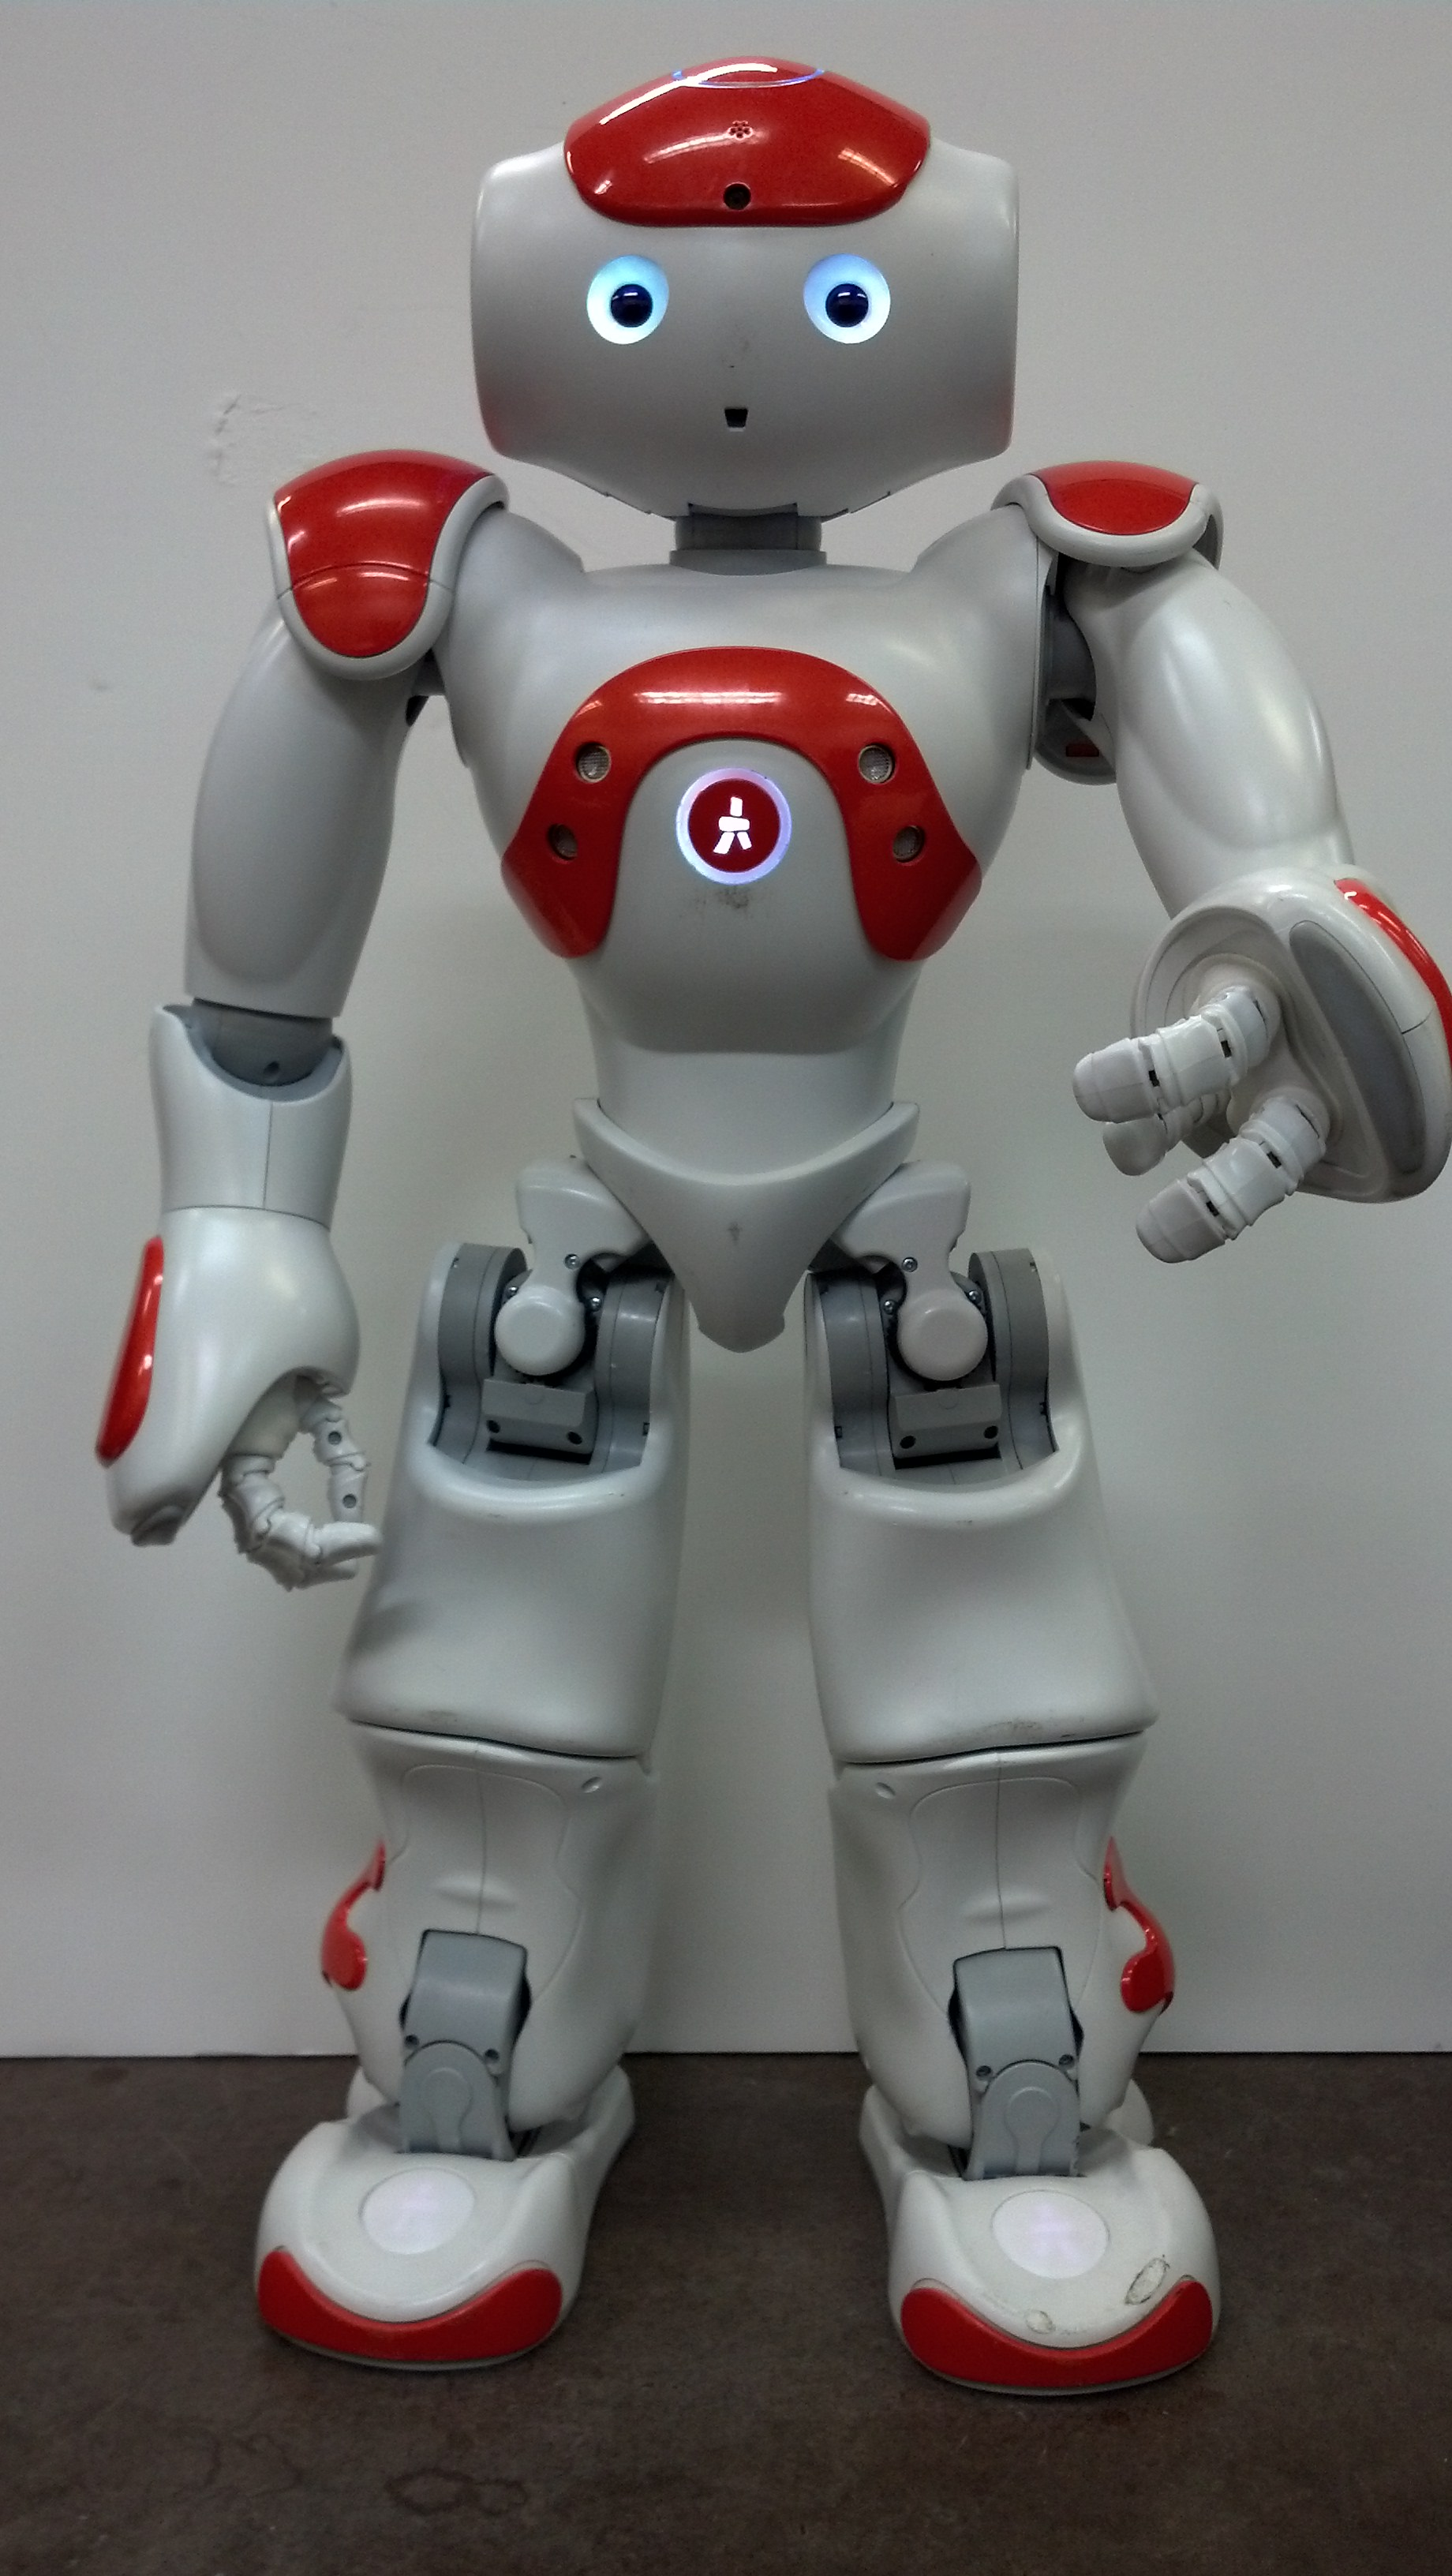
\includegraphics[height=0.4\textheight]{nao_coronal1.jpg}
\caption{Figure showing the Nao Humanoid Platform at the Control/Robotics
         Research Lab at NYU Polytechnic School of Engineering.}
\label{fig:crrl_nao_coronal1}
\end{figure}

\begin{figure}
\centering
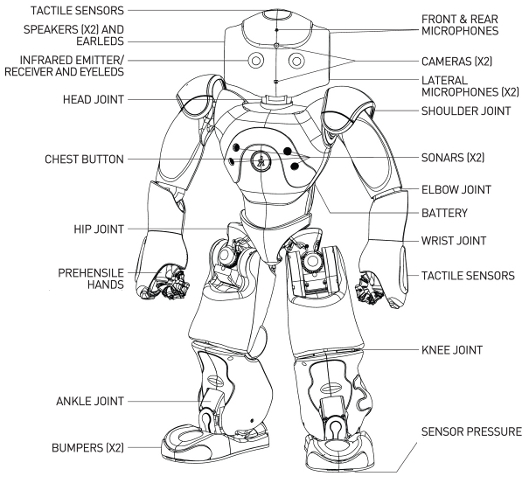
\includegraphics[width=0.4\textheight]{nao_diagrams/nao_h25_pres.png}
\caption{Figure locating the various features on the robot.}
\label{fig:nao_features1}
\end{figure}

\begin{figure}
\centering
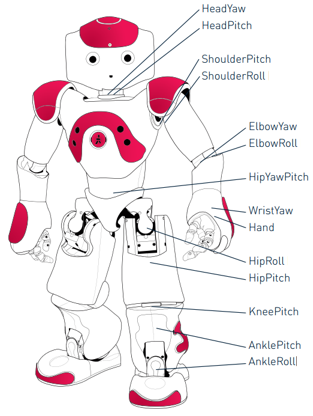
\includegraphics[height=0.4\textheight]{nao_diagrams/hardware_motortype_h25V5.png}
\caption{Figure indicating the various joint locations and their names.}
\label{fig:nao_joints1}
\end{figure}

\FloatBarrier

\subsubsection{Frame Definitions}
The NAOqi API defines three frames that can be seen in Figure~\ref{fig:nao_frames1}.
They are FRAME\_TORSO, FRAME\_ROBOT, and FRAME\_WORLD\@.
The first two frames, FRAME\_TORSO and FRAME\_ROBOT, are rigidly
attached to the robot, while FRAME\_WORLD is an inertial frame initialized
when the robot first starts.

\paragraph{FRAME\_TORSO} 
is a frame rigidly attached to the torso of the Nao. The positive Z-axis points
up through the head of the robot, while the positive X-axis points forwards.
It is useful for referencing different parts of the robot such and joint frames
and manipulation targets relative to the robot.
The frame origin along the X and Y directions is in the geometric center
of the torso, while Figure~\ref{fig:nao_link_lengths1} shows its Z location on
the torso as the point that the neck and hip offsets are referenced with
respect to.

\paragraph{FRAME\_ROBOT}
is a frame whose origin is between the feet of the robot. It's positive Z-axis
always points upwards and positive X-axis always points forwards. It is useful
when specifying navigation targets, relative to the Nao's current pose.

\paragraph{FRAME\_WORLD}
is a frame that is coincident with FRAME\_ROBOT when the Nao is started,
and remains static for the life of the run. It is useful for specifying navigation
and manipulation targets in a global coordinate sense.

\begin{figure}[H]
\centering
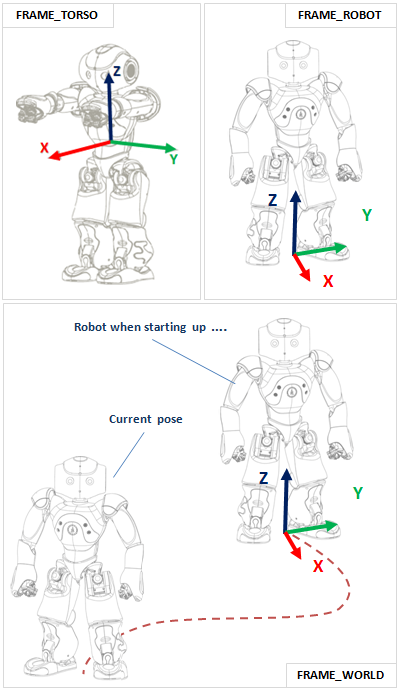
\includegraphics[height=0.75\textheight]{nao_diagrams/frame_definition_combo.png}
\caption{Nao frames.}
\label{fig:nao_frames1}
\end{figure}

Orientation targets for the Nao are commonly expressed using Tait-Bryan angles,
more commonly known as roll, pitch, and yaw. As can be seen in
Figure~\ref{fig:nao_rpy_def1}, yaw is expressed as rotation about the Z-axis,
roll is about the X-axis, and pitch is about the Y-axis.
When the robot is being referenced from the FRAME\_TORSO and is
initialized in the StandZero posture referenced in the proceeding section,
the naming conventions of the joints become clear. All joints whose axis
are parallel to the torso frame Y-axis are postfixed with the word ``Pitch'',
those parallel to the Z-axis are postfixed with the word ``Yaw'', and X-axis
with ``Roll''. The only exception to this rule is the ganged pelvis joint
axis. Each side of this degree of freedom rotates along a vector that is
in the plane formed by the torso Z-Y axes and is therefore postfixed with the
term ``YawPitch''.

\begin{figure}
\centerline{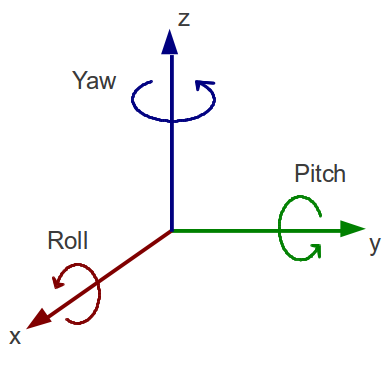
\includegraphics[width=0.5\textwidth]{nao_diagrams/rollPitchYaw.png}
}
\caption{Definition of roll pitch and yaw.}
\label{fig:nao_rpy_def1}
\end{figure}


\subsubsection{Links and Joints}
The Nao H25 is a bipedal platform with two legs, two arms, and an articulate
head. Each arm is composed of 5 joints and 3 non-zero length links, as are 
the legs, and the head is composed of 2 joints. There are also three fingers
per hand and two feet. Detailed measurements and specifications on the
Nao H25 can be found on the Aldebaran Website~\cite{nao_docs_h25}.
We will review a few relevant characteristics of the robot below.

\paragraph{Links}
Figure~\ref{fig:nao_link_lengths1} shows some of the large scale link lengths
of the Nao H25. The hip and neck Z offsets are measured with respect to
FRAME\_TORSO, as are the shoulder and hip Y offsets. The thigh and tibia lengths
are each roughly $100 mm$. Their total is $202.8 mm$. The neck and hip offsets
sum to $211.5$, making the torso approximately the same length as the legs.
The humerus of the robot is again nearly $100 mm$ though the forearm to the wrist
is half as long. The wrist to the hand is again about half as long as the
humerus, meaning in total, the arms are about as long and the legs.

\begin{figure}
\centerline{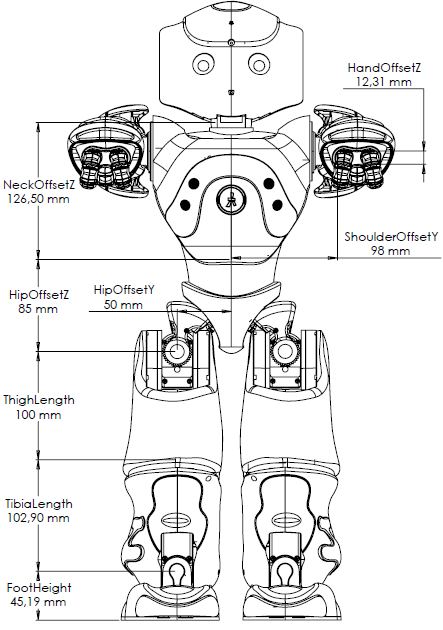
\includegraphics[width=0.45\textwidth]{nao_diagrams/hardware_lengthfront_3.3.png}
            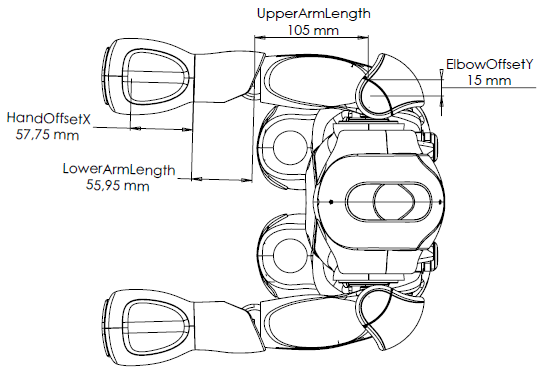
\includegraphics[width=0.55\textwidth]{nao_diagrams/hardware_lengthup_3.3.png}
}
\caption{Nao link lengths.}
\label{fig:nao_link_lengths1}
\end{figure}

\paragraph{Joints}
This needs to be said.
In the below diagrams, the green line represents the nominal zero, the blue line
is the min angle, and the red line is the max angle
\begin{figure}
\centering
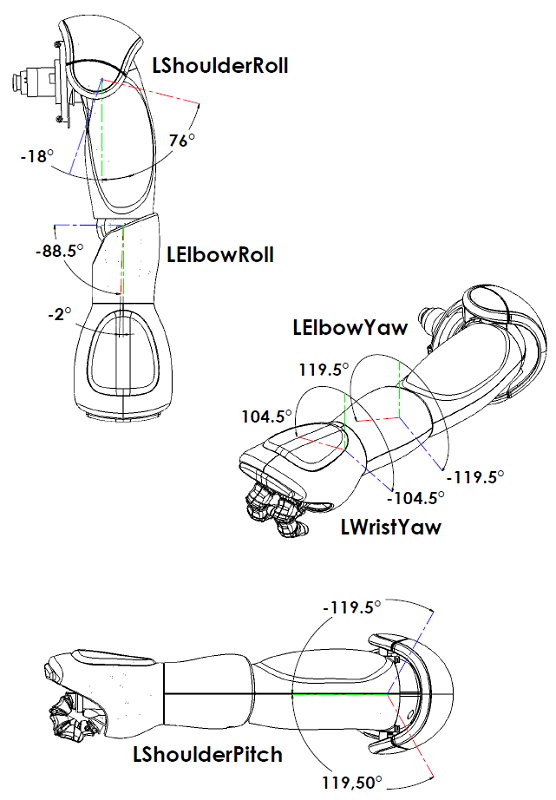
\includegraphics[width=\textwidth]{nao_diagrams/hardware_larmjoint_3.3_corr1.png}
\caption{Figure showing left arm}
\label{fig:nao_arm_joints_left1}
\end{figure}

\begin{figure}
\centering
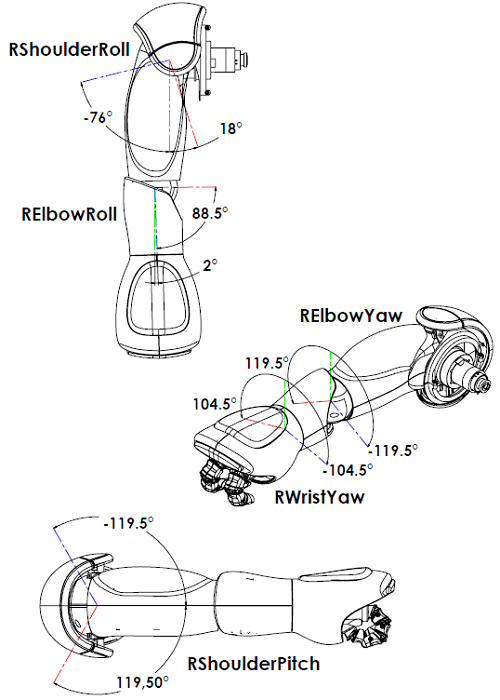
\includegraphics[width=\textwidth]{nao_diagrams/hardware_rarmjoint_3.3.png}
\caption{Figure showing right arm}
\label{fig:nao_arm_joints_right1}
\end{figure}

\begin{figure}
\centering
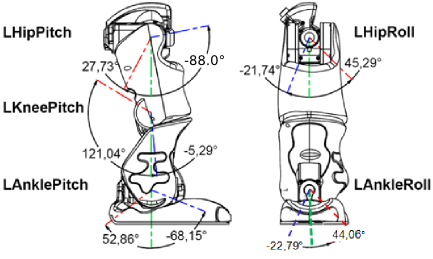
\includegraphics[width=\textwidth]{nao_diagrams/hardware_llegjoint.png}
\caption{Figure showing left leg}
\label{fig:nao_leg_joints_left1}
\end{figure}

\begin{figure}
\centering
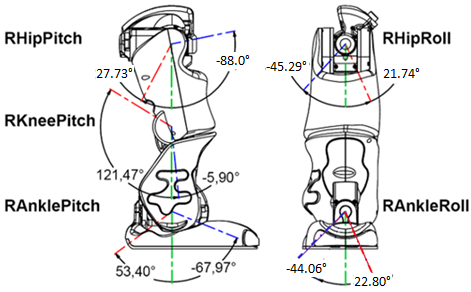
\includegraphics[width=\textwidth]{nao_diagrams/hardware_rlegjoint.png}
\caption{Figure showing right leg}
\label{fig:nao_leg_joints_right1}
\end{figure}

\begin{figure}
\centering
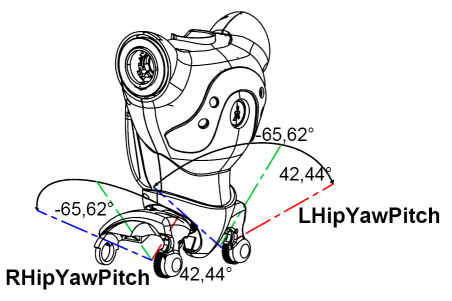
\includegraphics[width=\textwidth]{nao_diagrams/hardware_pelvisjoint.png}
\caption{Figure showing hip yaw-pitch}
\label{fig:nao_hip_yawpitch1}
\end{figure}

\paragraph{Arm Symmetry}
Need diagram showing arm symmetry for crawl results. 

\begin{figure}
\centering
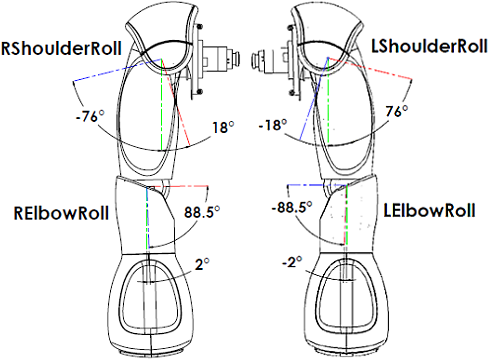
\includegraphics[width=\textwidth]{hardware_r_and_l_armjoint_corr1.png}
\caption{Figure showing arm joints and how they are a reflection.}
\label{fig:nao_arm_joints_reflect1}
\end{figure}

\FloatBarrier

\subsubsection{Joint Torques}
% Motor torques. (Important for Chapter~\ref{ch:crawl_gait})
Talking about the joint motor torques, tables, gearboxes, blah.

\subsubsection{Postures}
Talking about the different postures of the robot.

\begin{figure}
\centerline{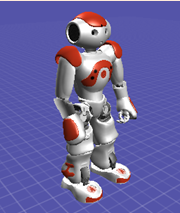
\includegraphics[width=0.33\textwidth]{posture/posture_stand.png}
            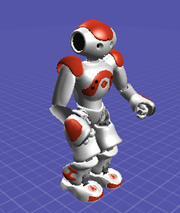
\includegraphics[width=0.33\textwidth]{posture/posture_standinit.png}
            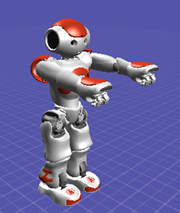
\includegraphics[width=0.33\textwidth]{posture/posture_standzero.png}
}
\vspace*{0.05in}
\centerline{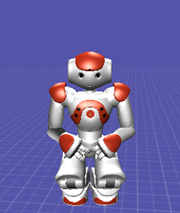
\includegraphics[width=0.33\textwidth]{posture/posture_crouch.png}
            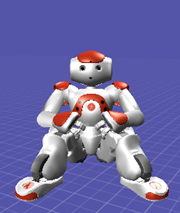
\includegraphics[width=0.33\textwidth]{posture/posture_sit.png}
            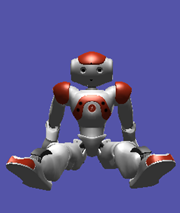
\includegraphics[width=0.33\textwidth]{posture/posture_sitrelax.png}
}
\vspace*{0.05in}
\centerline{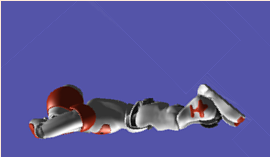
\includegraphics[width=0.5\textwidth]{posture/posture_lyingbelly.png}
            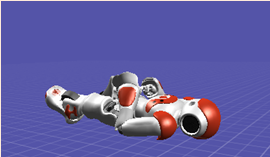
\includegraphics[width=0.5\textwidth]{posture/posture_lyingback.png}
}
\caption{Figure showing postures.}
\label{fig:nao_postures1}
\end{figure}

\subsection{Lidar Hardware}
The sensor used to detect environmental obstacles was a Hokuyo
URG-04LX-UG01, which can be seen in Figure~\ref{fig:lidar_top1}. 
The URG is a 2D scanning laser rangefinder, more commonly known as
a Lidar. Lidar is a portmanteau for \textit{Li}ght \textit{D}etection 
\textit{a}nd \textit{R}anging and operates using principles similar 
to Radar and Sonar. 2D Lidars provide a number of discrete range measurements
along a plane. This effectively gives a ``top-down'' or ``blue-print''
style view of an environment.
This, when mounted to a robot, allows the detection of objects in one plane of
the environment so that the robot can avoid or plan a path around them.

\begin{figure}
\centering
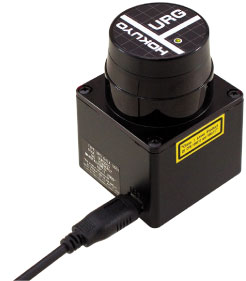
\includegraphics[height=0.3\textheight]{hokuyo/urg_04lx_ug01_top.jpg}
\caption{Photograph of the URG-04LX-UG01 Lidar. It is shown
         with a USB cable plugged in, which is the method of powering
         and retrieving data from the Lidar.}
\label{fig:lidar_top1}
\end{figure}

2D scanning Lidars such as the URG, sense the environment by emitting a laser
beam and measuring the time it takes for the emitted photons to return to the sensor.
This time is used to compute the range to the obstacle that the beam encountered.
Commonly, photons are not actually timed, but rather the phase difference of the
emitted light is used to estimate the time.
Following this measurement, the laser is then mechanically rotated to another 
angular position to take another reading. The process is repeated through the 
entire scanning angle of the sensor, and the set of range-angle pairs is 
considered ``one scan''. The URG uses a spinning mirror to rotate the beam, while
other sensors rotate the entire laser assembly.
An example of the data returned from the URG can be seen in Figure~\ref{fig:lidar_scan1}.
The URG was placed in a hall with a doorway to its left.

\begin{figure}
\centering
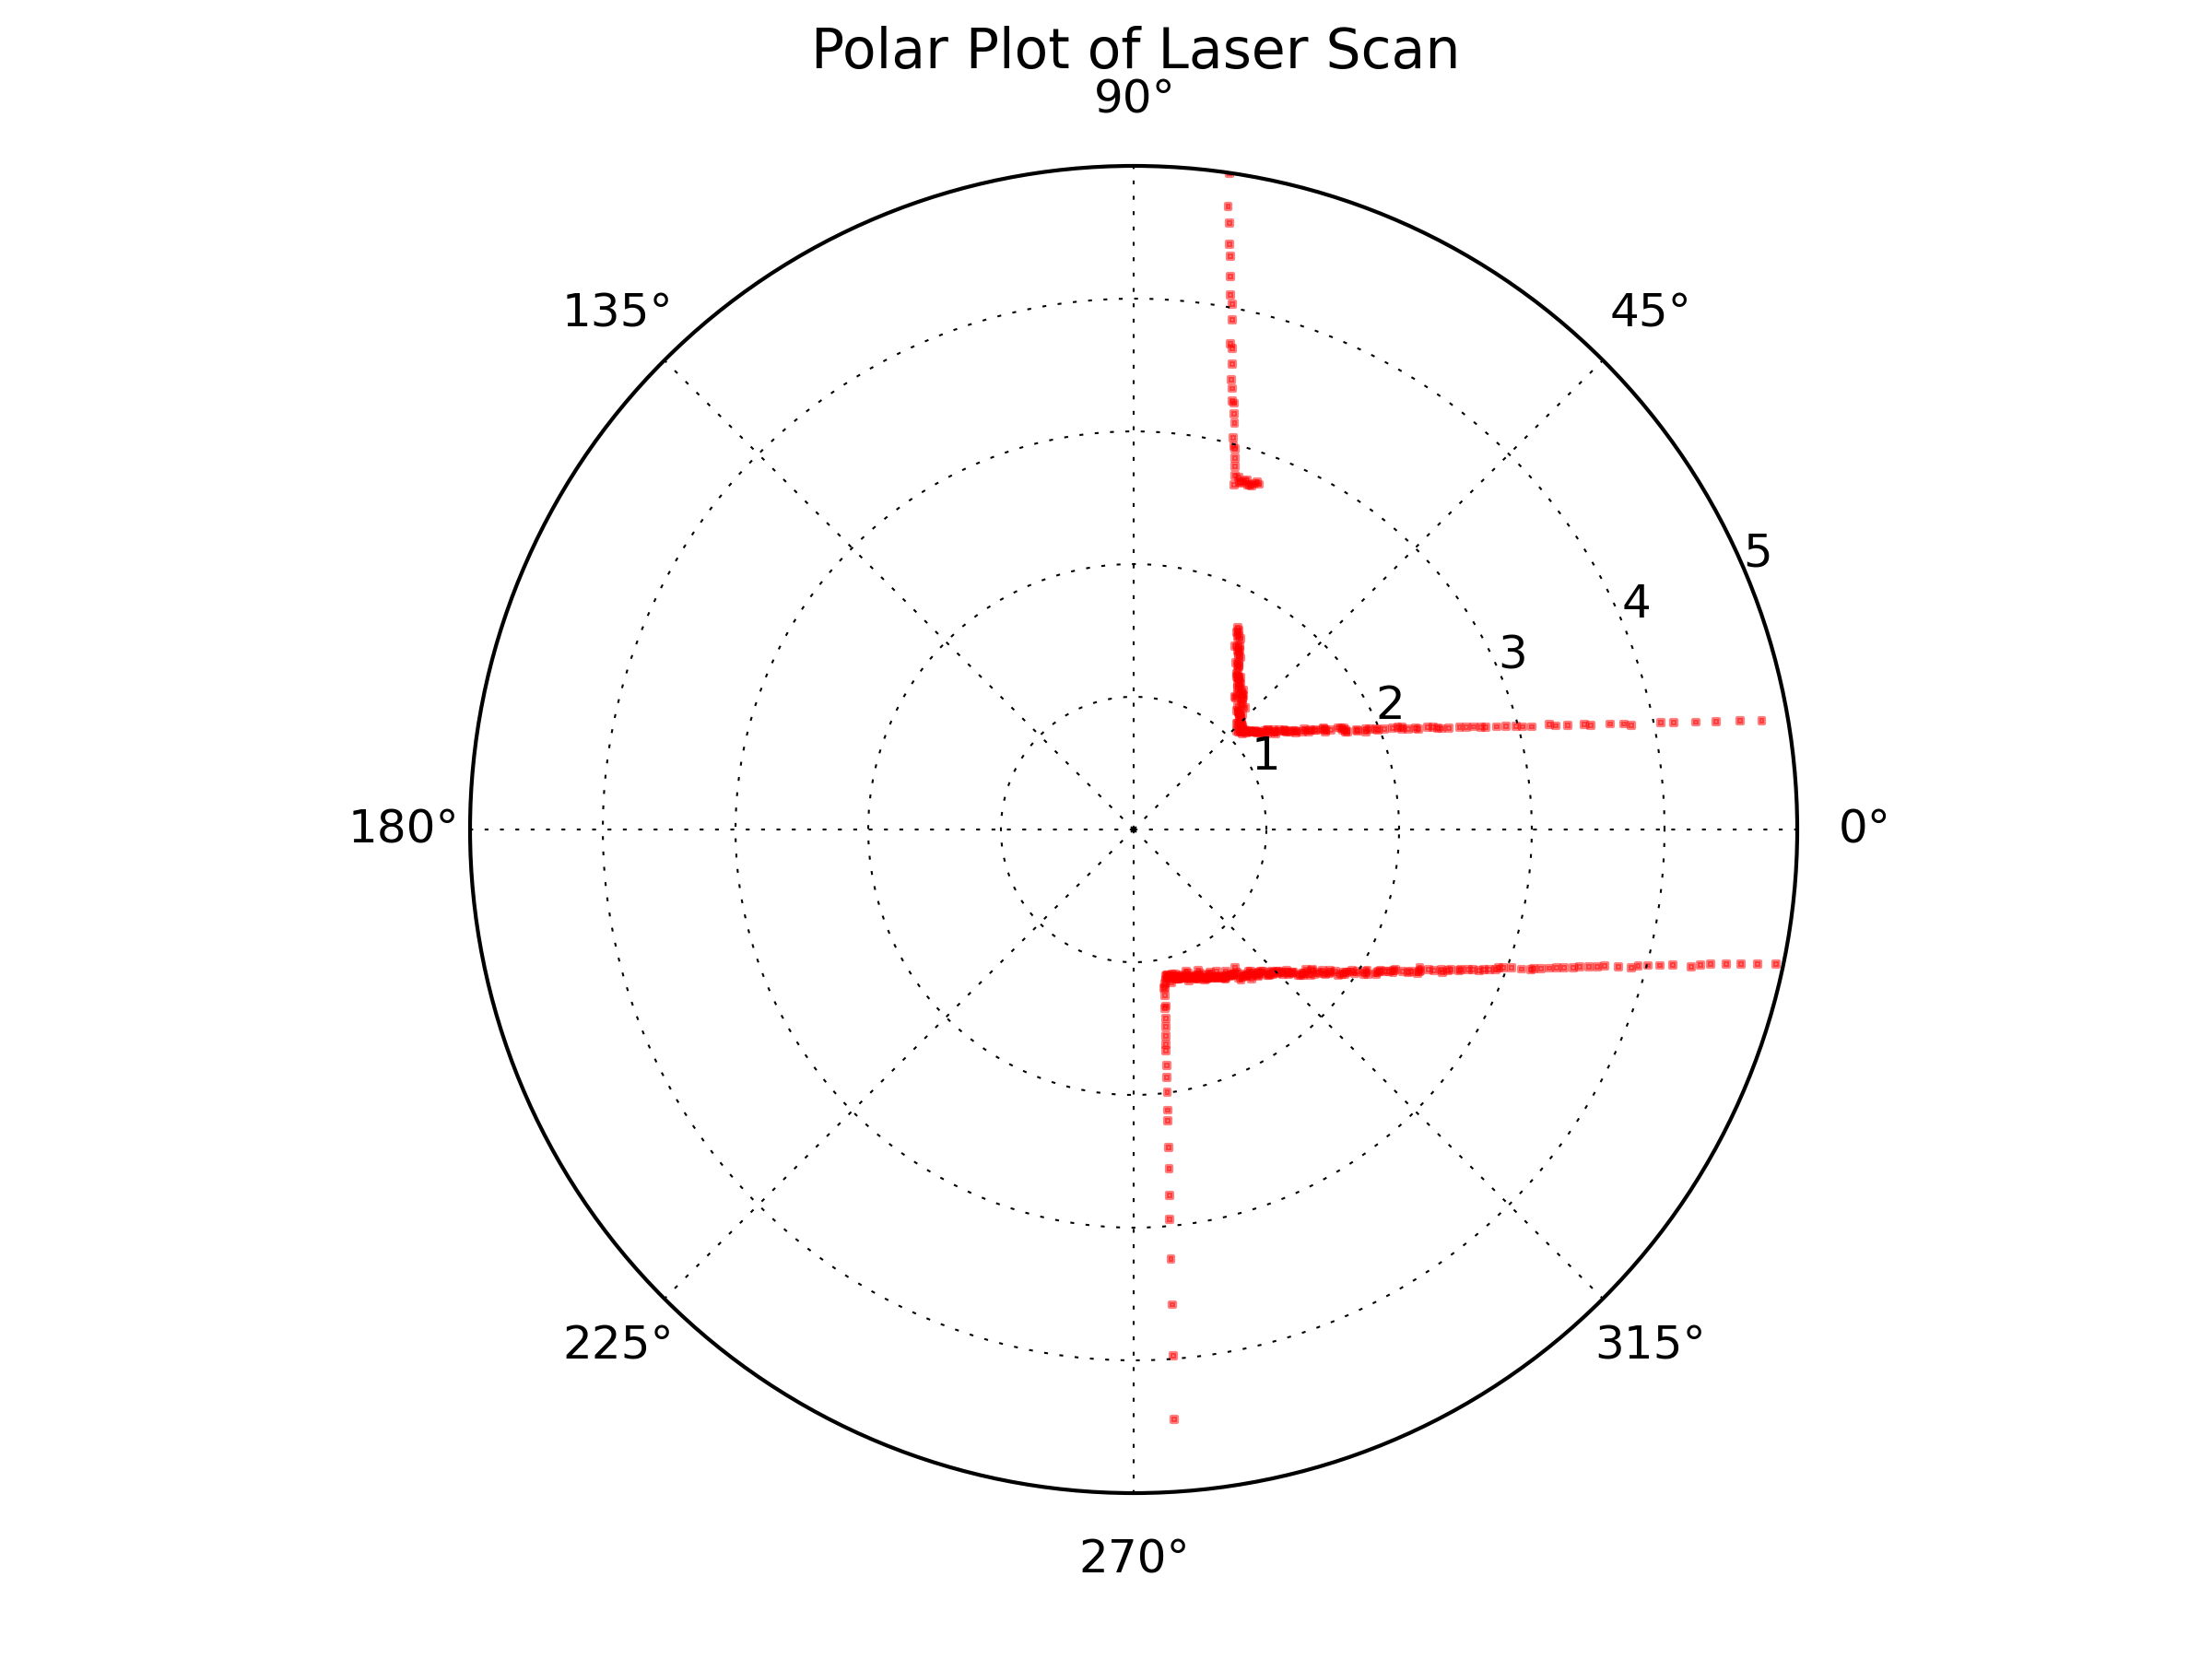
\includegraphics[height=0.4\textheight]{laser_scan_msg2.yaml_1.png}
\caption{Scan from the URG\@.
         The sensor is in the center of the figure.
         The radius of the figure is limited to 5 meters, which is 1 meter 
         greater than the maximum rated range of the sensor. While the unit will
         still provide data at this range, its accuracy is unrated.
         In this scan, the sensor is facing a hall, with a doorway to its left.}
\label{fig:lidar_scan1}
\end{figure}

The URG is a good choice for these experiments due to its lightweight and small
dimensions. This allows it to be easily mounted to the Nao Humanoid while
respecting the payload capacity of the robot. It has a wide scan angle, high
angular resolution, and a good range for this application. A high angular
resolution allows the robot to detect narrow obstacles that might obstruct the
robot's path, yet unlike sonar, provide detailed information about unobstructed
areas the robot can traverse. While the URG is rated for indoor use only, this
is sufficient for our application as the Nao is not often used in outdoor 
situations. Lastly, the sensor can be operated through a single USB port,
sourcing power from and providing data to the robot. This means no additional hardware is 
necessary for the Nao to make use of the sensor, as a USB port is available
in the back of the robot's head.
Figure~\ref{fig:lidar_diagram1} shows a mechanical drawing of the sensor, while
Table~\ref{tab:lidar_params1} lists some of the relevant specifications of the
URG.

\begin{table}
\centering
\begin{tabulary}{\textwidth}{|l||l|r|r|r|l|}
\hline
\textbf{Properties}& \textbf{Condition}         & \textbf{Min} & \textbf{Typ} & \textbf{Max} & \textbf{Units} \\	\hline\hline
\textbf{Scanner}   &                            &              &              &              &                \\	\hline
View Angle 	       &                            &              & 240          &              & degrees        \\	\hline
Angular Resolution &                            &              & 0.36         &              & degrees        \\	\hline
Range 	           &                            & 20           &              & 4000         & mm             \\	\hline 
Linear Resolution  &                            &              & 1            &              & mm             \\	\hline 
Accuracy           & Distance: 20 mm to 1000 mm &              & $\pm$ 30     &              & mm             \\	\hline 
        	       & Distance: 20 mm to 4000 mm &              & $\pm$ 3      &              & \%             \\	\hline \hline 
\textbf{Mechanical}&                            &              &              &              &                \\	\hline
Update Rate	       &                            &              & 100          &              & ms/scan        \\	\hline 
Weight             &                            &              & 160          &              & g              \\	\hline 
Width              &                            &              & 50           &              & mm             \\	\hline 
Length             &                            &              & 50           &              & mm             \\	\hline 
Height             &                            &              & 70           &              & mm             \\	\hline \hline
\textbf{Electrical}&                            &              &              &              &                \\	\hline 
Voltage Rating     &                            & 4.75         & 5.0          & 5.25         & V              \\	\hline 
Current Draw       &                            &              & 500          & 800          & mA             \\	\hline 
\end{tabulary} 
\caption{This table contains various specifications of the Hokuyo URG-04LX-UG01.
         These values were taken from the datasheet of the Lidar, which can be found here~\cite{urg_specs}.}
\label{tab:lidar_params1}
\end{table}

\begin{figure}
\centering
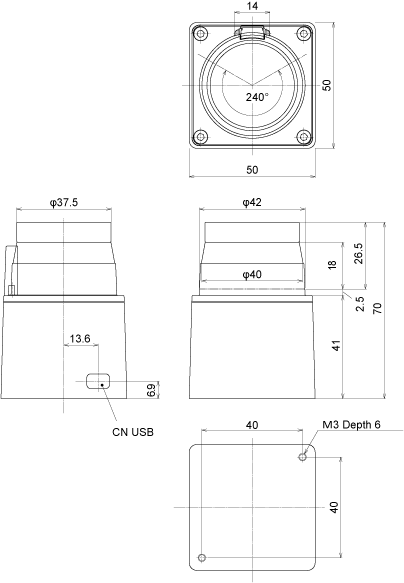
\includegraphics[height=0.3\textheight]{hokuyo/urg_04lx_ug01_ed.png}
\caption{Mechanical drawing of the URG-04LX-UG01.
         The compact size of the URG makes it easy to mount to the Nao.}
\label{fig:lidar_diagram1}
\end{figure}

\subsection{Lidar Mount}
% Design reqs: needed to rigidly attach to Nao for data transformation purposes, needed to see forward,
% lightweight, Nao needed to be able to move his head while wearing it,
% needed to be able to use the sonars (just in case).
In order to attach the URG Lidar to the Nao a custom Lidar mount was built.
The mount needed to hold the Lidar such that obstacles in front of the robot
could be sensed. The mount needed to be lightweight, rigidly attached, and allow
the robot to move its head to track the red cube. It should also not inhibit
the use of the sonars, in the event that the sonars are used in the future.

% Mounting it to the head seemed like it was going to be tough, so a vest was designed.
% Straps and foam seemed like they'd hold well enough. In fact they hold so well I can lift Nao up by the mount.
% The mount was made from PLA, 3D printer, foam, velcro straps.
As the Nao is not equipped with any mounting points, the Lidar mount was 
designed as a tray mounted to the front of the robot at waist-height, attached
using straps. The rigid parts were manufactured out of PLA plastic using a 3D
printer. The rigid parts that would contact the robot were padded with foam to
create a surface that would conform to the Nao's body and hold securely.
Figure~\ref{fig:nao_lidar_mount_nao_dimetric1} shows a CAD model of the finished
assembly.
A picture of the assembly mounted to the robot can be seen in
Figure~\ref{fig:nao_lidar_mount_picture1}.

\begin{figure}
\centering
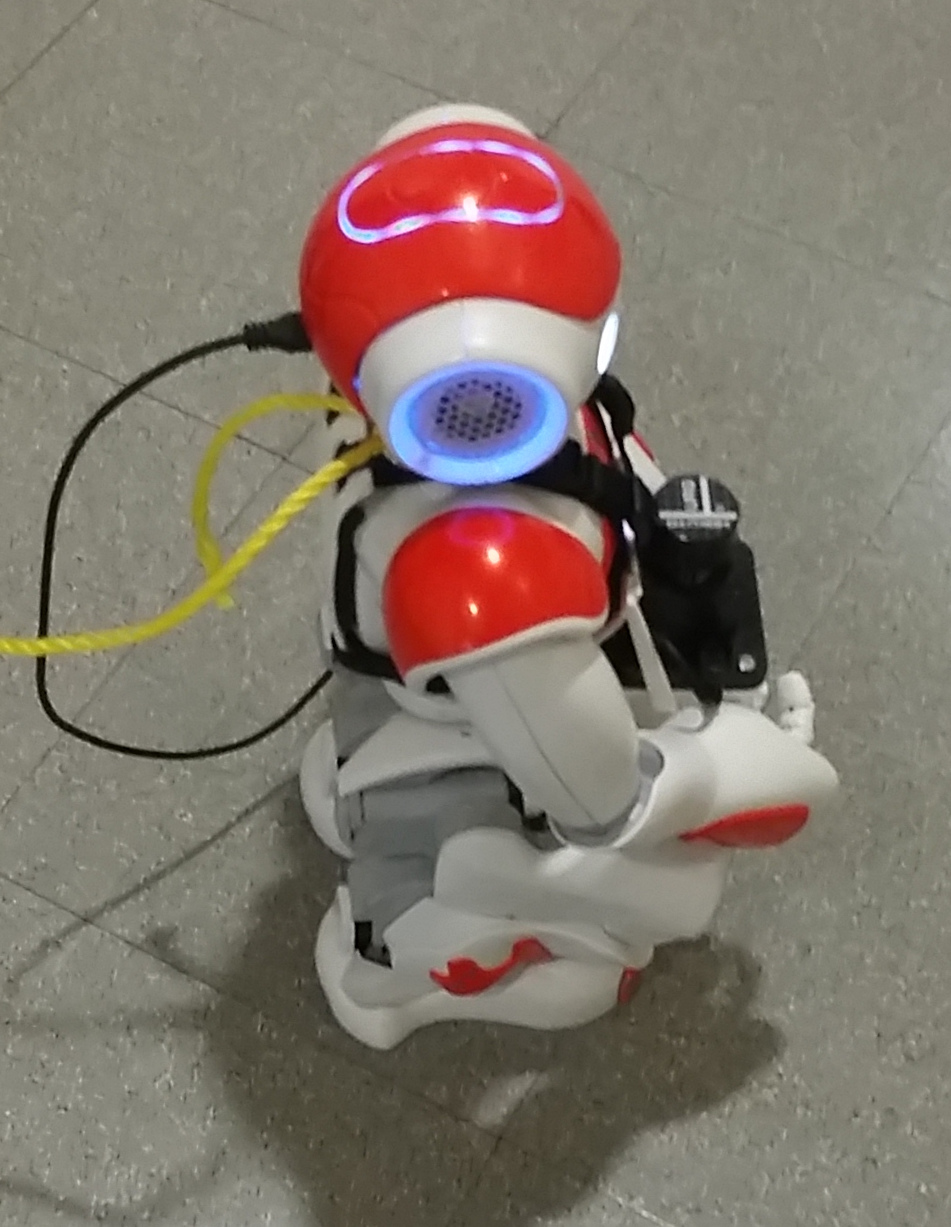
\includegraphics[height=0.4\textheight]{backpack/nao_with_mount2.jpg}
\caption{Figure showing a photograph of the URG mounted to the Nao using the
         custom Lidar mount.}
\label{fig:nao_lidar_mount_picture1}
\end{figure}

\begin{figure}
\centering
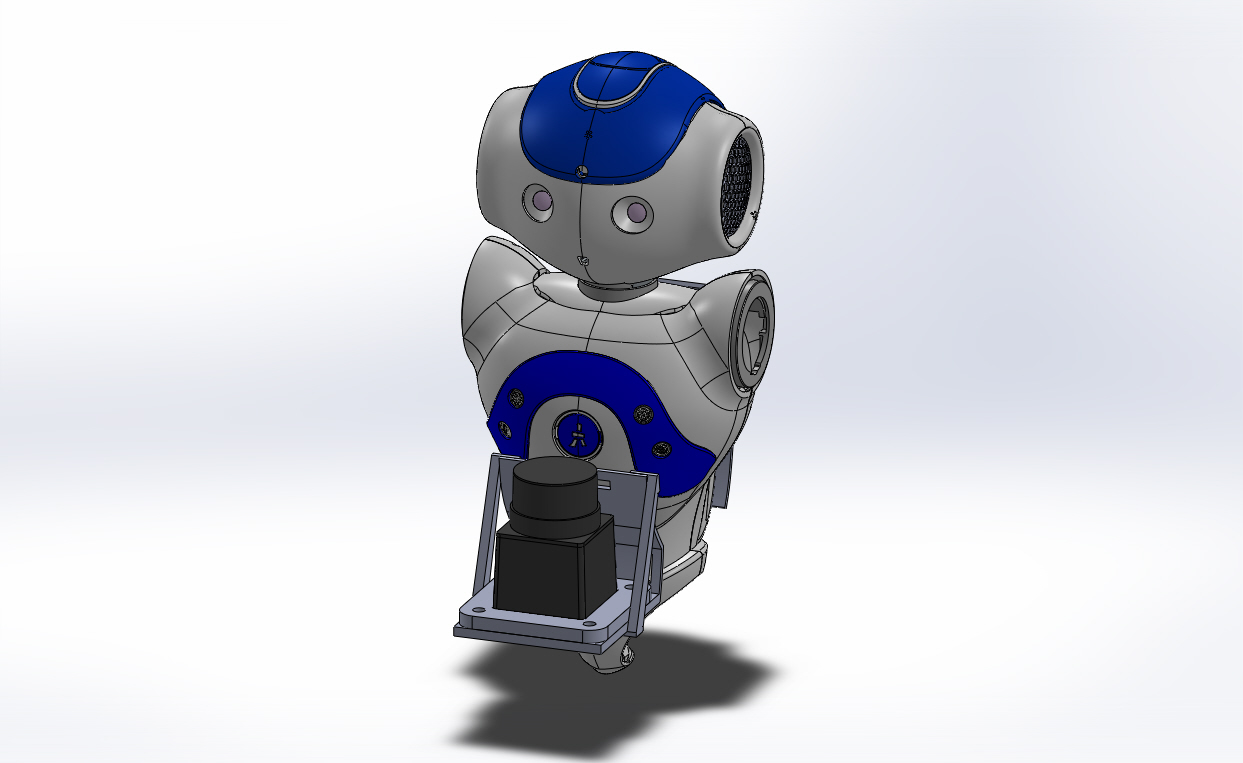
\includegraphics[height=0.4\textheight]{backpack/Assem_Nao_Dimetric1.jpg}
\caption{Figure showing CAD model of Nao with Hokuyo URG-04LX-UG01 mounted
         to the waist of the robot using a custom mount.}
\label{fig:nao_lidar_mount_nao_dimetric1}
\end{figure}

\begin{figure}
\centering
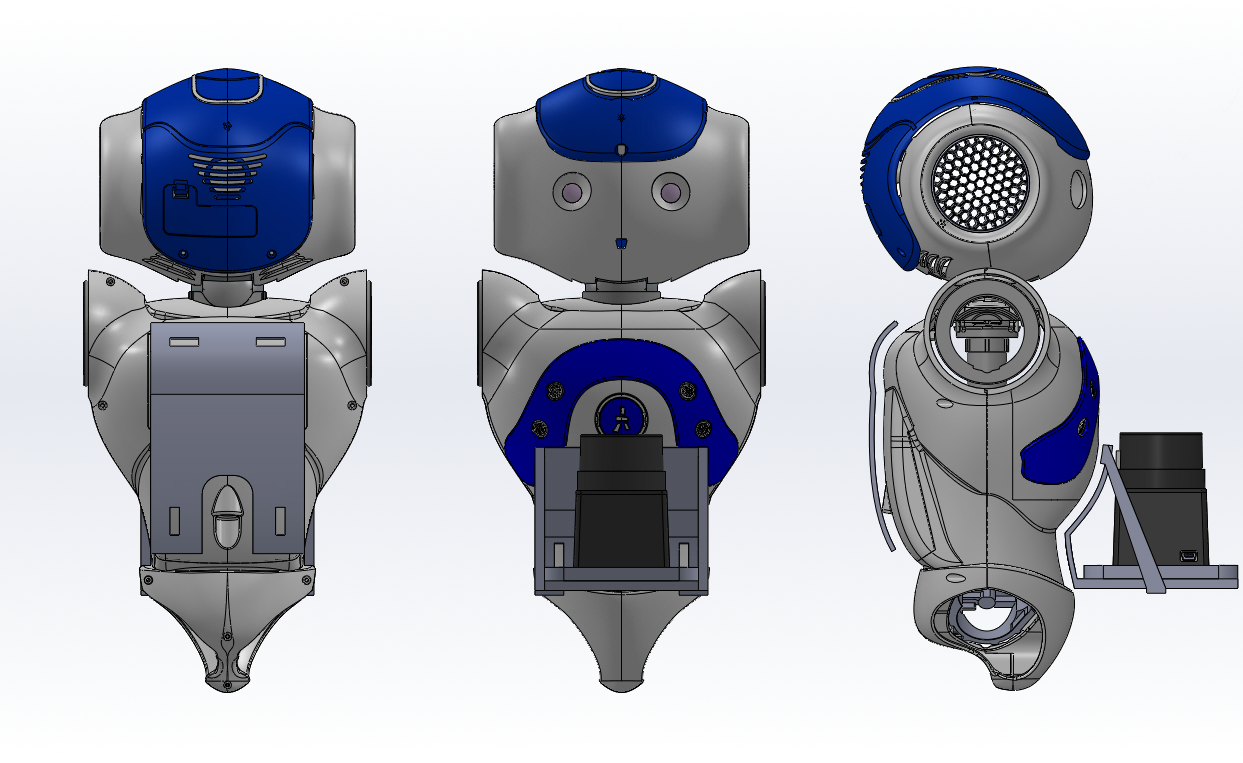
\includegraphics[height=0.4\textheight]{backpack/Assem_Nao_Three_View1.png}
\caption{Figure showing back, front, and side views of the URG CAD model 
         mounted to the Nao using the custom mount.}
\label{fig:nao_lidar_mount_nao_three_view1}
\end{figure}

The front subassembly of the Lidar mount consists of three parts: a front plate,
a base plate, and side supports. Figure~\ref{fig:nao_lidar_mount_dimetric1}
shows a CAD model of the assembled front subassembly with the URG installed.

\begin{figure}
\centering
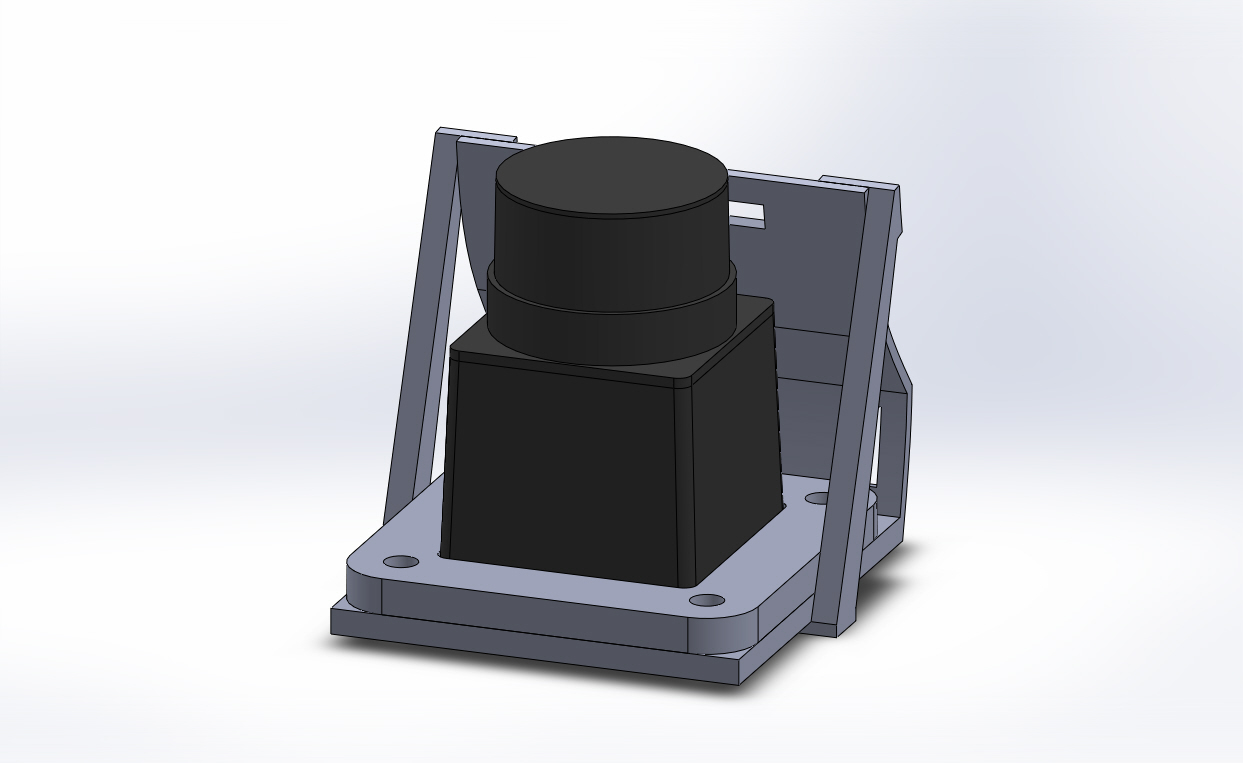
\includegraphics[height=0.4\textheight]{backpack/Assem_FrontOnly_Dimetric1.jpg}
\caption{Figure showing CAD model of the URG attached to the front subassembly
         of the custom Lidar mount.}
\label{fig:nao_lidar_mount_dimetric1}
\end{figure}

\begin{figure}
\centering
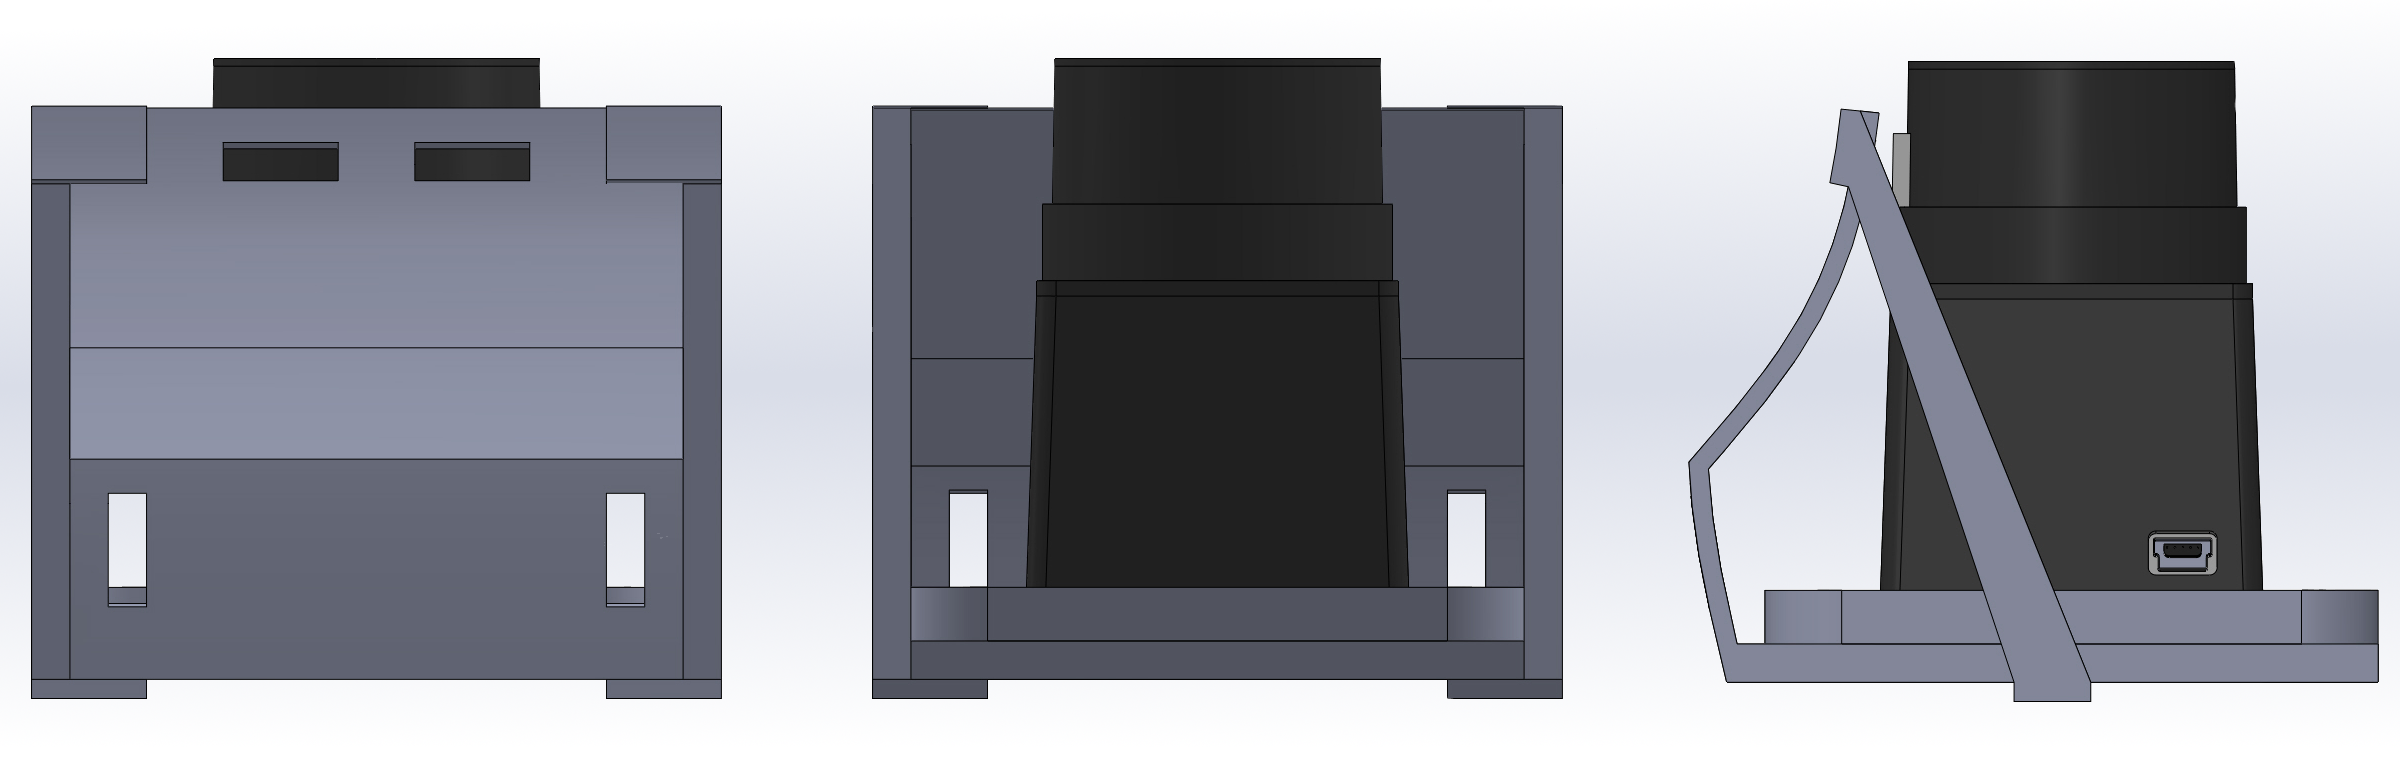
\includegraphics[width=\textwidth]{backpack/Assem_FrontOnly_Three_View1.png}
\caption{Figure showing back, front, and side views of the URG CAD model
         attached to the front subassembly of the custom mount.}
\label{fig:nao_lidar_mount_three_view1}
\end{figure}

The front plate has a shape that follows the form of the Nao.
It is padded with foam that is glued to the plate to conform to the robot more
closely and minimize the effects of vibration.
Figure~\ref{fig:nao_lidar_mount_frontplate_trimetric1} shows a CAD model of the
front plate. It has a tray that projects perpendicular from the robot to hold 
the base plate. Two mounting holes on the tray secure the base plate to the tray.
The front plate is secured to the robot via four rectangular holes which receive
velcro straps that go to the back plate. These straps are tightened to hold the
Lidar mount to the robot.

\begin{figure}
\centering
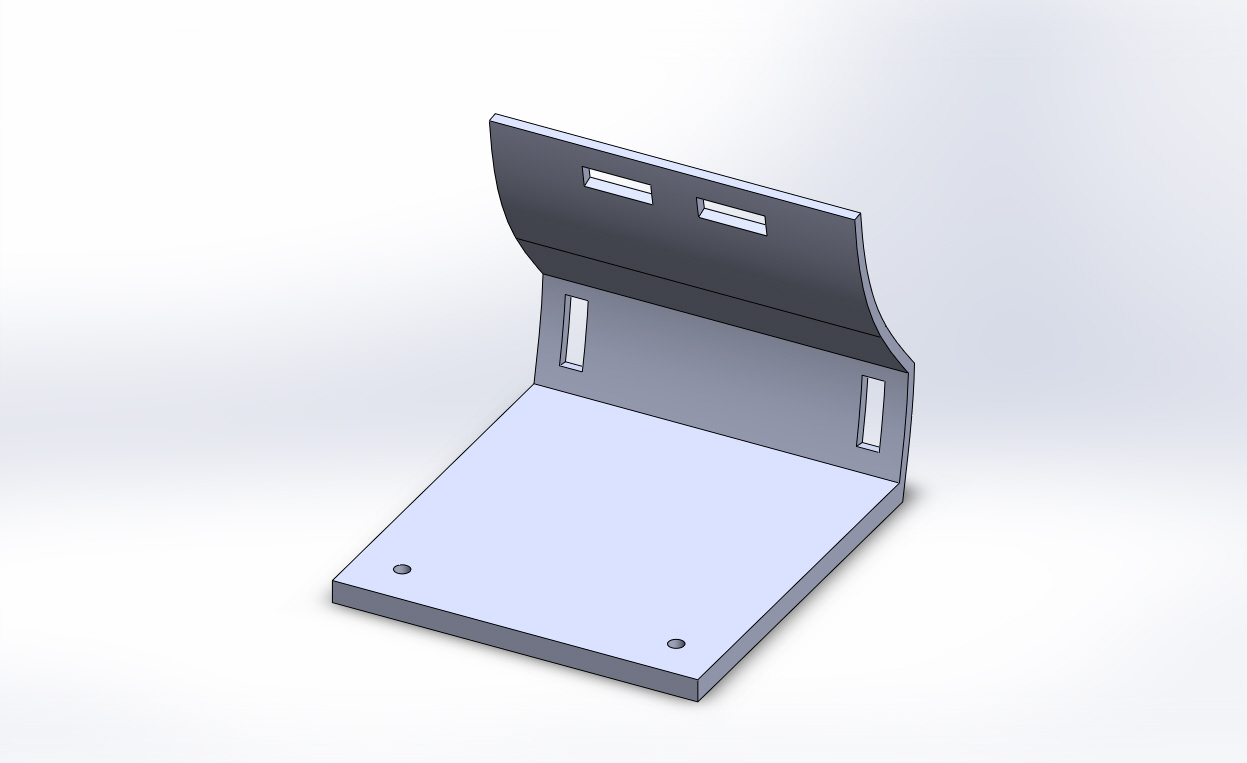
\includegraphics[height=0.4\textheight]{backpack/Front_Plate_Trimetric1.jpg}
\caption{Figure showing a CAD model of the front plate of the custom Lidar
         mount. The base plate attaches to this plate.}
\label{fig:nao_lidar_mount_frontplate_trimetric1}
\end{figure}

\begin{figure}
\centering
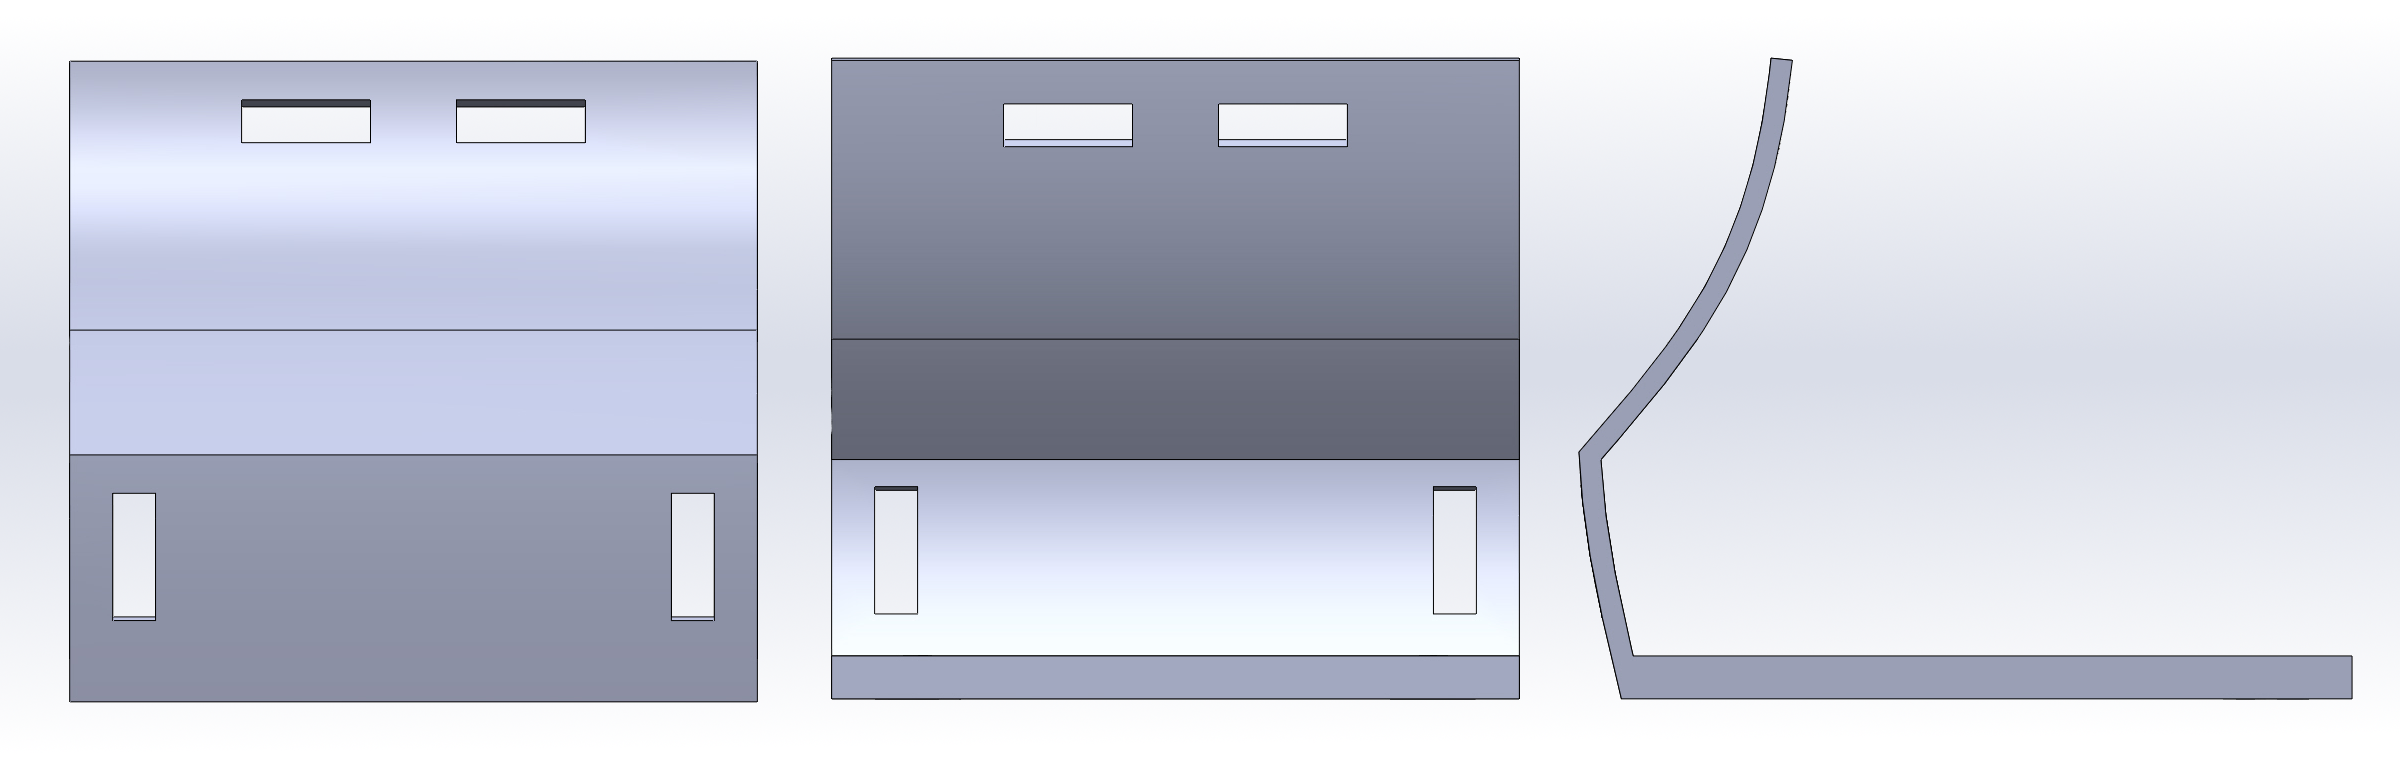
\includegraphics[width=\textwidth]{backpack/Front_Plate_Three_View1.png}
\caption{Figure showing back, front, and side views of the CAD model of the
         front plate.}
\label{fig:nao_lidar_mount_frontplate_three_view1}
\end{figure}

The URG is attached to the base plate, which in turn is attached to the 
tray of the front plate. The URG is attached to this intermediate part
rather than directly to the front plate to facilitate the mechanical
interoperability of different sensors to the front plate without needing
to produce different front plates for different sensors. Instead, different
base plates are made for different sensors. For example, the lower cost
RPLidar \cite{rp_lidar} or the VLP-16 Puck 3D Lidar
\cite{puck_lidar} are alternative Lidars that could
be mounted to the Nao for experimentation but have a different mounting 
configuration than the URG\@. In this way, new base plates can be manufactured
rather than front plates, allowing for a more modular design.

\begin{figure}
\centering
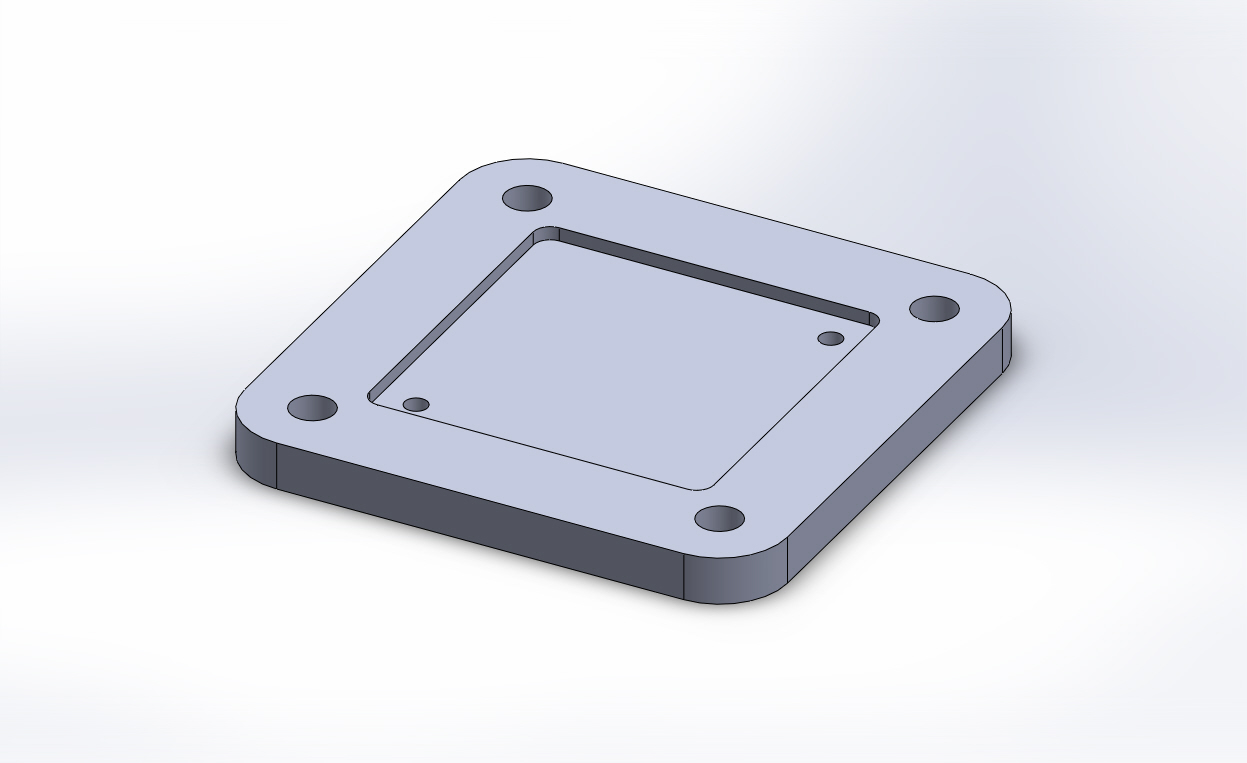
\includegraphics[height=0.4\textheight]{backpack/Base_Plate_Trimetric1.jpg}
\caption{Figure showing a CAD model of the base plate of the custom Lidar
         mount. The base plate is part of the front subassembly.
         The URG attaches to this plate.}
\label{fig:nao_lidar_mount_baseplate_trimetric1}
\end{figure}

\begin{figure}
\centering
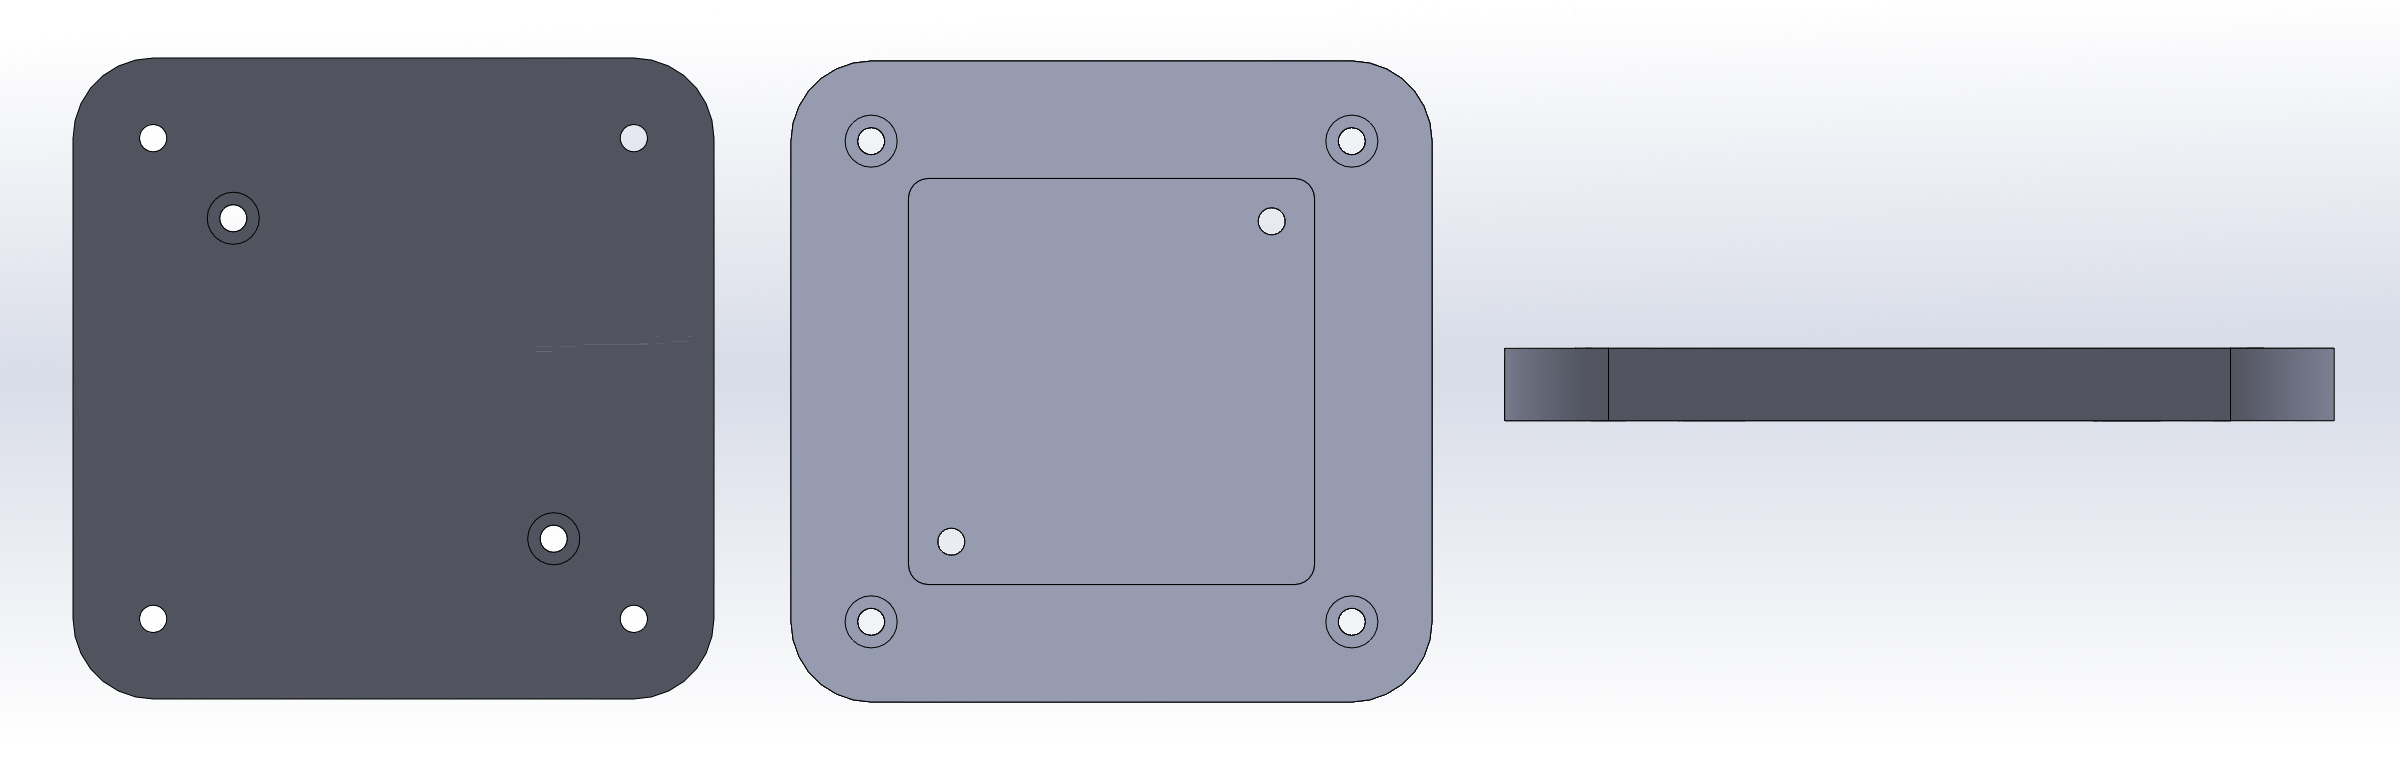
\includegraphics[width=\textwidth]{backpack/Base_Plate_Three_View1.png}
\caption{Figure showing back, front, and side views of the CAD model of the
         base plate.}
\label{fig:nao_lidar_mount_baseplate_three_view1}
\end{figure}

\begin{figure}
\centering
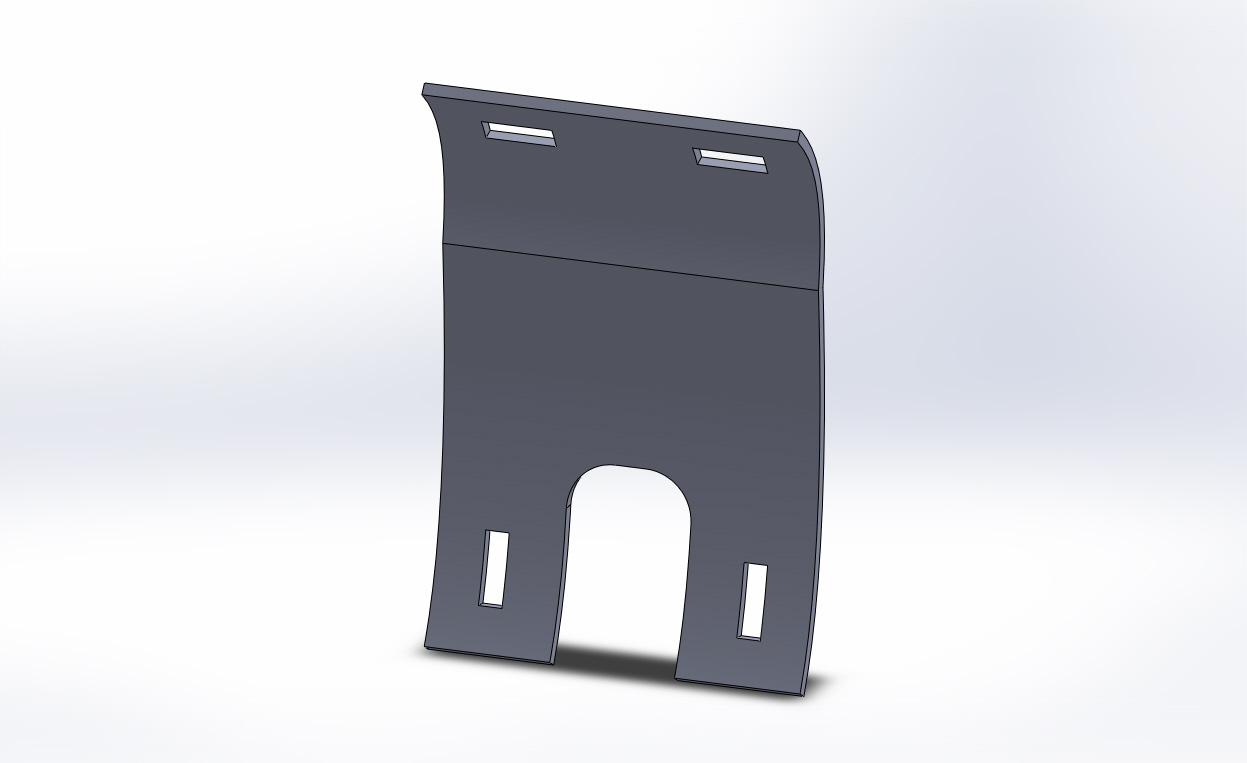
\includegraphics[height=0.4\textheight]{backpack/Back_Plate_Dimetric1.jpg}
\caption{Figure showing a CAD model of the back plate of the custom
         Lidar mount.}
\label{fig:nao_lidar_mount_backplate_dimetric1}
\end{figure}

\begin{figure}
\centering
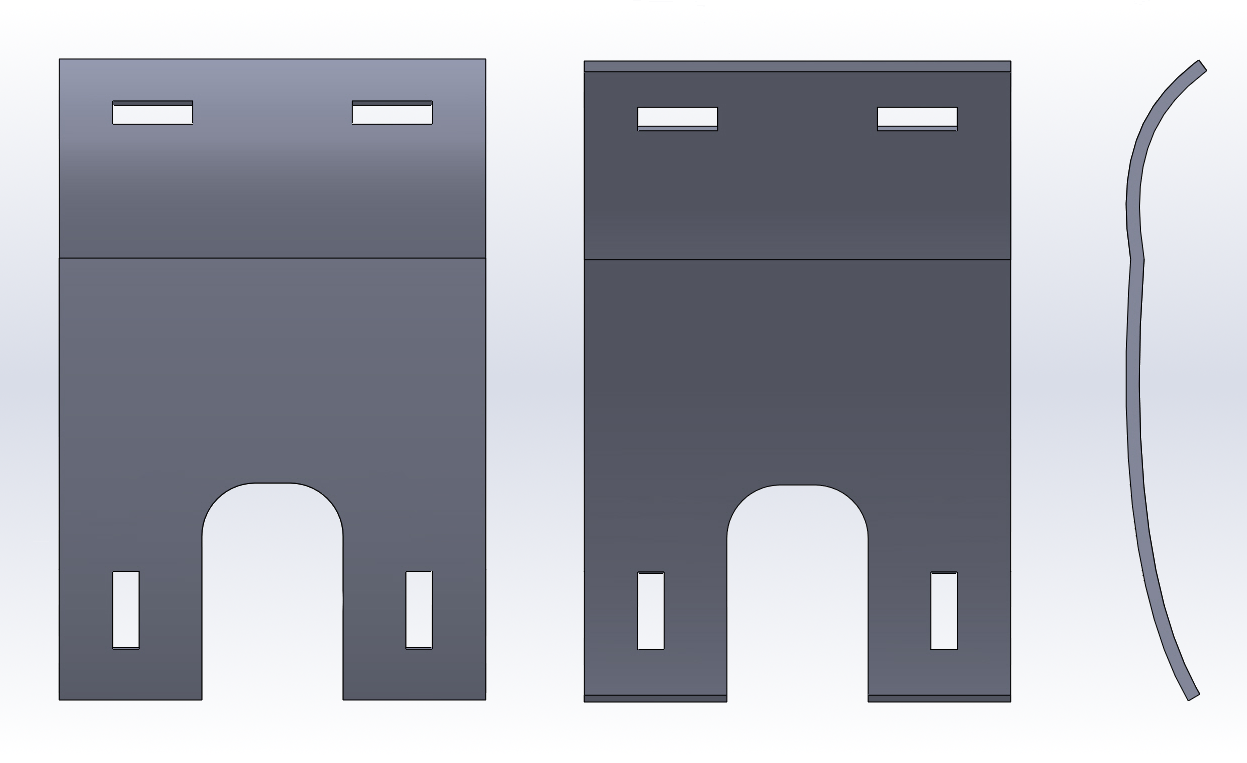
\includegraphics[width=\textwidth]{backpack/Back_Plate_Three_View1.png}
\caption{Figure showing back, front, and side views of the CAD model of the
         back plate of the custom Lidar mount.}
\label{fig:nao_lidar_mount_backplate_three_view1}
\end{figure}



\begin{figure}
\centering
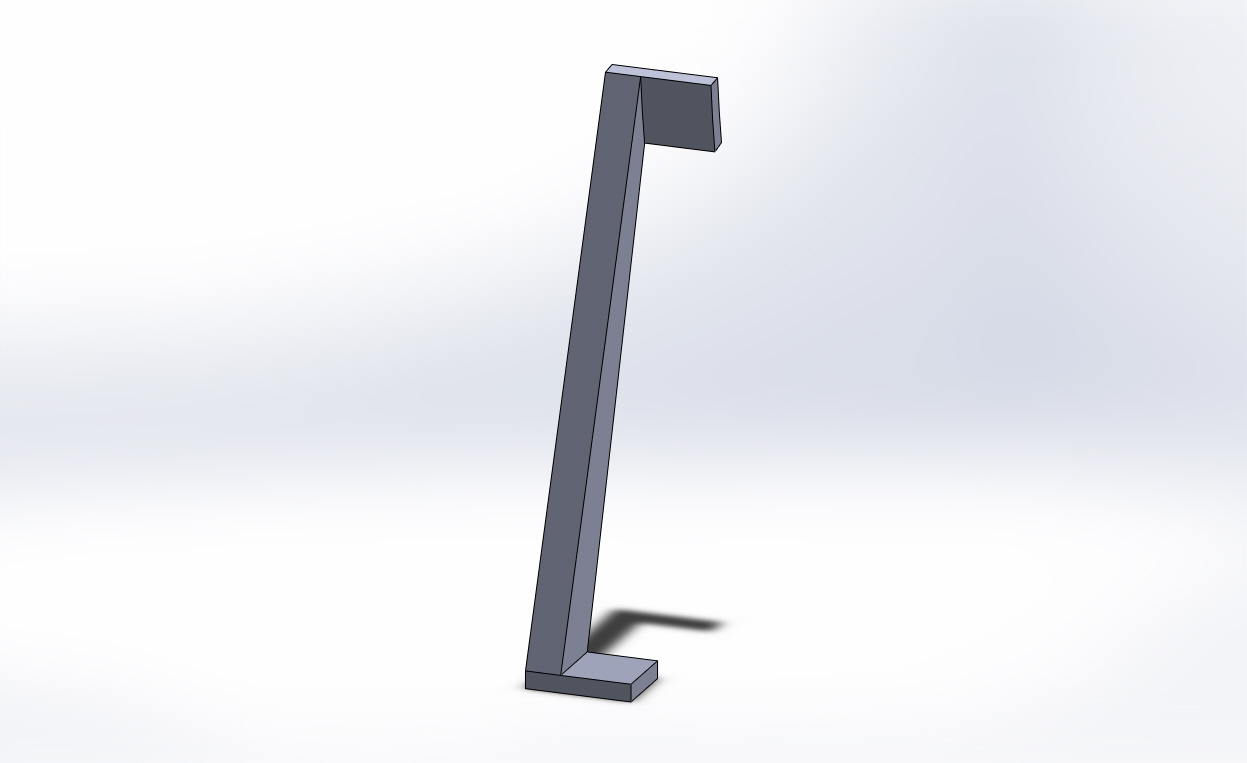
\includegraphics[height=0.4\textheight]{backpack/Support_Left_Trimetric1.jpg}
\caption{Figure showing a CAD model of the left side support of the custom
         Lidar mount. This support is bonded to the front plate to add rigidity
         to the front plate. The right side support is a mirror image of this
         part.}
\label{fig:nao_lidar_mount_supportleft_trimetric1}
\end{figure}

\begin{figure}
\centering

\includegraphics[height=0.4\textheight]{backpack/Support_Left_Three_View1.jpg}
\caption{Figure showing back, front and side views of the CAD model of the left
         side support.}
\label{fig:nao_lidar_mount_supportleft_three_view1}
\end{figure}


% Need some sort of System or summary Section.

	
%%%%%%%%%%%%%%%%%%%%%%%%%%%%%%%%%%%%%%%%%%%%%%%%%%%%%%%%%%%%%%%%%%%%%%%%%%%%%%%%%%
%%% Navigation
%%% 
%%% Section 1 : Survey of Algorithms
%%% 	Subsection 1.1 : Classes of Algorithms
%%% Section 2 : Potential Fields
%%%	Section 3 : GODZILA
%%% mention that one aspect of navigation is vertically constrained spaces, connect to next chapter
%%%%%%%%%%%%%%%%%%%%%%%%%%%%%%%%%%%%%%%%%%%%%%%%%%%%%%%%%%%%%%%%%%%%%%%%%%%%%%%%%%
\chapter{Navigation}\label{ch:navigation}

%%% What is navigation? %%%
% Make this section less colloquial.
Navigation is the task of generating a series of commands that allow a robot to transit from its current pose
to some goal pose. This task encompasses a number of subtasks such as path planning, environment sensing, and obstacle
avoidance. As a robot transits through space from its current to goal pose, it necessarily visits a series
of intermediate poses the choice of which depends on its kinematic constraints and the constraints of the environment it transits through. 
Collectively, this set of poses as a time sequence is known as a path. 
The spacial region in which the robot operates is known as the task space and all kinematically feasible configurations is known as the
configuration space.  Typically, the environment a robot traverses is not free space but also contains obstacles 
which constrain the paths which can be taken to the goal. While in some 
controlled environments the location of obstacles can be known \textit{a priori} and supplied to the robot in the form of a map, often the
robot will have the task of creating a map which describes the location of these obstacles. In some situations, ``global'' 
sensors can view the entire environment within which the robot will operate and can capture all of the constraints while in others (especially
in the case of mobile robots) only ``local'' sensors mounted to the robot are available to detect environmental limitations
to the robot's path as they are encountered. Even more challenging is the case where the environmental obstacles are not
static but are moving adding a time varying element to the obstacle avoidance problem.

% In the first place that you mention the categories, you can clarify that the categories are not mutually exclusive,
% but that algorithms are classified into combinations of categories.

% Algorithms that solve the navigation problem are sometimes described according to four major categories.

% Here's one way to split up things:
Algorithms that solve the navigation problem are sometimes described according to four major categories (though there are many
other categories with which these algorithms could be described with). These categories are not mutually exclusive, and algorithms
are commonly attributed with multiple classifications.
The first two, known as global or local, speak to the amount
of spatial data or time horizon considered when planning a solution. If only a short time horizon or occlusions in the immediate
spatial region are accounted for, then the algorithm is considered local, otherwise it is thought of as global.
The other two deal with how the spaces or paths are represented, continuously or discretely. If the algorithm breaks
up these spaces into finite resolution pieces, then it is discrete. Continuous algorithms choose some sort of parameterization
to the spatial or environmental constraints using a model. Often algorithms are some mixture of all of these four categories.

The algorithm used for navigation in this thesis is the GODZILA navigation algorithm, 
which can be categorized as a local continuous algorithm based on the potential fields navigation strategy. 
While in many environments GODZILA solves the navigation problem, it can also be used in conjunction with global algorithms
that can plan way points to the goal without having to consider the detailed local environment.

%%% Addendum's %%%
In the design on the obstacle avoidance algorithm for a robot, it is important to consider how different local sensors 
can affect the choice of navigation algorithm. The Nao humanoid platform
used in this thesis is equipped with two sonar sensors for obstacle detection. Details on these are given in Chapter~\ref{ch:platform}.
These sensors have a broad angular range and cannot provide information about where within this cone obstacles are located.
This enables the robot to avoid colliding with objects directly in front of it but might cause the obstacle avoidance algorithm
to preclude the discovery of possible paths (e.g., narrow corridors between obstacles).
Conversely, scanning laser rangefinders (such as the one mounted to the Nao and described in Chapter~\ref{ch:platform}) have a
very high degree of angular resolution and provide hundreds of range measurements. This allows for a more accurate description
of environmental occlusions allowing more paths to be considered for traversal.
% [Insert picture of sonar cones vs lasers.]
\begin{figure}
\centering
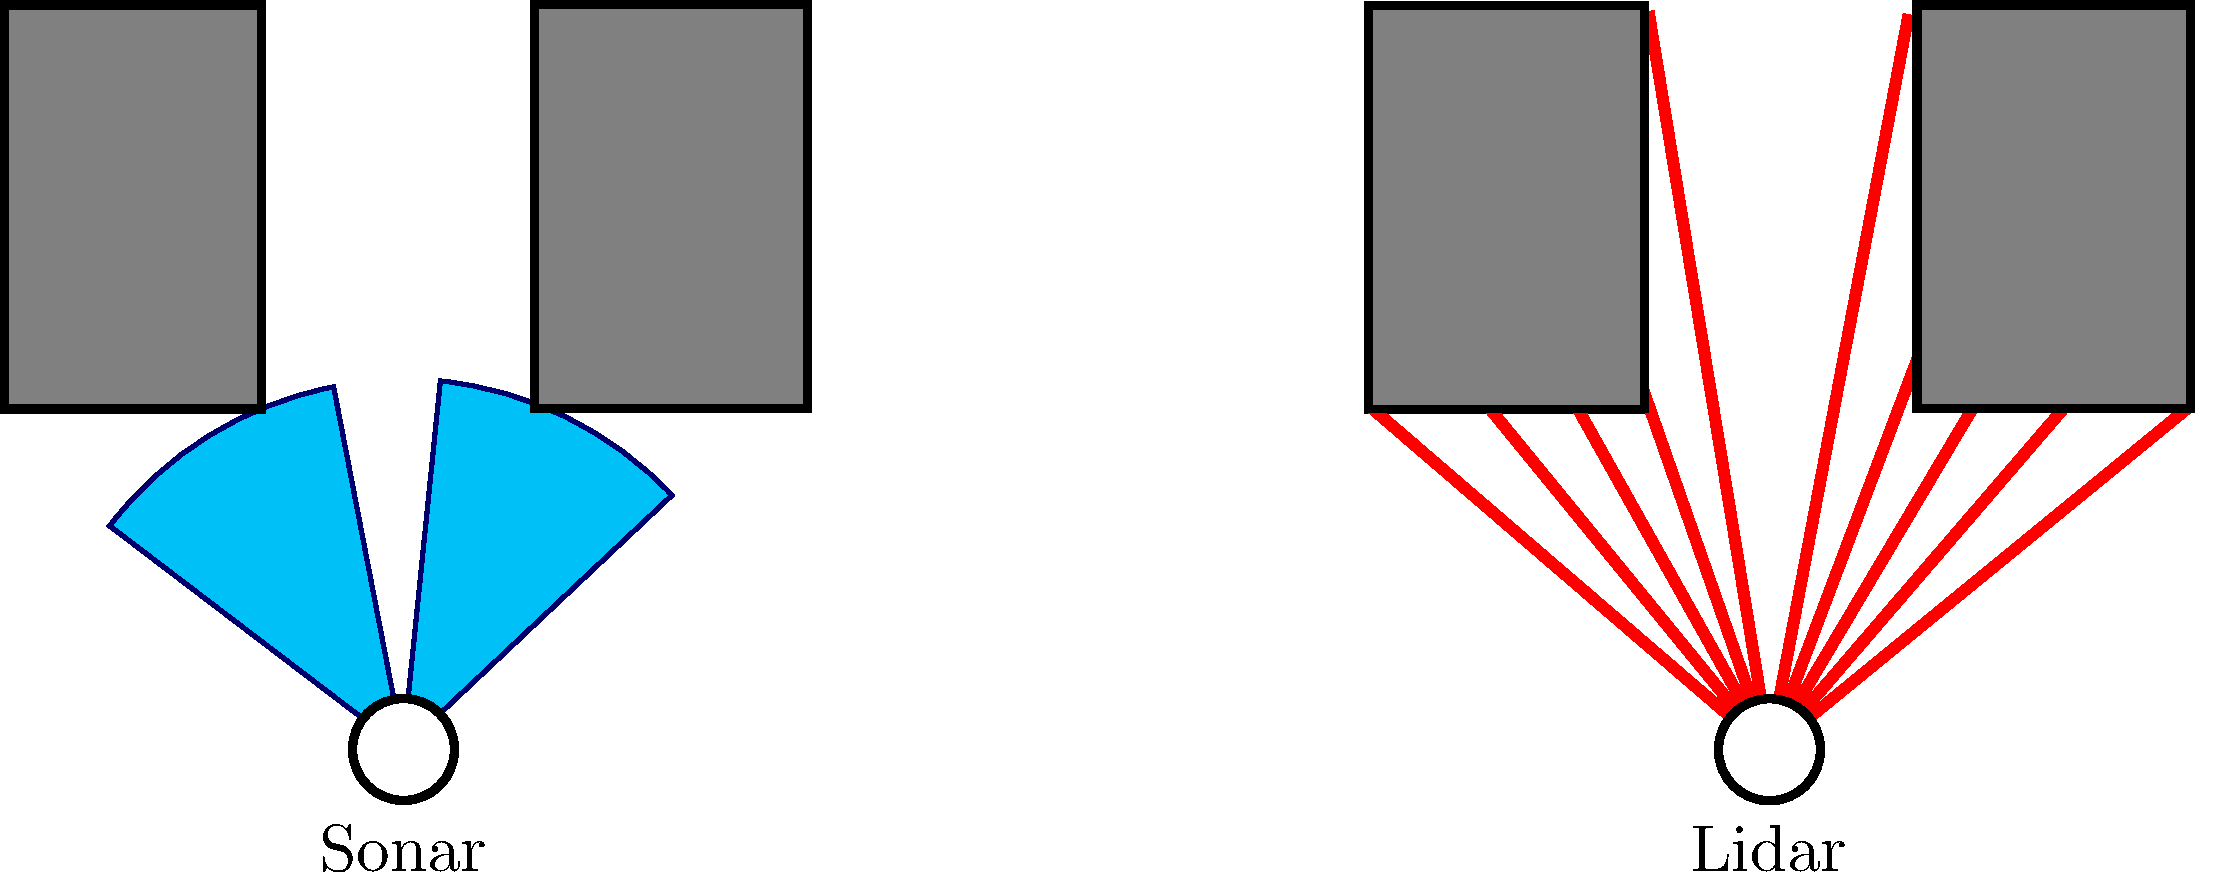
\includegraphics[width=\textwidth]{sonar_lidar1.pdf}
\caption{Sonar sensors are typically preferred when needing to detect the presence of an obstacle without
    	 needing precise position information. The location of a chair leg in the path of a robot would be
	     detected by sonar while not knowing its position in the sonar cone. Laser rangefinders have very
    	 narrow beam width, typically requiring many of them to be effective at describing an environment.
    	 If many measurements are available at high angular resolution, then they can be very effective at
    	 describing the width of narrow apertures.}\label{fig:sonar_vs_lidar1}
\end{figure}

The notion of what objects in the environment occlude a path and which do not can be viewed as a function of the gait 
(or mode of locomotion) used by the robot. If the robot is restricted to a plane, such as the case in many ground vehicles,
then an object of similar size to the vehicle could prevent traversal through that position. If the robot can also fly then
that object may not present an impediment to proceeding towards the goal.
While still not transiting through that exact position in 3D space, the 2D projection of the path onto
the plane will appear to have moved through the obstacle. This can be though of in terms of a transformation of the obstacle set according to the different
motion modalities, making a 2D planner still applicable to the problem. In Chapter~\ref{ch:crawl_gait},
a crawling gait for the Nao robot is considered which allows it to go under occlusions that it would otherwise need to plan
around.


\section{Algorithm Classifications}
Here some of the different notions common to navigation algorithms are explored. These classifications are sometimes useful
for the navigation engineer to think about as tools available to solve the navigation problem. While additional classifications
and subclassifications of algorithms can be considered, the following description is intended as a brief overview of the 
essential concepts.

\subsection{Global}
One approach to the navigation problem is to consider the entire task and configuration space of a problem when generating
a solution. For example, the task space of a robot arm might be the pose of the end effector and all of the occlusions
within that space. The configuration space would be the set of all valid joint angles that the arm can attain. Using this,
an algorithm can compute a time sequence of poses or movement commands that the robot should execute in order to bring it
from its current pose to the final pose. While this approach is ideal in the sense of generating a solution to the 
original problem, it has several practical disadvantages. One requirement of the algorithm is having a complete description 
of the task space. In many cases global knowledge of occlusions while planning is not available meaning that when new
obstructions are observed, the algorithm needs to replan the path. The other commonly encountered problem with these
algorithms is when the magnitude of the space to be planned through is so large that computing a solution cannot be done
in real-time.
% [Insert picture of global path and local directions.]
\begin{figure}
\centering
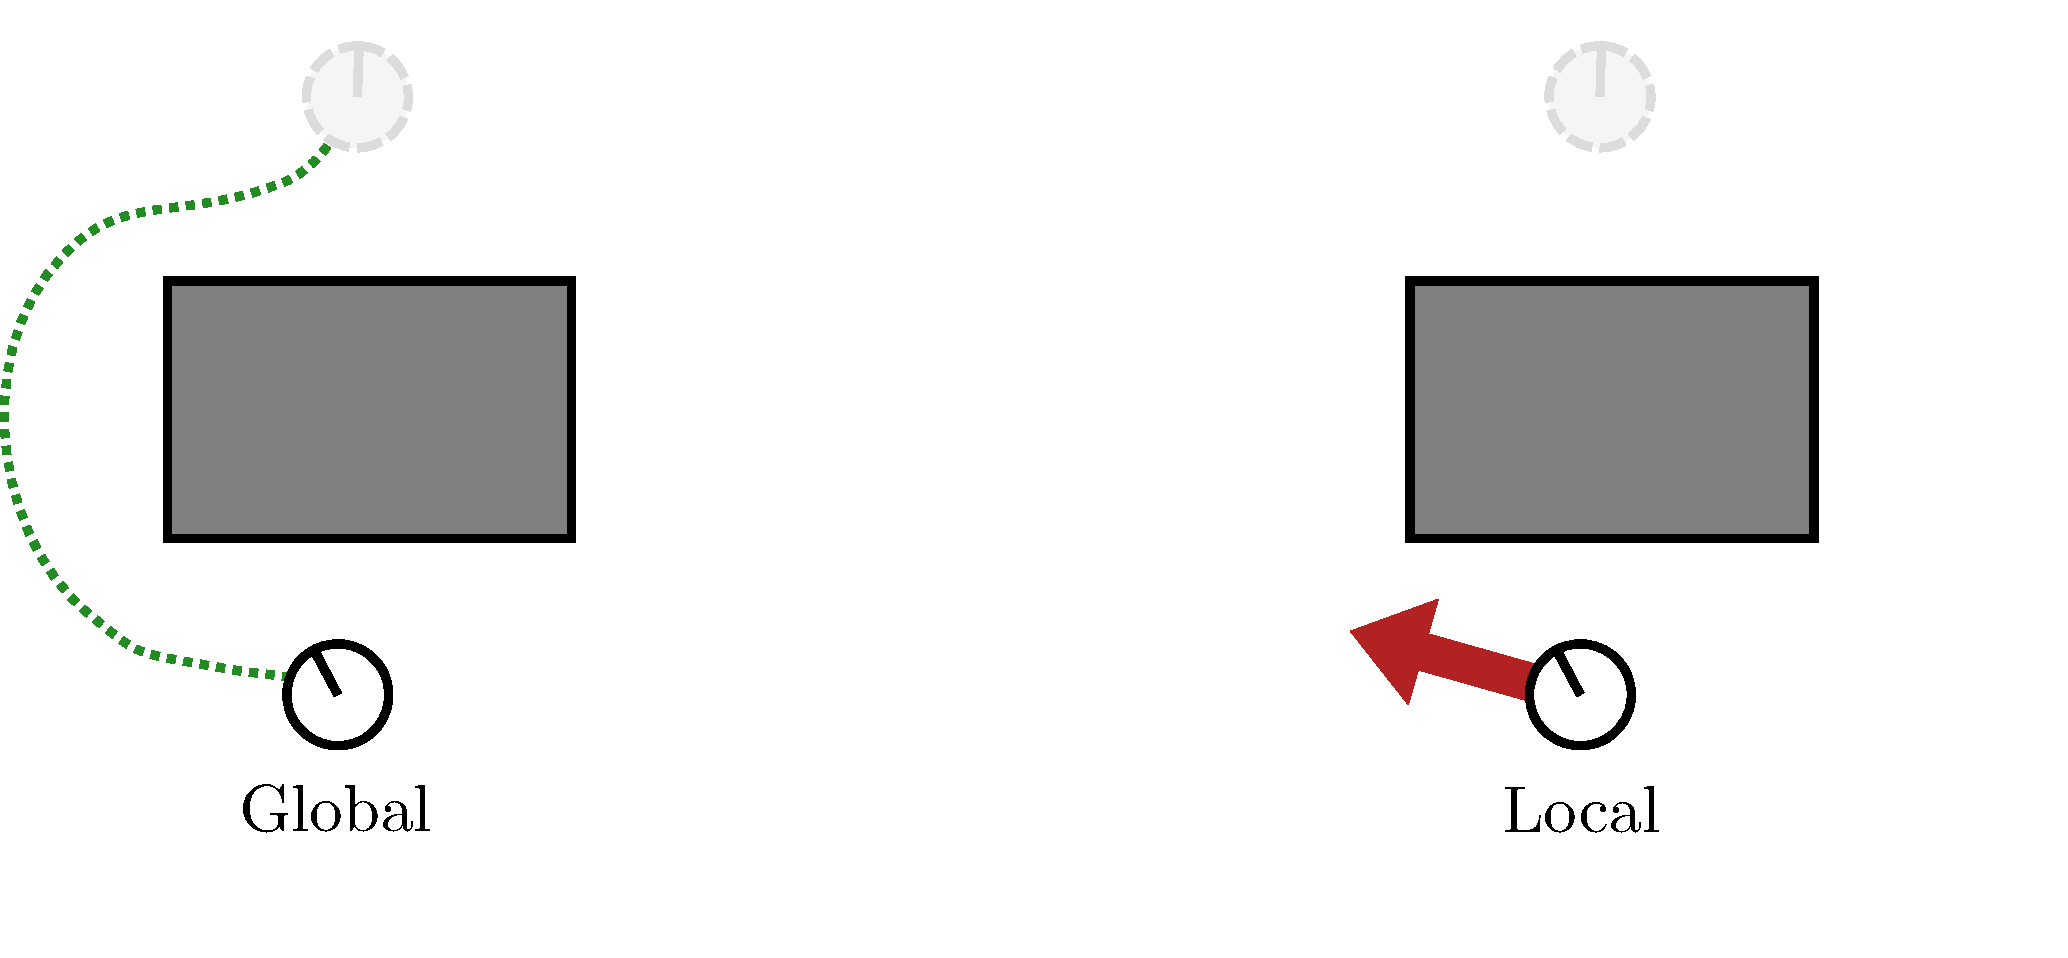
\includegraphics[width=\textwidth]{global_local1.pdf}
\caption{In global approaches, an entire path is planned to the goal before commanding the robot. In local 
         schemes, the robot is given commands calculated as a function of its position and the local environment and
	     a complete path to the goal is typically precomputed.}
\label{fig:global_vs_local1}
\end{figure}

\subsection{Local}
A different approach to the navigation problem is generating commands based only on the current information available 
or a short history about the environment. In the robot arm example, there might be a sensor such as a camera that
can detect objects that are obstructing the end effector from reaching the goal and instructs the arm to move around it.
Such algorithms usually have the advantage of being quick to compute as compared to their global counterparts because
they only have to consider a small subset of the task and configuration space. Their main disadvantage is that since they
only use such a limited amount of information, they can become trapped in local optima that do not allow the robot 
to achieve the desired pose.

%%% Continuous and Discrete %%%
\subsection{Discrete}
Orthogonal to the ideas of local and global path planning which deal with the scope of the time and space being considered
when generating navigation commands is how these spaces are represented. One way to represent the space is to break it
up into a set of discrete locations and then plan through that discretized representation. The task space for example could be divided into uniform 
spatial regions which an algorithm can consider visiting when planning a path. Alternatively, as with the robot arm example,
a finite set of movement commands can be considered and iterated through while generating a solution. 
Graph-based search algorithms such as  Dijkstra's algorithm or A* are examples of discrete solvers.
An advantage to this is that paths with complex shapes can be generated to accommodate difficult constraints. 
One point however to consider in this approach is how finely to resolve the task or configuration spaces. 
Coarser discretization can allow a solution to be computed rapidly but might miss more optimal solutions. 
% [Insert grid based path example.]
\begin{figure}
\centering
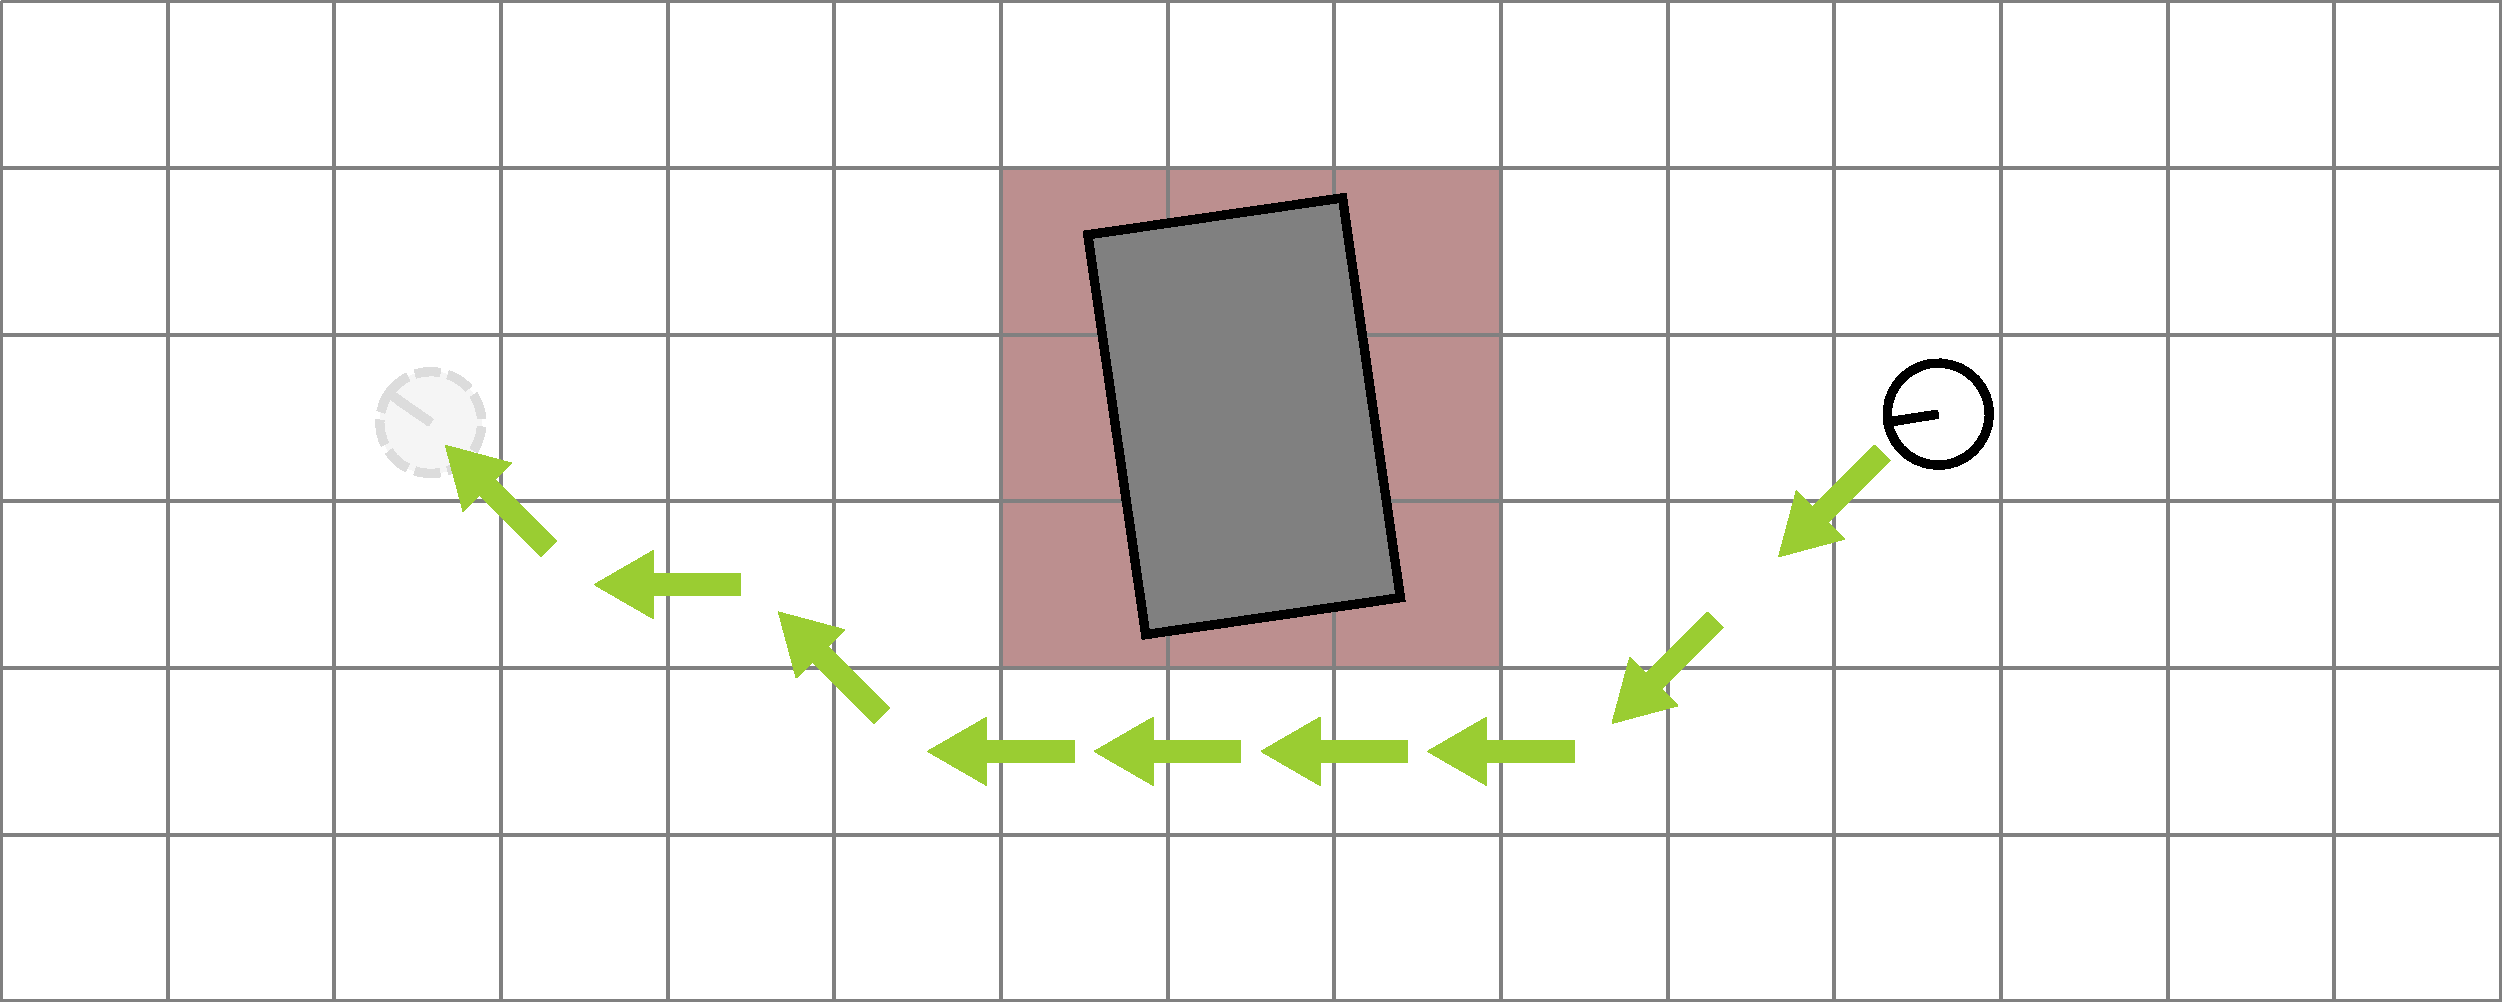
\includegraphics[width=\textwidth]{grid_world1.pdf}
\caption{The environment here is being represented as occlusions in a 
         discrete grid of locations. This allows the robot to plan through
         successive locations to the goal using graph-based techniques.}
\label{fig:grid_world1}
\end{figure}

\subsection{Continuous}
Continuous spatial representation avoids the problem of having to choose a discretization resolution. The movement commands or paths
are planned in a continuum allowing paths to take on intermediate values not available at a given discrete resolution.
Continuous representation instead has a different problem of paths needing to take on particular solution forms. A path
through the task space might be represented as a cubic spline from the current pose to the goal pose. This path has access
to the entire task space but may not be able to construct a path under complicated environments with many obstacles. Often
instead of using a single cubic, designers will use a series of cubics, the termination of one being the starting
position of the next, until the goal is reached. 
Alternatively, instead of restricting the path representation to a series of cubics, other trajectory forms can be
utilized as a library of representations such as higher-order polynomials, trigonometric functions, etc.
One example of such a planner is known as a ``maneuver-based'' planner.
% [Insert figure than shows a successful cubic spline path and a maze where you couldn't use that.]  
\begin{figure}
\centering
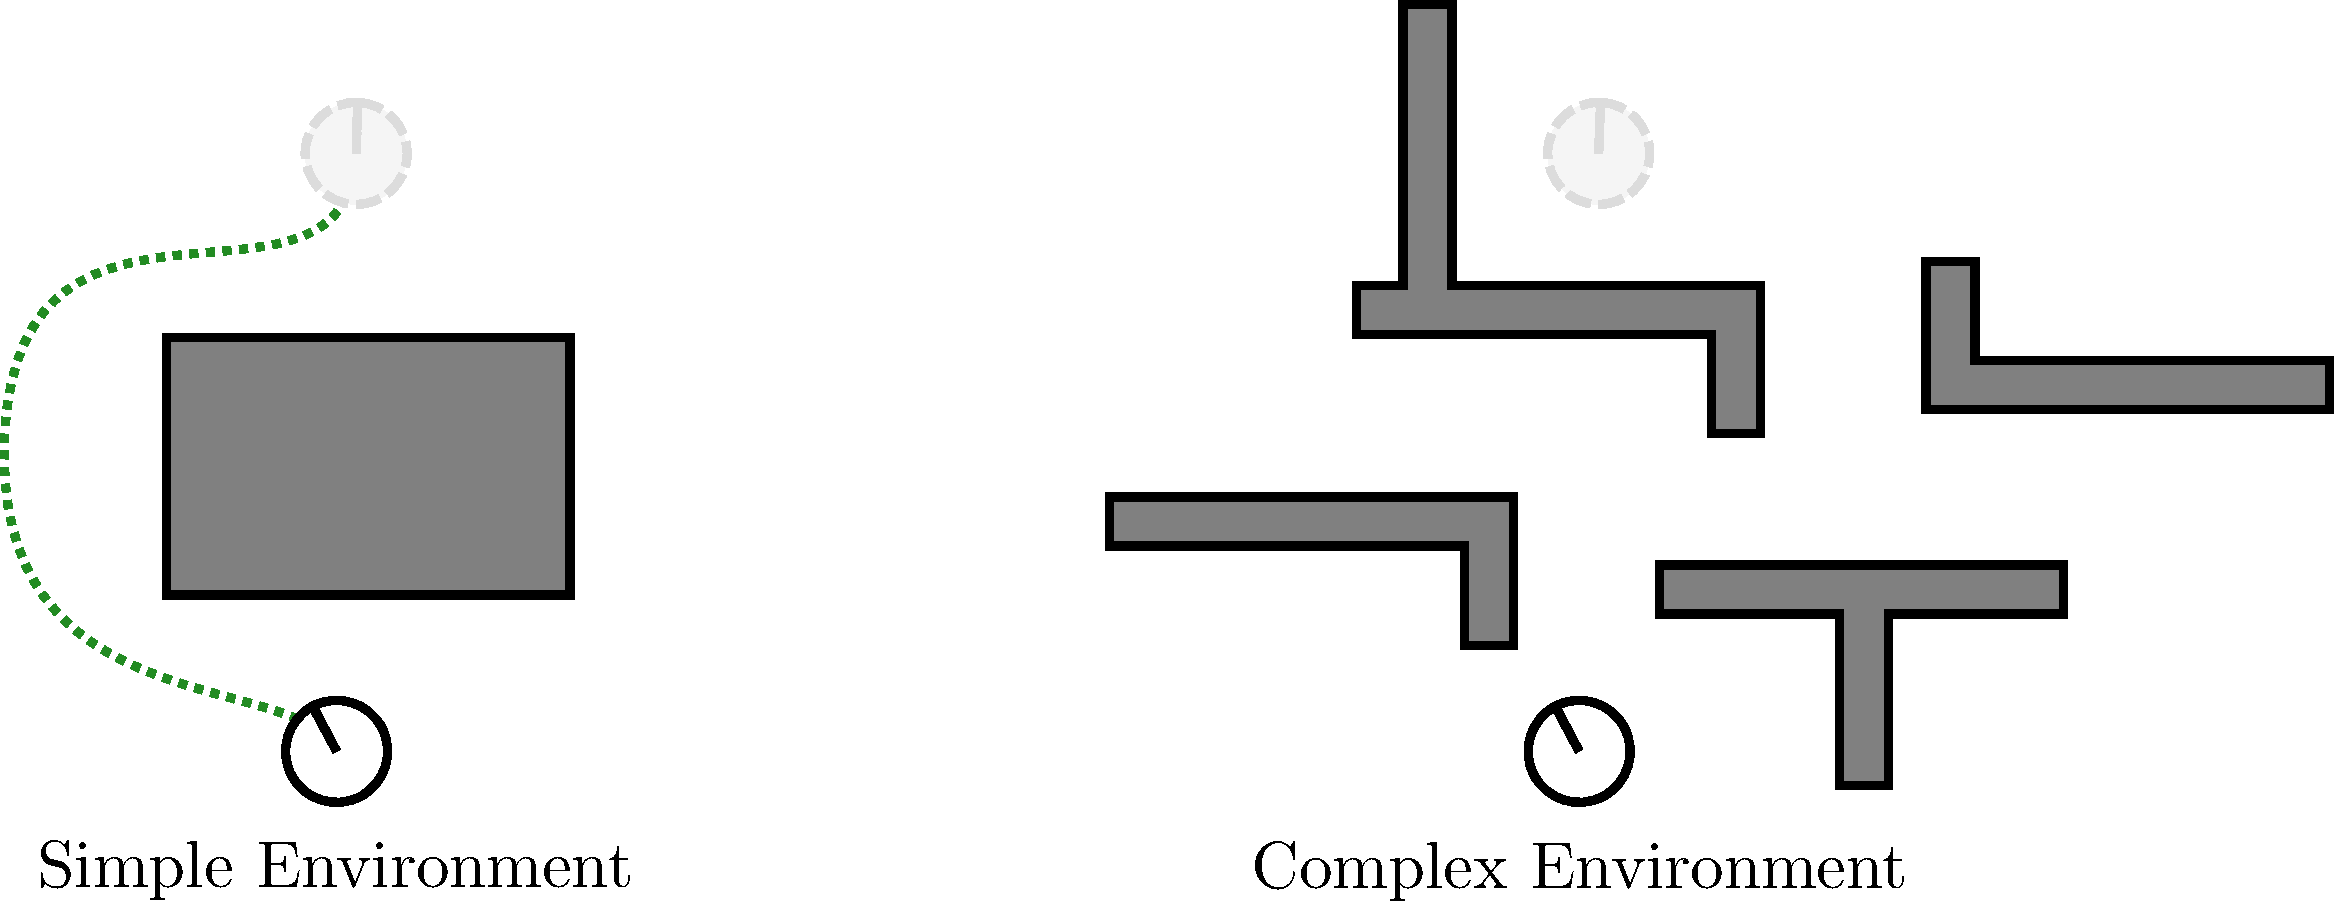
\includegraphics[width=\textwidth]{cubic1.pdf}
\caption{This figure shows two sample environments. On the left, the robot can follow a trajectory that takes
	     a cubic form and reaches the goal location. On the right, a more complicated environment is shown where a single 
	     cubic cannot describe an appropriate path.}
\label{fig:cubic1}
\end{figure}

\subsection{Composite Approaches}
In order to combine the strengths and combat the weaknesses, the above approaches are often combined to form a more robust
navigation solution. Global plans can be generated as a series of intermediate goals or way points for local planners to 
navigate towards. These way points can be planned on a coarse discrete grid that is quick to compute while low dimensional
continuous trajectories are plotted between them. Lattice planners are an example of such a composite algorithm. 
% [Show lattice plan figure.]
\begin{figure}
\centering
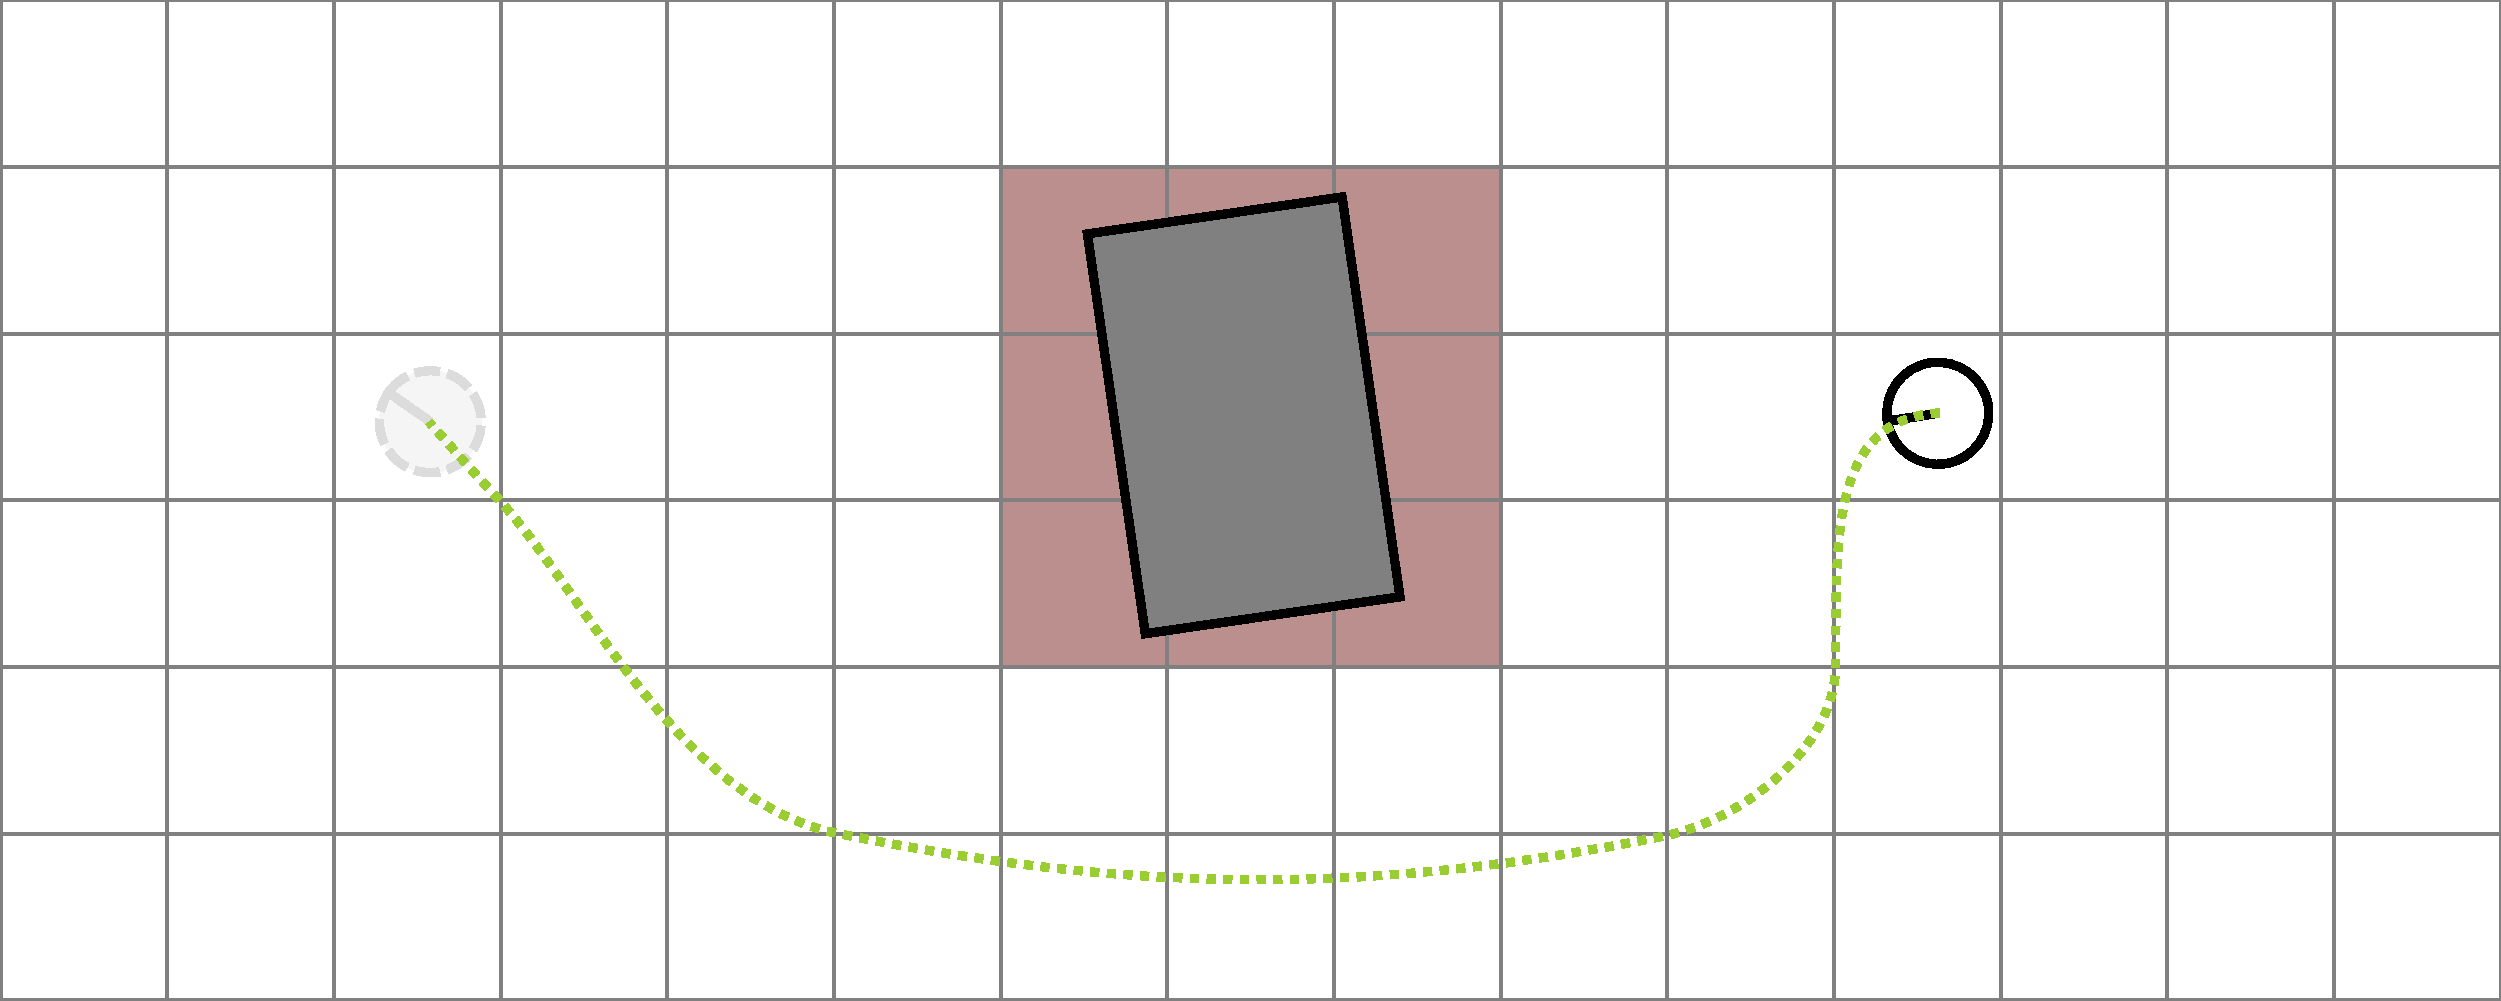
\includegraphics[width=\textwidth]{lattice1.pdf}
\caption{A lattice planner is an example of a composite discrete and continuous path planner. The planner
         first plans through a discrete grid and then designs trajectories that bring the robot from each point in the planned discrete grid to the next.}
\label{fig:lattice1}
\end{figure}

\section{Potential Fields}\label{sec:navpotfields}
Potential fields algorithms are continuous local planners. They work on the concept of modeling the robot as a sort of
charged particle (like an electron) and obstacles in the environment are modeled as having the same polarity of charge as the robot thereby producing a repulsive field pushing the robot away
from them. The goal location in is modeled as having an opposite charge to the robot and thus produces an attractive force, pulling the robot towards it. As the robot moves through
the environment, it detects objects and generates motion commands based on its range and direction. 
\begin{figure}
\centering
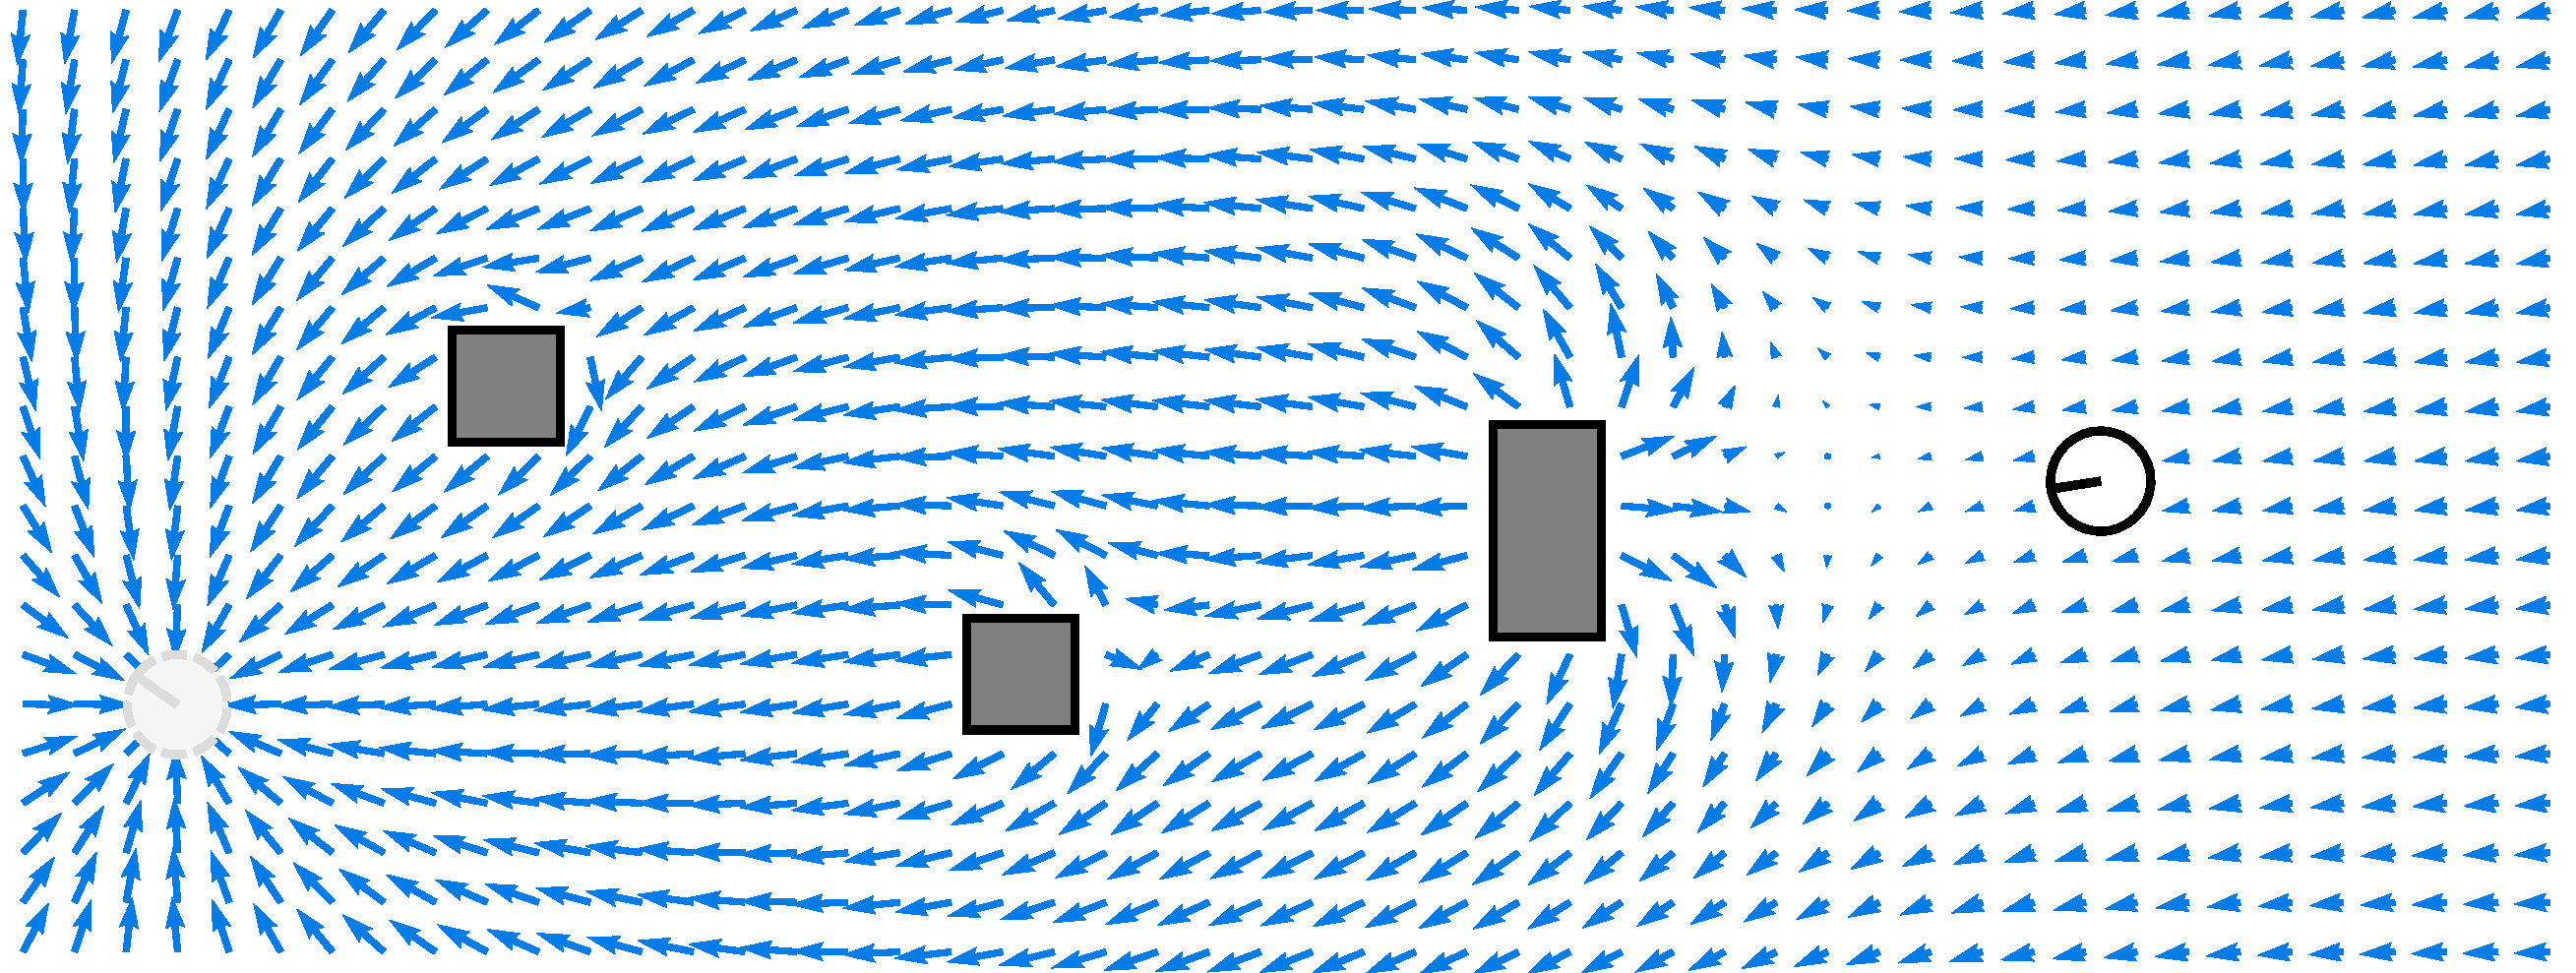
\includegraphics[width=\textwidth]{potentials1.pdf}
\caption{Visualization of potential fields idea. Objects in the environment emit a field that repels the robot
         and the goal emits an attractive field. This can be visualized as a 2D or 3D vector field.}
\label{fig:potentials1}
\end{figure}

Given a vector $x_r$ which describes the position of the robot in the task space and the positions of obstacles
$m_i$ in the set of all obstacles $M$, a force vector $f_i$ can be generated for each obstacle that describes the 
magnitude and direction of the repulsive force applied to the robot by the obstacle. The force direction
is in the opposite direction of the relative bearing of the obstacle to the robot with magnitude being inversely
proportional to the distance of the obstacle from the robot. Equation~\ref{eq:potentials_eq1} shows an example
of force vector generation.

\begin{align}
	\norm{f_i}  &= \frac{-c_i}{\norm{m_i - x_r}^\alpha}\\
	\angle{f_i} &= \angle(m_i - x_r)
\label{eq:potentials_eq1}
\end{align}

$m_i - x_r$ is the location of the obstacle relative to the robot and $c_i$ is a positive scalar used to tune force
magnitude. In some implementations, $c_i$ can be a function of the relative bearing, for example, decreasing the repulsion
effect if the obstacle is not in the direction of the goal. The parameter $\alpha$ in general can be any positive scalar
but is often picked to be 2.

For the goal seeking behavior, the equations are similar, with the direction of the force being in the direction of the 
goal, rather than away from it.

\begin{align}
	\norm{f_g}  &= \frac{c_g}{\norm{x_g - x_r}^\gamma}\\
	\angle{f_g} &= \angle(x_g - x_r)
\label{eq:potentials_eq2}
\end{align}

$x_g - x_r$ in equation~\ref{eq:potentials_eq2} is the relative location of the goal with respect to the robot and $c_g$ is some positive
tuning scalar. $\gamma$ is some positive scalar, typically 2.

The sum of these forces is used to produce a force vector $f_r$ used to command the robot away from obstacles and towards the goal
location. 

\begin{equation}
	f_r = f_g + \sum_{i = 1}^{\norm{M}} f_i
\label{eq:potentials_eq3}
\end{equation}

where $\norm{M}$ is the number of obstacles (modeled as a discrete set).

\section{GODZILA}\label{sec:navgodzila}

GODZILA (Game-theoretic Optimal Deformable Zone with Inertia and Local Approach)~\cite{Krishnamurthy07} is a local 
continuous navigation algorithm based on the potential fields idea. In contrast to some potential fields formulations
which work on the range and bearing of objects in the environment, GODZILA uses the sensor information about occlusion
locations directly in order to formulate navigation commands. It is a memoryless algorithm and does not attempt to
build a map of the environment making it very lightweight in terms of both computation and memory. It can be implemented
on a variety of vehicles and is suited for the cases where a low computational power microcontroller is utilized.
It has three components which are an optimization cost, a straight line planner, and a stochastic local minima escape strategy.

Figure~\ref{fig:godzila_setup1} illustrates the key variables in the formulation.
\begin{figure}
\centering
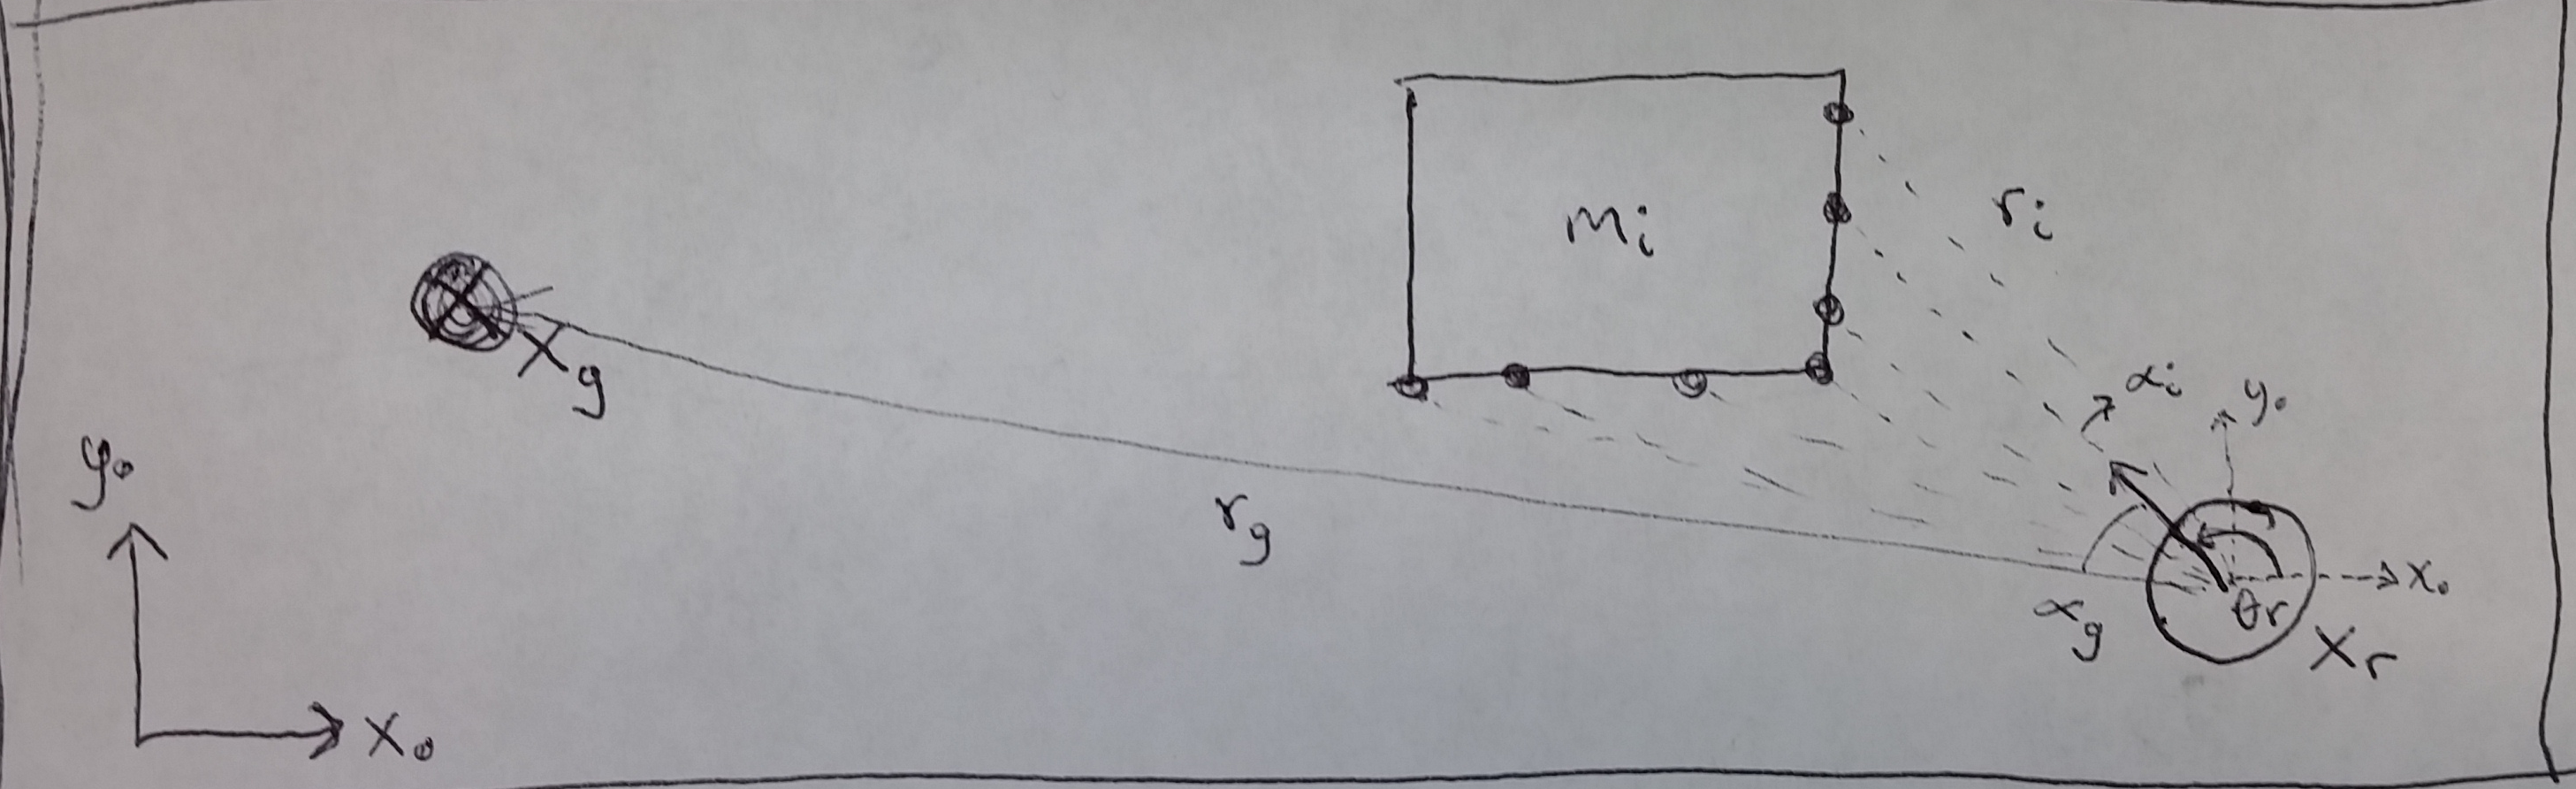
\includegraphics[width=\textwidth]{godzila_rough1.png}
\caption{Illustration of various variables utilized in GODZILA\@. Range and bearing of the goal relative to the robot are required
         as well as being able to take range measurements to occlusions and knowing the relative bearings of these measurements.}
\label{fig:godzila_setup1}
\end{figure}

Taking a 2D example of the application of the GODZILA algorithm, we have the following terms:

\begin{description}
	\item[$x_0$] is the x-axis of the inertial frame.
	\item[$y_0$] is the y-axis of the inertial frame.
	\item[$x_r$] is the (x,y) location of the robot in the inertial frame.
	\item[$\alpha_r^\prime$] is the new heading the robot should be commanded to in the robot frame.
	\item[$x_g$] is the (x,y) location of the goal in the inertial frame.
	\item[$r_g$] is the range to the goal relative to the position of the robot.
	\item[$\alpha_g$] is the bearing to the goal location relative to the orientation of the robot.
	\item[$z_i$] is the $i^{th}$ sensor measurement made by the robot which includes range and bearing to an occlusion.
	\item[$r_i$] is the $i^{th}$ range measurement to an occlusion relative to the position of the robot.
	\item[$\alpha_i$] is the bearing angle to the $i^{th}$ sensor measurement.
\end{description}

In this formulation, it is assumed that there is some mechanism to allow the robot to get an estimate of the relative
range and bearing to the goal location $r_g$ and $\alpha_g$ and that the robot has some sensors that can provide range
and bearing to occlusions in the environment.

\subsection{Optimization Formulation}\label{subsec:navoptimization}
The formulation of the GODZILA algorithm is in terms of an optimization cost. The goal of the algorithm is to bring the robot
towards the goal while preventing it from colliding with obstacles. With this intuition the cost function has three components:

\begin{enumerate}
	\item $J_1(\alpha_r^\prime)$ which rewards goal seeking by penalizing directions other than those towards the goal.
	\item $J_2(\alpha_r^\prime)$ which penalizes directions towards occlusions.
	\item $J_3(\alpha_r^\prime)$ which dampens oscillations by penalizing changes in heading.
\end{enumerate}

The sum of these terms produces the cost function to be minimized:

\begin{equation}
	\min_{\alpha_r^\prime} \sum_{i = 1}^3 J_{i}(\alpha_r^\prime)
\end{equation}

where $\alpha_r^\prime$ is the heading direction the robot should travel in order to minimize the cost function. 
$J_1(\alpha_r^\prime)$ takes on the form of:
\begin{equation}
	J_1(\alpha_r^\prime) = g_{11}(r_g) f_{11}( \norm{\alpha_r^\prime - \alpha_g} ).
\end{equation}

$g_{11}$ is a class-${\cal L}$ function meaning that it is continuous and monotonically non-increasing which maps $[0, \infty) \mapsto [0,\infty)$
and $f_{11}$ is a class-${\cal K}$
function meaning it is monotonically non-decreasing which maps $[0, \infty) \mapsto [0,\infty)$. 
The intuition here is that $f_{11}$ produces a higher cost in proportion to how much the direction command $\alpha_r^\prime$ differs from the goal direction.
$g_{11}$ conversely reduces the cost if the range to the goal is large. The idea being that the farther from the goal the robot is, then being oriented
towards the goal becomes less of a priority. 

$J_2(\alpha_r^\prime)$ takes on the form:
\begin{align}
	J_2(\alpha_r^\prime) &= J_{2_{{\cal I}_1}}(\alpha_r^\prime) - J_{2_{{\cal I}_2}}(\alpha_r^\prime) \label{eq:j2}\\
	J_{2_{{\cal I}_1}}(\alpha_r^\prime) &= \sum_{i \in {\cal I}_1} g_{21}(r_i)\Big [ g_{22}(\norm{\alpha_g - \alpha_i}) + g_{23}(\norm{\alpha_i}) \Big ] g_{24}( \norm{\alpha_r^\prime - \alpha_i}) 
	\label{eq:j2_i1}\\
	J_{2_{{\cal I}_2}}(\alpha_r^\prime) &= \sum_{i \in {\cal I}_2} f_{21}(r_i) g_{25}(\norm{\alpha_g - \alpha_i}) g_{26}( \norm{\alpha_r^\prime - \alpha_i}) \label{eq:j2_i2} 
\end{align}

Equation~\ref{eq:j2} has two components to it, separated by the membership of the sensor measurements $z_i$ to one of two sets. 
The first is the set of all range measurements $r_i$ whose value falls below some positive scalar $r_c$ are put into a set ${\cal I}_1$. 
The second set is the remaining range measurements, which are necessarily greater than $r_c$, placed into set ${\cal I}_2$. 
This threshold distance $r_c$ is picked such that if the occlusion is farther away than it, the robot does not need to be concerned with avoiding it.
% J1_I1 = Go away from occlusions that are close to me. Avoid more if they are near my direction of travel or if they are in the direction of the goal.
Equation~\ref{eq:j2_i1} is concerned with the occlusions that need to be avoided, and has four class-$\cal L$ functions $g_{21}, g_{22}, g_{23}, g_{24}$ 
associated with it. The first three $g_{21}, g_{22}, g_{23}$ act as gains that the control variable $\alpha_r^\prime$ in function $g_{24}$ must attenuate.
$g_{21}$ says that if the range $r_i$ to the occlusion is small, then the cost of orienting in that direction is high.
$g_{22}$ amplifies this effect if the direction to the occlusion $\alpha_i$ is in the same direction of the goal $\alpha_g$.
$g_{23}$ also amplifies $g_{21}$ if the direction of the occlusion is similar to the heading direction of the robot.
% J1_I2 = Go towards occlusions that are far away and in the direction of the goal.
Equation~\ref{eq:j2_i2} deals with the case where the occlusions can be approached. It has one class-${\cal K}$ function $f_{21}$ and two
class-${\cal L}$ functions $g_{25}$ and $g_{26}$. $f_{21}$ and $g_{25}$ act as gains on the controlled function $g_{26}$.
$f_{21}$ promotes moving in the direction of ranges that are large and $g_{25}$ promotes moving in the direction of occlusions
that are in a similar direction to the goal direction. 

The final term $J_3(\alpha_r^\prime)$ is a class-${\cal K}$ function that penalizes changes in direction.

\begin{equation}
	J_3(\alpha_r^\prime) = f_{31}(\norm{\alpha_r^\prime})
	\label{eq:j3}
\end{equation}

This term is present to prevent high frequency oscillations and is analogous to giving the robot a physical inertia.
All of the functions $f_{11}, f_{21}, f_{31}, g_{11}, g_{21}, g_{22}, g_{23}, g_{24}, g_{25}, g_{26}$ in the optimization are tunable by the designer but
it was noted in~\cite{Krishnamurthy07} that in the case where the controlled functions $f_{11}, g_{24}, g_{26}, f_{31}$ are 
chosen to be quadratic, the optimization problem can be solved in closed form producing the solution seen in equation~\ref{eq:closed_form1}.

\begin{align}
	\alpha_r^\prime &= \frac{\alpha}{\norm{\alpha}} \label{eq:closed_form1} \\
	\alpha &= \alpha_1 + \alpha_2 + \alpha_3 + \alpha_4 \label{eq:closed_form2}
\end{align}

The four terms in equation~\ref{eq:closed_form2} correspond to terms arising from the four optimization terms $J_1(\alpha_r^\prime), J_{2_{{\cal I}_1}}(\alpha_r^\prime), J_{2_{{\cal I}_2}}(\alpha_r^\prime), J_3(\alpha_r^\prime)$.
They are expanded in equations~\ref{eq:closed_form3}-\ref{eq:closed_form6}.

\begin{align}
	\alpha_1 &= \overline f_{11}g_{11}(r_g)\alpha_g \label{eq:closed_form3} \\
	\alpha_2 &= - \overline g_{24} \sum_{i \in {\cal I}_1} g_{21}(r_i)\Big [ g_{22}(\norm{\alpha_g - \alpha_i}) + g_{23}(\norm{\alpha_i}) \Big ] \alpha_i
					\label{eq:closed_form4} \\
	\alpha_3 &= \overline g_{26} \sum_{i \in {\cal I}_2} f_{21}(r_i) g_{25}(\norm{\alpha_g - \alpha_i})\alpha_i \label{eq:closed_form5} \\
	\alpha_4 &= \overline f_{31} \alpha_r \label{eq:closed_form6}
\end{align}

The solutions to the equations reuse functions $f_{21}, g_{11}, g_{21}, g_{22}, g_{23}, g_{25}$ as they are not functions of $\alpha_r^\prime$ and produce constant versions
of $f_{11}, f_{31}, g_{24}, g_{26}$ as $\overline f_{11}, \overline f_{31}, \overline g_{24}, \overline g_{26}$ in the direction of their respective directions
$\alpha_g, \alpha_i \forall i \in {\cal I}_1, \alpha_i \forall i \in {\cal I}_2, \alpha_r$ where $\alpha_r = [1,0]^T$ representing the current heading of 
the robot in the vehicle frame.

The resultant $\alpha_r^\prime$ is typically commanded as an angular rate $\dot \alpha_r^\prime$ according to the angular velocity bandwidth of the vehicle.

Finally, the linear velocity is still to be commanded. A good choice for this function is of the form:
\begin{equation}
	v_r = f_v(\min(R))g_v(\dot \alpha_r^\prime)
\label{eq:linear_velocity1}
\end{equation}

where $R$ is the set of all range measurements, $f_v$ is a class-${\cal K}$ function and $g_v$ is a class-${\cal L}$ function. 
This reduces the speed of the vehicle when it is in close proximity to occlusions or if it is commanded to a high angular rate.
Slower speeds near obstacles makes it less likely that the vehicle will collide with them. Slower speeds at times when the robot is commanded to
high angular rates helps reduce the distance the robot travels in a previously commanded direction before completing a new 
turn command.

\subsection{Straight Line Planner}

If at some point during the navigation of the vehicle to the goal the straight line path from the robot to goal becomes
unobstructed, it follows that the robot should proceed directly to the goal according to this path. This is sensible, but
can bring the robot in close proximity to obstacles. It is therefore desirable to preserve the obstacle avoidance properties
of the optimization procedure from Chapter~\ref{subsec:navoptimization}. This procedure is especially useful in situations where the width of the aperture between 
occlusions to the goal approaches the width of the robot where the obstacle avoidance behavior might deter traversal to the goal. 
This can be achieved by prescribing intermediate goal locations
according to:
\begin{equation}
	\hat x_g(t) = (1 - \lambda(t - t_0)) x_r + \lambda (t - t_0) x_g
\label{eq:line_path1}
\end{equation}

where $\lambda(\tau)$ is a monotonically increasing function that maps $[0, T_f] \mapsto [0,1]$ with $T_f$ being some 
amount of time allowed for the vehicle to reach the goal location. The length of time the planner is active is $T_f$.
If the robot has not reached the goal in this time but again has a straight line path to the goal the planner is allowed
to restart.

\subsection{Escape Strategy}\label{subsec:escape_strategy}

While the inertial term provided by\ref{eq:j3} is intended to reduce high frequency oscillations and backtracking that might
trap the robot in small corners, it is not enough to account for degenerate cases such as those shown in Figure~\ref{fig:trap1}.

\begin{figure}
\centering
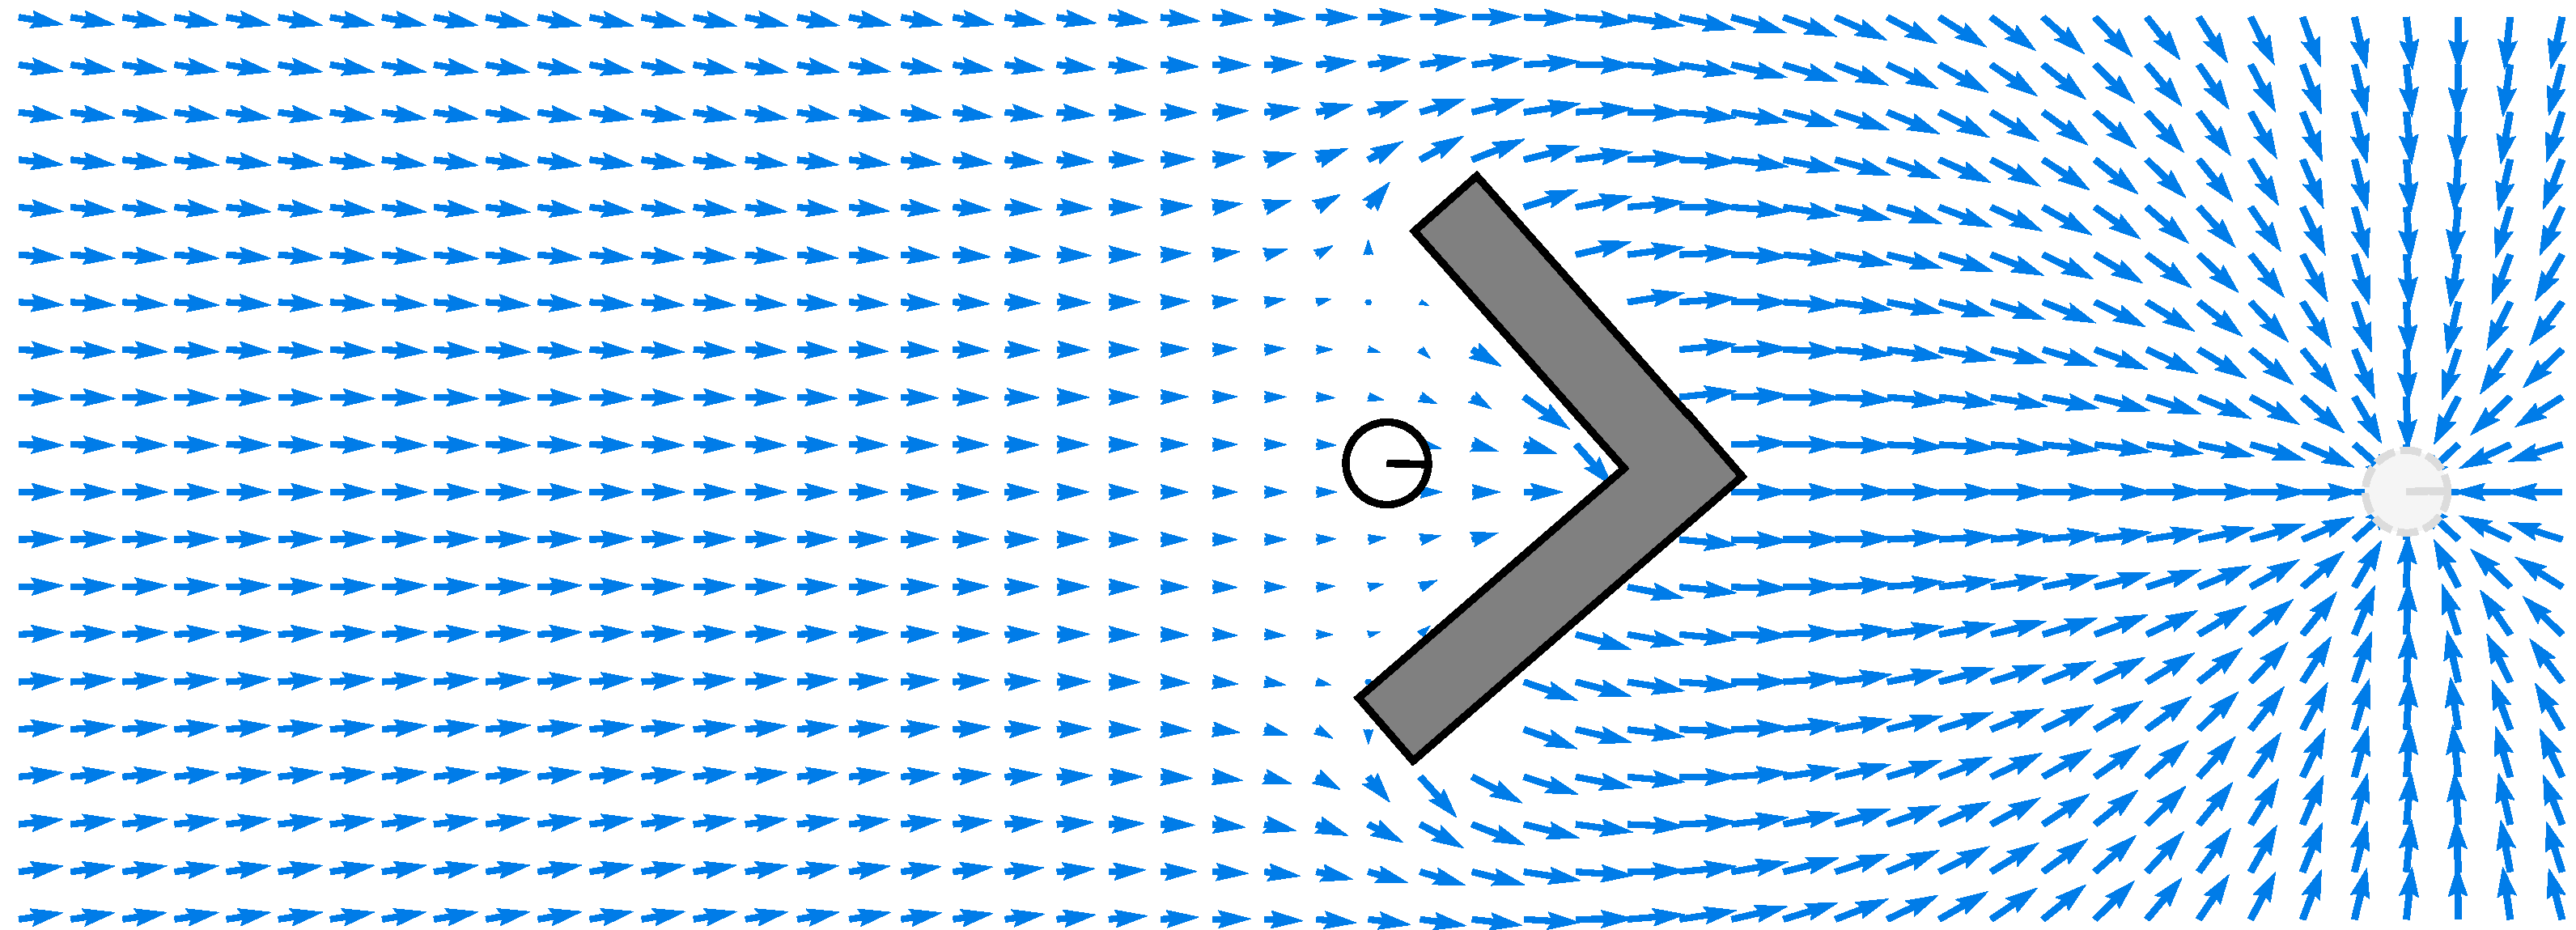
\includegraphics[width=\textwidth]{navtrap1.pdf}
\caption{A degenerate case where the attractive force of the goal combines with the repulsive force of the wall producing a local optima
	     where the robot gets trapped.}
\label{fig:trap1}
\end{figure}

In such scenarios, an effective strategy to escape such traps is to randomly assign an alternate goal position $x_{rand}$
that will allow the robot to escape the local minima and proceed to the goal. The distance to $x_{rand}$ from the robot
is typically selected to be smaller than the distance to the nearest occlusion $\min(R)$. After some fixed time, the
goal position is set back to $x_g$. If the trap condition is detected multiple times then the next escape procedure is
repeated that many times before being restored to $x_g$. One possible method to detect a trap condition is to integrate
a sliding window of vehicle linear velocities $v_r$ and if those values integrate to a position close to zero then is is likely
that the robot has encountered a trap condition. It is shown in~\cite{Krishnamurthy07} that with all of these mechanisms the position of the robot 
$x_r$ will converge to $x_g$ in finite time with probability 1.

	
%%%%%%%%%%%%%%%%%%%%%%%%%%%%%%%%%%%%%%%%%%%%%%%%%%%%%%%%%%%%%%%%%%%%%%%%%%%%%%%%%%
%%% Crawl Gait
%%% 
%%%
%%%%%%%%%%%%%%%%%%%%%%%%%%%%%%%%%%%%%%%%%%%%%%%%%%%%%%%%%%%%%%%%%%%%%%%%%%%%%%%%%%
\chapter{Humanoid Crawl Gait} \label{ch:crawl_gait}

Using the Nao platform, crawling gaits applicable to humanoid robots was explored. 
Not only is crawling a more stable gaiting strategy than walking, but it gives the robot access to areas
of the environment that are inaccessible via walking alone. A low-profile laterally symmetric crawl gait is described, 
modeling the robot as a closed-chain manipulator with pseudo-static dynamics. This gait was parameterized on 
three joint variables and optimized using a cubic splines approach via a genetic algorithm.

As was described in Chapter~\ref{ch:navigation}, the gaiting modality directly affects the navigation strategy.
By selecting the appropriate gaiting strategy, the robot can modify its movement to achieve a commanded goal.
This modified movement also modifies which environmental objects present as obstacles.
Expanding the library of gaits legged robots have access to allows robots to be increasingly more capable
and applicable to a wider range of scenarios.

\section{Humanoid Crawling}

Unlike walking and running which enjoy precise definitions, crawling seems to only have a subjective notion.
\cite{Dudek2000} asserts that crawling is a statically stable walk. This definition is problematic
as bipedal gaits can be statically stable but would not
be classified as crawling. In addition to this, soldiers performing the high army crawl \cite{armyfieldmanual2008} can be seen to
perform this motion very quickly which introduces a dynamic component to the crawl.
The standard or baby crawl is described as using one's hands and knees to produce forward motion.
In contrast to this, crawls such as the leopard, tiger, bear, and crab use hands and feet to produce
forward motion and the low army crawl uses the hands to drag and one leg to push the body across the ground.
Such diversity in crawling motion makes it difficult to differentiate a crawl from a statically stable
quadrupedal gait that uses something other than the end effectors to interact with the environment.
Despite this, the presented gait produces a motion that many would associate with humanoid crawling.

\subsection{Nao Crawling Limitations}

A primary limitation to the gaits that can be produced by the Nao is the limited number of degrees of freedom (DoF) of the platform
in contrast to the large number of DoF present in humans. While the Nao has 25 DoF, the human body has 244 \cite{zatsiorskybiomechanics}.
The human arm and leg each have 7 DoF while the Nao's arms and legs each have 5. 
Nao's hips have one more degree of freedom, called Hip Yaw-Pitch, which turn the legs together at an angle. 
Figure~\ref{fig:nao_hips_legs1} illustrates this degree of freedom more clearly. 
The rest of the DoF of the Nao are in the hands and neck. 
Notably, Nao has no back joint. This prevents the gait designer from prescribing a twisting motion for use in the crawl gait.
These limits in motion preclude the execution of any gaits that require lateral twisting or sagittal arching.

\begin{figure}
	\vspace*{-0.07in}
	\centerline{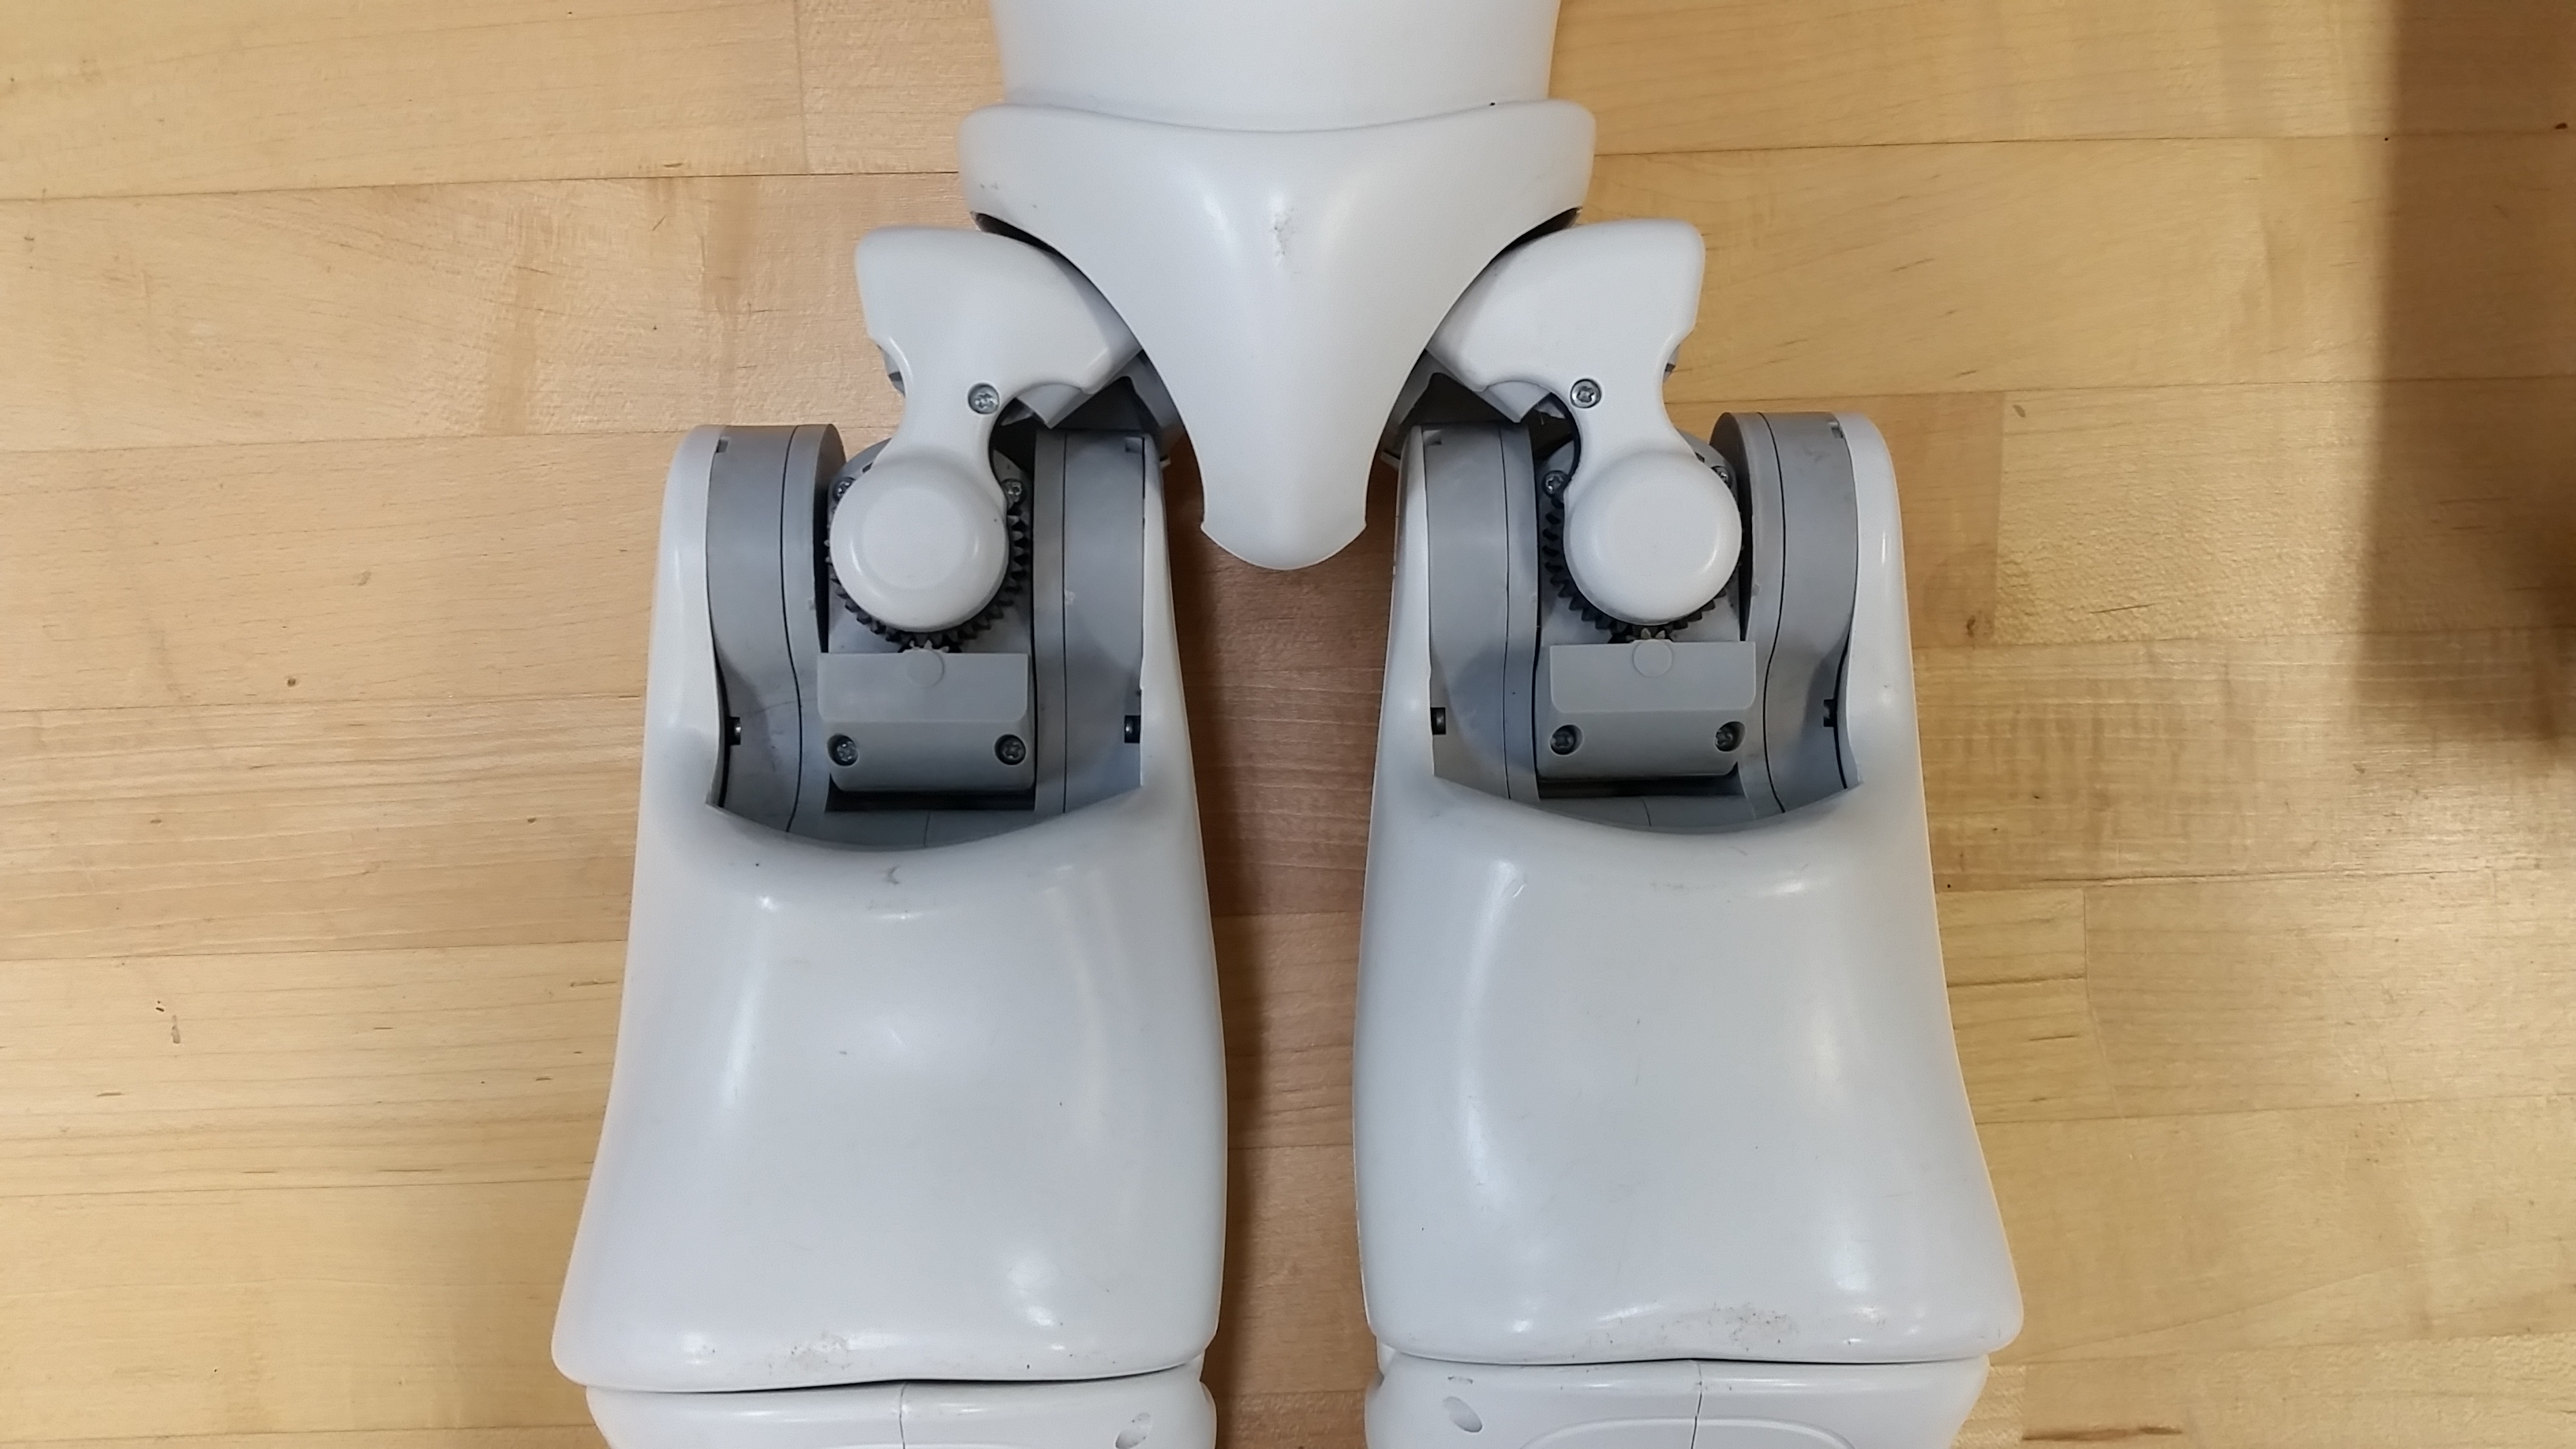
\includegraphics[width=0.395\textwidth]{nao_legs_together1.png}
				\includegraphics[width=0.5\textwidth]{nao_legs_spread1.png}
				}
	\caption{The pane on the left shows the leg configuration of the Nao when the Hip Yaw-Pitch DoF is fully turned in.
				The right pane show the leg configuration when the Hip Yaw-Pitch is fully turned out. 
				The legs are mechanically linked, making the amount of Hip Yaw-Pitch equal for each leg.}
	\label{fig:nao_hips_legs1}
	\vspace*{-0.2in}
\end{figure}

\section{Projected Profile Humanoid Crawl Gait}

The crawling gait presented in this thesis is based on viewing the humanoid form as a set of manipulators on the
sagittal plane. Figure~\ref{fig:nao_sideview1} illustrates this concept.
When the robot is laying in the prone position, it necessarily makes contact with the ground. If we then view the robot
from the side (looking at the sagittal plane) we can model it as a planar kinematic chain. If the chest and knees
are making contact with the ground, then the arms from the shoulder joint to the hand, and the legs from the knees to the
toes are free to move without affecting the rest of the body. This produces two open chain manipulators. In the case of the Nao, each has two degrees
of freedom in the sagittal pane, allowing the hands and feet to move independently.
\begin{figure}
	\centering
	\includegraphics[width=\textwidth]{nao_pp_sagittal_view2.pdf}
	\caption
	{Illustration of Projected Profile concept. Both panes show the saggital view of the Nao with a schematic representation of the kinematics. 
	In the top view, the robot appears as two open chain manipulators. In the bottom view, the robot appears as one closed chain manipulator.}
	\label{fig:nao_sideview1}
\end{figure}

If the elbows and toes are placed on the ground, then the body from the toes to the elbow can be viewed as a closed chain manipulator.
This allows the joints to work together to move the center of mass. Kinematically, these two phases share two common configurations.
The first configuration is when the elbow is at full extension and the toes touching the knees. We will call this the ``extension" configuration.
This can be viewed as the robot reaching forward. The second is when the elbow is at full flexion and the ankles at extension.
We will call this ``compression".
This can be viewed as the robot having pulled itself forward. These motions can then be combined
to produce a full gait.

Using the Nao robot as an example, Figure~\ref{fig:nao_phases1} shows the full gaiting sequence.
The robot initializes itself in the open chain configuration. From this, it can position
its end effectors (the toes and elbows) into the first common configuration ``extension". Next, the robot is in the closed chain 
configuration in which it can transport its center of mass forward until it reaches the ``compression" configuration. Finally the robot
is again in the open chain configuration and the cycle can start again.

\begin{figure}%[!th]
	\centerline{\includegraphics[width=0.5\textwidth]{White_Background/1_onBellyBegin.png}
				\includegraphics[width=0.5\textwidth]{White_Background/2_extension.png}
				}

	\vspace*{0.05in}

	\centerline{\includegraphics[width=0.5\textwidth]{White_Background/3_apex.png}
				\includegraphics[width=0.5\textwidth]{White_Background/5_onBellyEnd.png}
				}
	\caption{The above sequence shows the motion segments and robot postures in the crawl gait. 
				The upper left pane shows the initial open chain configuration. The upper right
				pane moves the robot to the ``extension" configuration. The lower left
				shows the ``compression" configuration. Finally, the lower right shows the 
				robot, having translated forward, once again in the open chain configuration.
				A 6-inch marker is shown in the background as a length scale reference.}
	\label{fig:nao_phases1}
\end{figure}

The gait is laterally symmetric. 
If we actuate the joints at an appropriate rate, dynamic effects from the robot's motion do not become a significant factor.
As detailed in Chapter~\ref{ch:results_crawl_gait}, this gait can be performed on the Nao at a speed of 1 ft every 6 to 8 seconds. 
The wide surface area of the forearm provides a high coefficient of friction against slipping and the small surface area of
the toes can act as a point of high pressure which can dig into soft surfaces such as carpets.
The gait is statically stable in the sense that the robot's motion can be paused at any point and the robot will maintain that pose.
The gait does not depend on the robot
sliding along the surface nor does it highly depend on surface friction to pull the robot forward.
The gait has a very low profile. The highest point on the robot during the gait (which is the top of the head)
is about 8 inches off of the ground. In contrast, during walking, the Nao robot stands 23 inches tall.

\subsection{Open Chain Kinematics}
The Projected Profile crawl gait has two kinematic configurations: open chain and closed chain. In the open chain
configuration, the robot acts as two independent planar manipulators. 
Each manipulator has two degrees of freedom as can be seen in Figure\ref{fig:open_chain1}.

\begin{figure}
	\centering
	\includegraphics[width=\textwidth]{stick_open_chain1.pdf}
	\caption
	{Simplified kinematic model of the sagittal projection of the open chain configuration.
	The manipulator on the left represents the tibia-foot chain. The manipulator on the right
	represents the humerus-forearm chain. The origin of the knee and shoulder are represented as 
	having a z-axis offset because the knee and chest of the robot have heights that raise their 
	origins.}
	\label{fig:open_chain1}
\end{figure}

With the Nao facing downwards, the feet towards the origin and the head in the positive x direction, 
the forward kinematics for each manipulator are described by:
\begin{align}
	x &= x_0 + l_1 cos(\theta_1) + l_2 cos(\theta_1 + \theta_2) \\
	z &= z_0 + l_1 sin(\theta_1) + l_2 sin(\theta_1 + \theta_2)
\end{align}
where $x_0$ and $z_0$ are the superior and posterior offsets with respect to the global frame, respectively. $l_1$ is the length of the
humerus/tibia, $l_2$ is the length of the forearm/foot, $\theta_1$ is the angle subtended by the 
shoulder/knee and the x-axis, and $\theta_2$ is the angle subtended by the ankle/elbow and the x-axis of the humerus/tibia.

The solutions to the inverse kinematics problem can be seen as:

\begin{align}
	\theta_2 &= \cos^{-1} \left (\frac{(x - x_0)^2 + (z - z_0)^2 - l_1^2 - l_2^2}{2 l_1 l_2} \right ) \label{eq:open_fk_eq1}\\
	\theta_1 &= 2 \tan^{-1} \left (\frac{-B \pm \sqrt{B^2 - 4AC}}{2A} \right ) \label{eq:open_fk_eq2}\\
	A &= (x - x_0) + (z - z_0) + l_1 + l_2 (\cos(\theta_2) + \sin(\theta_2)) \\
	B &= -2(l_1 + l_2(\cos(\theta_2) - \sin(\theta_2)) \\
	C &= (x - x_0) + (z - z_0) - l_1 - l_2 (\cos(\theta_2) + \sin(\theta_2))
\end{align}

This solution derives from the standard inverse kinematics procedure of inverting the forward kinematics.
$\theta_1$ must be chosen such that no part of the robot tries to intersect with the floor. 
In practice, the two argument arc-tangent function $atan2$ is used instead of $\tan^{-1}$.

%%% Projected profile %%%
\subsection{Closed Chain Kinematics} \label{subsec:crawl_closed_chain}

The closed chain configuration models the toes and elbows of the robot as being fixed to the ground.
As with all closed chain kinematics, describing the forward kinematics requires solving an inverse
kinematics equation. Modeling the robot in the same orientation as the open chain, with the toe at the origin
and neglecting the thickness of the elbow,
the forward kinematics of the closed chain are:

\begin{align}
	d_e &= \sum_{i=1}^5 l_i \cos(\sum_{j=1}^i \theta_j) \label{eq:fk_eq1}\\
	0 &= \sum_{i=1}^5 l_i \sin(\sum_{j=1}^i \theta_j) \label{eq:fk_eq2} \\
	\alpha &=\sum_{i=1}^5 \theta_i \label{eq:fk_eq3}
\end{align}
where $d_e$ is the prescribed distance of the elbow from the foot and $\alpha$ is the desired angle
created by the x-axis of the humerus and the ground.
$\theta_1$ through $\theta_5$ are the angles of the following joints with respect to their previous links when projected onto the sagittal plane:
toe-to-ground, ankle, knee, hip, shoulder. In Figure~\ref{fig:pp_stick1}, the red lines represent the links projected onto the sagittal plane.
These equations are the standard planar manipulation equations, treating the foot as the base link 
with the elbow as the end effector.
Equation~\ref{eq:fk_eq1} constrains the end effector to be a set distance from the foot and 
equation~\ref{eq:fk_eq2} constrains the end effector to be on the ground.
Using equation~\ref{eq:fk_eq3}, equations~\ref{eq:fk_eq1}~and~\ref{eq:fk_eq2} can be rewritten as:

\begin{align}
\sum_{i=1}^4 l_i \cos(\sum_{j=1}^i \theta_j) &= d_e - l_5 \cos(\alpha) \label{eq:sum_cos1} \\
\sum_{i=1}^4 l_i \sin(\sum_{j=1}^i \theta_j) &= - l_5 \sin(\alpha). \label{eq:sum_sin1}
\end{align}

\begin{figure}
	\centering
	\includegraphics[width=\textwidth]{stick3_with_notation1.png}
	\caption
	{Simplified kinematic model of the sagittal projection of the closed chain configuration.}
	\label{fig:pp_stick1}
\end{figure}

If $\theta_3$, $\theta_4$, and $\alpha$ are prescribed angles, then equations~\ref{eq:sum_cos1}~and~\ref{eq:sum_sin1} are two equations 
in the two unknowns $\theta_1$ and $\theta_2$. 
$\theta_3$ and $\theta_4$ can be constant or time-varying as the resultant configuration is a function of 
these two ``free'' variables.
Taking the square of each of the equations~\ref{eq:sum_cos1}~and~\ref{eq:sum_sin1}, 
an equation in the single variable $\theta_2$ is obtained as:
\begin{align}
	2l_1 K_1 \cos(\theta_2) + 2l_1K_2 \sin(\theta_2) &= [d_e - l_5 \cos(\alpha)]^2 + [l_5 \sin(\alpha)]^2 - l_1^2 - K_1^2 - K_2^2 \label{eq:theta2_eq1} \\
	K_1 &= l_2 + l_3 \cos(\theta_3) + l_4 \cos(\theta_3 + \theta_4) \label{eq:theta2_eq2}\\
	K_2 &= -l_3 \sin(\theta_3) - l_4 \sin(\theta_3 + \theta_4) \label{eq:theta2_eq3}
\end{align}

The solution to equation~\ref{eq:theta2_eq1} is of similar form to that seen in equation~\ref{eq:open_fk_eq2}.
In general, there will be two solutions for $\theta_2$, but one of them will cause the robot to collide
with the ground and must be guarded against.
With $\theta_2$ solved, equations~\ref{eq:sum_cos1}~and~\ref{eq:sum_sin1} can be used to solve for $\theta_1$:
\begin{align}
	\theta_1 = tan^{-1} \left( \frac{sin(\theta_1)}{cos(\theta_1)} \right ) \label{eq:theta1_eq1}\\
	cos(\theta_1) = \frac{K_3 (d_e - l_5 \cos(\alpha)) + l_5 K_4 \sin(\alpha)}{K_3^2 + K_4^2} \label{eq:theta1_eq2}\\
	sin(\theta_1) = \frac{K_4 (d_e - l_5 \cos(\alpha)) - l_5 K_3 \sin(\alpha)}{K_3^2 + K_4^2} \label{eq:theta1_eq3}\\
	K_3 = l_1 + K_1 cos(\theta_2) + K_2 sin(\theta_2) \label{eq:theta1_eq4}\\
	K_4 = K_2 cos(\theta_2) - K_1 sin(\theta_2) \label{eq:theta1_eq5}
\end{align}

Lastly, $\theta_5$ is solved using equation~\ref{eq:fk_eq3}.

% Robot is like a parallelogram. Any robot that can make a parallelogram can use this principle.
With these angles solved, the entire robot is parameterized on three angles $\theta_3, \theta_4, \alpha$.
If $\theta_3$ and $\theta_4$ are fixed, then starting with the elbow at full extension, bringing the elbow
to flexion moves the robot forward. This corresponds to $\alpha$ starting with a small negative angle and 
ending with a large negative angle. 
For the Nao, $\alpha$ is initialized at approximately $-30^\circ$ and terminates at about $-90^\circ$.
The primary intuition about this procedure is that the closed chain is like a parallelogram that is used to shift
the mass of the robot. Any robot (humanoid or not) that can be set into this configuration can use this 
framework in order to gait the robot.

\subsection{Nao Kinematics} \label{subsec:nao_kinematics}
Once the projected profile time sequence of angles has been computed, it needs to be applied to the Nao.
Figure~\ref{fig:nao_pp_view1} illustrates the sagittal view of the robot in the closed chain configuration.
When Nao is set to this configuration, the ankle pitch, knee pitch, hip pitch, and shoulder pitch joints 
of the robot directly correspond to $\theta_2$ through $\theta_5$. $\theta_1$ corresponds to the angle
subtended by the robot's foot and the ground. Unlike the first five joint angles, angle $\alpha$ does not have a
direct correspondence. The arm joint angles must be derived as a relationship between the angle $\alpha$ and additional
arm positioning constraints.

\begin{figure}
	\includegraphics[width=\textwidth]{horz_profile_with_notation2.png}
  	\caption{Sagittal view the Nao in the closed chain crawling configuration. 
  					 The locations of the joints used in the projected profile calculation are shown as blue dots. 
  					 $n_p$ represents the sagittal plane of the robot.
  					 $v_h$ is the humerus vector and $v_f$ is the forearm vector.
  					}
  	\label{fig:nao_pp_view1}
\end{figure}

\begin{figure}
	\includegraphics[width=0.75\textwidth]{hardware_rarmjoint.png}
  	\caption{Diagram showing the arm joints of the Nao Humanoid Platform.
  					 The ``R'' preceeding each of the joint names indicates that these
  					 are the joints of the right arm. The left arm configuration is a mirror
  					 of the right arm configuration. Cite Aldebaran Nao documentation.
  				  }
  	\label{fig:nao_rarm_hardware1}
\end{figure}

The coordinate frame that all of the calculations will be done with respect to, will be embedded in the
saggital plane $n_p$ of the Nao. The x-axis is embedded in the saggital plane and in the direction of travel, parallel to the crawling surface. The z-axis is also embedded in the saggital place, perpendicular to the x-axis
and pointing upwards.
The y-axis is perpendicular to the saggital plane. Nominally, the axis of the shoulder pitch is coincident
with the y-axis. The origin of the coordinate system will be at the shoulder pitch joint.

As shown in Figure~\ref{fig:nao_rarm_hardware1}, the arm of the Nao has 5 degrees of freedom.
The kinematic chain of the arm joints proceeds in the following order: shoulder pitch, shoulder
roll, elbow yaw, elbow roll, wrist yaw. The angles for these joints will be denoted as $\theta_{sp}$,
$\theta_{sr}$, $\theta_{ey}$, $\theta_{er}$, and $\theta_{wy}$ respectively. Due to the projected profile
method being a saggital projection of the Nao's kinematic configuration, and the shoulder pitch joint
being orthogonal to the saggital plane, $\theta_{sp} = \theta_5$ as stated previously. The wrist
joint plays no role in the positioning of the arm in this context (as the hand orientation is considered
not to be relevant), therefore, $\theta_{wy}$ is not a function of the projected profile angle set.
The remaining joint angles $\theta_{sr}$, $\theta_{ey}$, and $\theta_{er}$ 
need to be solved for using the projected profile angle $\alpha$ and the following arm positioning 
constraints.

% We want to be able to position the arms a certain width apart to give a wider base and allow the elbows to
% rotate the projection of the forearm more before the actual forearm hits the humerus.
While the arms could be positioned such that $\theta_{sr}$ and $\theta_{ey}$ are set to a constant
and $\theta_{er}$ corresponds to $\alpha$, this configuration limits the lateral stability of the
gait. To increase the lateral stability, the arms are positioned so the forearm-to-forearm distance $d_f$
is greater than the shoulder-to-shoulder distance $d_s$. This increases the width of the support polygon 
that the center of mass can be projected onto. A diagram of these distances can be seen in 
Figure~\ref{fig:nao_arm_pose1}.

\begin{figure}
	\includegraphics[width=\textwidth]{nao_arm_shoulder_positioning1.png}
  	\caption{Diagram showing Nao arm positioning. 
  					 $l_h$ denotes the length of the humerus,
  					 $d_s$ denotes shoulder-to-shoulder distance,
  					 $d_f$ denotes forearm-to-forearm distance.
  					 $d$ is the distance in the y axis that the elbow is from the saggital plane.
  				  }
  	\label{fig:nao_arm_pose1}
\end{figure}

% [More to come on this part. Continue reading.]
% This is the part where we talk about the arm kinematics.
% Unlike the feet, etc, the arms are not inline with the rest of the body.

% The shoulder roll is computable as a function of the desired width, shoulder width, and the length of the humerus.
% The shoulder roll $\theta_{sr}$ is computable as a function of 
As the shoulder roll only proceeds the shoulder pitch, its value $\theta_{sr}$ can be computed as a function
of $d_s$, $d_f$ and the length of the humerus $l_h$. A scalar $d = \frac{d_f - d_s}{2}$ is
the distance in the y-axis that the elbow extends from the origin.
From the geometry of the arm positioning, it can be seen that $\theta_{sr}$ can be computed as:

\begin{equation}
	\theta_{sr} = sin^{-1} \left( \frac{d}{l_h} \right ) \label{eq:shoulder_roll1}
\end{equation}

% The elbow roll is a function of the humerus vector and the desired forearm direction vector.
% The elbow yaw is a function of the humerus vector, the desired forearm direction vector, and the axis of rotation
% the the elbow roll revolves around.

Intuitively, the elbow yaw and elbow roll are a function of the vector $u_f$, which represents the desired 
orientation of the forearm, the vector $v_f$, which is the orientation of the forearm when 
$\theta_{ey}$ and $\theta_{er}$ are zero, and the two vectors representing the axes of joint 
rotation about the two elbow joints,
denoted $v_{ey}$ and $v_{er}$. $v_f$ is first rotated about $v_{ey}$ by amount $\theta_{ey}$, then about
$v_{er}$ by amount $\theta_{er}$. This should bring $v_f$ to be conincident with $u_f$.
This can be expressed by equation~\ref{eq:elbow_fk1}.

\begin{equation}
	u_f = R_{v_{er}, \theta_{er}} R_{v_{ey}, \theta_{ey}} v_f \label{eq:elbow_fk1}
\end{equation}

When the joint angles are zero, $v_f = v_{ey}$.
% The first vector is the desired forearm orientation $u_f = [1, 0, 0]^T$. We want the forearm to lie on the ground
% and pointing forward.
The desired orientation of the forearm is to be along the direction of travel to maximize the static friction
in that direction. $u_f$ is therefore coincident with the x-axis $u_f = [1, 0, 0]^T$.

% The next vector is the unit vector representing the direction that the humerus is pointing.
% $v_{ey} = [\tilde l_h \cos(\alpha), d, \tilde l_h \sin(\alpha)]^T / l_h$.
% As can be seen by Figure \ref{fig:nao_arm_vectors1} $[\tilde l_h \cos(\alpha), d, \tilde l_h \sin(\alpha)]^T$ 
% represents
% the humerus with the shoulder at the origin, which is then normalized by the length of the humerus $l_h$.

As $v_{ey}$ is coincident with the humerus, it can be found by computing the normalized humerus vector.
An illustration of this vector can be seen in Figure~\ref{fig:arm_vectors1}. The elbow yaw axis is then defined
by equation~\ref{eq:elbow_yaw_axis1}.
\begin{equation}
	v_{ey} = [\tilde l_h \cos(\alpha), d, \tilde l_h \sin(\alpha)]^T / l_h \label{eq:elbow_yaw_axis1}
\end{equation}

$\tilde l_h = \sqrt{l_h^2 - d^2}$ is the length of the humerus, projected onto the z-x plane.

\begin{figure}
	\includegraphics[width=\textwidth]{nao_arm_vector_z_x_y1.png}
  	\caption{Diagram illustrating the vector $v_{ey}$. The left pane shows the vector in
  					 the z-x plane and its z and x components as functions of $\tilde l_h$ and $\alpha$.
  					 $\alpha$ is defined as being the angle subtended by the humerus in the z-x plane and the
  					 ground plane, but as the ground plane is parallel to the x-axis in this derivation
  					 $\alpha$ can be used to describe $v_{ey}$.
  					 The right pane shows the vector in the z-y plane and its y component as $d$.
  				  }
  	\label{fig:arm_vectors1}
\end{figure}

% The next vector is the unit vector representing the rotation axis for the elbow roll joint on the Nao.
% When the elbow yaw is zero, the rotation axis for the elbow roll is $v_{er} = [-\sin(\alpha), 0, \cos(\alpha)]^T$.
% This vector $v_{er}$ is perpendicular to $v_{ey}$.
By the kinematics of Nao's arm, $v_{er}$ will always lie on the plane perpendicular to the vector $v_{ey}$.
As $\theta_{ey}$ can be offset to make $v_{er}$ any vector on that plane, $v_{er}$ is chosen to be:

\begin{equation}
	v_{er} = [-\sin(\alpha), 0, \cos(\alpha)]^T
\end{equation}

which is perpendicular to $v_{ey}$ by construction.

% The goal here is to put the forearm to be $u_f$. When elbow yaw and elbow roll are zero, the orientation of the
% forearm is coincident with the vector $v_{ey}$. We will denote the forearm vector as $v_f$ which is initialized to
% $v_f = v_{ey}$.
% In order to move $v_f$ to $u_f$ we have to rotate $v_f$ around $v_{ey}$ by an amount $\theta_{ey}$ and then about
% $v_{er}$ by an amount $\theta_{er}$.

% To find $\theta_{ey}$, we must first compute $v_f \times u_f$ to find the desired vector $u_{er}$ that
% $v_{er}$ must be rotated to. Then, $\theta_{ey} = \arccos(v_{er} \cdot u_{er})$.
To find $\theta_{ey}$,  it is necessary to find the vector $u_{er}$ to which $v_{er}$ must be rotated, to allow
$v_f$ to be brought to $u_f$. $u_{er}$ can be found by taking the cross product of $v_f$ and $u_f$.
Then, $\theta_{ey}$ is the inverse cosine of the dot product of $v_{er}$ and $u_{er}$ as they are all unit vectors.
\begin{align}
	u_{er} &= v_f \times u_f \\
	\theta_{ey} &= \cos^{-1}(v_{er} \cdot u_{er})
\end{align}

% Then, $\theta_{er} = \arccos(v_{ey} \cdot u_f)$.
Finally, $\theta_{er}$ is the angle between the forearm vector $v_f$ and the desired forearm vector $u_f$.
This can again be found using the inverse cosine and dot product.

\begin{equation}
	\theta_{er} = \cos^{-1}(v_{f} \cdot u_{f})
\end{equation}

% These four angles complete the arm kinematics and compute the joints angles given the projected profile angle $\alpha$
% and the desired forearm-to-forearm spacing.

%%% Pseudo-static modelling %%%
\section{Optimization} \label{sec:crawl_optimization}

In the previous section, the Projected Profile crawl gait was parameterized on angle triplet 
$[ \theta_3, \theta_4, \alpha ]$.
To achieve a crawling gait, $\theta_3$ and $\theta_4$ can be set to be constant and $\alpha$ linearly incremented
from an initial angle to a final angle as a function of time. While this configuration successfully gaits the robot,
it is heuristic. To improve the approach, the selection of a triplet of cubic splines 
$[\theta_3(t), \theta_4(t), \alpha(t)]$ is considered as an optimization problem. 
While many different quantities such as gait speed or the levelness of the back 
(for transportation of payloads) could be considered as optimization metrics, in this thesis the energy usage was 
minimized via joint torque measurements.
The aim was to increase the amount of time the crawling gait could be performed and reduce the stress on the robot's joints.

\subsection{Pseudo-static Model} \label{subsec:crawl_pseudo_static_model}

In order to optimize the gait with respect to the joint torques of the robot, a dynamic model of the robot is required.
As the Projected Profile crawl gait is conceived as a statically stable gait and performed at slow speeds,
the dynamics due to the movement of the robot are not considered to be forces that the 
motor controllers must counteract. 
During any part of the gait the robot will not slide if the gaiting direction is orthogonal to gravity and
if the robot were to relax its joints it would collapse.
Considering this, the resultant joint torques can be seen to be a function of gravity. 
This pseudo-static model of the robot can then be used to produce a cost metric for the optimization procedure.
While conceptually simple, analyzing the projected profile closed chain manipulator to produce the 
system dynamics is challenging.
In lieu of this, the robot was simulated for different values of the angle triplet in the closed chain 
configuration to generate a table of torques. This table of torques is then interpolated to produce
a model of joint torques as a function of the parameterized angles:
\begin{equation}
	[\tau_2, \tau_2, \tau_4, \tau_5] = jointTorques(\theta_3, \theta_4, \alpha)
\end{equation}
where $\tau_2, \tau_3, \tau_4, \tau_5$ are the torques of one of the ankles, knees, hips, and shoulders, respectively.
In this case, only one of each of the joints is considered because the gait is laterally symmetric. This means
the torque of the left joint should be the same of the right joint.
$\tau_1$ is not a product of the function as $\theta_1$ is not an actuated joint.

The V-REP simulator by Coppelia Robotics was used to gather joint torque data. It uses the Open Dynamics Engine (ODE)
as its dynamics solver and is distributed with a model of the Nao Humanoid Platform. The model of the Nao
kinematically corresponds with the Nao V4 and has the same mass values for the links. 
The Nao V4 is the robot used in this thesis.
It has an easy to use API that can interface with C++, Python, or MATLAB.

\begin{figure}
	\includegraphics[width=\textwidth]{nao_vrep1.png}
  	\caption{A sample screen capture of the V-REP simulation of the Nao robot in the closed
  			 chain configuration. The robot is set to different poses and then the joint torques
             are read after a short settle time.}
  	\label{fig:nao_vrep1}
\end{figure}

Figure~\ref{fig:nao_vrep1} shows a screen capture of the Nao model in the V-REP simulator. 
The Nao was configured to be in the closed chain and set to different joints angles. 
The initial and final values of $\alpha$ were constrained due to the gaiting requirement of the elbow to start at 
extension and end at flexion. The ranges of $\theta_3$ and $\theta_4$ were defined according to what seemed
like plausible knee and hip angles for the gait. Using these limits a discrete set of triplets were defined
at a $2.5^\circ$ resolution for each triplet parameter. These triplets were sent through the kinematics equations to produce the joint
commands for the simulated Nao robot. 
Table~\ref{tab:angle_set_params1} lists the parameters that describe the triplets tested. In total, 9,975
different joint configurations were simulated.
To allow for the effect of
any dynamics generated by the change in configuration to settle, the torque values of each of the joints was recorded
after a period of one second.

\begin{table}
	\centering
	\begin{tabularx}{0.65 \textwidth}{|X||X|X|}
		\hline
		\textbf{Configuration Parameter} 	&	\textbf{Minimum Angle (degrees)} 		&	\textbf{Maximum Angle (degrees)} 	\\	\hline\hline
		$\theta_3$ 	  & 	-5   &	 45 	\\	\hline
		$\theta_4$		&	  15	 &	-30	  \\ 	\hline
		$\alpha$			&  -30	 &	-90		\\ 	\hline
	\end{tabularx} 
	
	\caption{Table of initial and final joint angles for each angle in the configuration triplet used to generate the set of
				angles used to configure the simulated Nao robot.
				The resultant set had 9,975 configurations with an angular resolution of $2.5^\circ$.}
	\label{tab:angle_set_params1}
\end{table}

\subsection{Cost Functions} \label{subsec:cost_functions}

To find the optimal parameters for the angle triplet splines $[\theta_3(t), \theta_4(t), \alpha(t)]$, 
a cost $c_s$ has to be attributable to a given spline triplet as a function of the spline parameters.
The cost function contains terms regarding the joint torques given by the pseudo-static model, as
the primary goal of the optimization procedure is to reduce the overall usage of torque
(and therefore energy) of the gait. Additionally, a number of indicator functions
were introduced to the cost function in order to ensure kinematic constraints were not violated
and to deter problems with the algorithm's implementation, which will be discussed.

The cost function based on joint torques was computed as:
\begin{equation}
	c_{\tau}(t) = \sum_{i=1}^4 w_i \tau_i^2(t) \label{eq:cost_joint}
\end{equation}

In this notation, $\tau_1, \tau_2, \tau_3, \tau_4$ are the torques of the ankle, knee, hip, and shoulder, respectively.
These torques are taken from the pseudo-static model and, as stated, are a function of 
$\alpha(t), \theta_3(t),$ and $\theta_4(t)$.
The weight vector is constant and equal to $w = [1, 1, 1, 5]^T$.
$w_4$ has a higher value in order to reduce the use of Nao's shoulder, as its actuator can produce about 3 to 4 times
less torque than each of the leg actuators.

The first set of indicator functions introduced deter violation of kinematic constraints.
Equation~\ref{eq:fn_ind_theta} enforces joint limits in $\theta_3$ and $\theta_4$ while
equation~\ref{eq:fn_ind_alpha} enforces angular limits for $\alpha$.
Equation~\ref{eq:fn_ind_z} prevents the Nao from being in a kinematic configuration where the hips are making contact
with the crawling surface.

\begin{align}
	c_{\theta_i}(t) &=
  	\begin{cases} 
  		\hfill 1 \hfill & \text{if $\theta_i (t) > \theta_{i_{max}}$ or $\theta_i (t) < \theta_{i_{min}}$ } \\
    	\hfill 0 \hfill & \text{otherwise}
  	\end{cases} \label{eq:fn_ind_theta} \\
  c_{\alpha}(t) &=
  	\begin{cases} 
    	\hfill 1 \hfill & \text{if $\alpha(t) > \alpha_{max}$ or $\alpha(t) < \alpha_{min}$ } \\
      \hfill 0 \hfill & \text{otherwise}
  	\end{cases} \label{eq:fn_ind_alpha} \\
	c_{z_{hip}}(t) &=
  	\begin{cases} 
    	\hfill 1 \hfill & \text{if $z_{hip}(t) < z_{hip_{thresh}}$ } \\
      \hfill 0 \hfill & \text{otherwise}
  	\end{cases} \label{eq:fn_ind_z}
\end{align}

The function $z_{hip}(t)$ returns the height of the hips at time $t$ using the the forward kinematics of the
closed chain model of the gait. $z_{hip_{thresh}} \ne 0$, and is chosen to be the height of the hip joint when
the robot is touching the crawling surface.

The next indicator function exists to deter a problem observed with the gaits being produced. 
Experimentally, it was seen that the optimizer would produce splines in which the parameter
$\alpha$ would, for a large part of the gait, either stay nearly stationary or increase for some time, before
decreasing by a large amount.
To review, $\alpha$ is initialized at approximately $-30^\circ$ and terminates at about $-90^\circ$.
This appeared as the robot lunging forward at the end of the gait.
This can most readily intepreted as the robot incurring a large cost for a small time, which is perhaps
a local optima. The indicator function shown in equation~\ref{eq:fn_ind_dalpha} was added to penalize splines in which 
$\alpha (t)$ was not monotonically decreasing, which allowed the optimizer to find a more efficient gait.

\begin{equation} 
	c_{\dot \alpha}(t) =
  	\begin{cases} 
    \hfill 1 \hfill & \text{if $\dot \alpha(t) \ge 0$ } \\
    \hfill 0 \hfill & \text{otherwise}
  	\end{cases} \label{eq:fn_ind_dalpha}
\end{equation}

The indicator functions are then summed and multiplied by a large constant $C_v$ so that the cost to
violate any of these constraints is prohibitively large.

\begin{equation}
	c_I(t) = C_v \Big( c_{\dot \alpha}(t) + c_{\alpha}(t) + c_{z_{hip}}(t) + \sum_3^4 c_{\theta_i}(t) \Big) \label{eq:cost_ind}
\end{equation}

The cost of the spline triplet is then given by integrating the sum of cost functions given by
equations~\ref{eq:cost_joint}~and~\ref{eq:cost_ind}, and can be seen in equation~\ref{eq:cost_spline}.

\begin{equation}
c_s = \int_0^T c_{\tau}(t) + c_I(t) \, dt \label{eq:cost_spline}
\end{equation}

where $T$ is equal to one second, as it was seen that this was a reasonable time frame for this phase of the gait
to be performed. 

\subsection{Optimization Procedure} \label{subsec:crawl_opt_procedure}

The optimization procedure used to optimize the spline triplet $[\theta_3(t), \theta_4(t), \alpha(t)]$
was a basic genetic algorithm implemented using the genetic algorithm functions available in the MATLAB 
Global Optimization Toolbox. 

Briefly, genetic algorithm optimization works by first creating a ``population'' of
possible solutions, in this case the parameters for the spline triplet. Then the ``fitness'' of each solution
is determined, here by evaluating the cost function for the solution. Finally, the solutions that are more fit
are ``selected'' to for the ``parent'' set. These parents are then ``bred'' to form a new set of ``child'' solutions
which will then be evaluated again. After some number of ``generations'', the most fit solution is selected
as the optimal solution.

Genetic algorithms are well suited for problems like this as more classical optimization techniques
would require the cost function to be analytical, which the joint torque table is not.
As a result, because there is so much freedom in the cost function, different functions can be tried
and evaluated to find a suitable result.
Lastly, because the gait design problem presented in this thesis, was not required to run in real time on the
Nao, using such a computationally heavy optimization technique did not impact gait performance.
One pitfall to this technique is there is no guarantee that the global optima will be found for
a given cost function and therefore local optima are still possible to be returned.

Using the cost function presented in Section~\ref{subsec:cost_functions}, the genetic algorithm was used
to find the 12 triplet parameters (4 parameters for each cubic spline). %The algorithm ran for 67 generations
% and produced a triplet spline whose cost was approximately six times smaller than the nominal strategy
% of holding $\theta_3$ and $\theta_4$ constant while linearly increasing $\alpha$.
Details on the results of this optimization can be found in Chapter~\ref{subsec:gait_params}.

	%%%%%%%%%%%%%%%%%%%%%%%%%%%%%%%%%%%%%%%%%%%%%%%%%%%%%%%%%%%%%%%%%%%%%%%%%%%%%%%%%%
%%% Navigation
%%% 
%%%
%%%%%%%%%%%%%%%%%%%%%%%%%%%%%%%%%%%%%%%%%%%%%%%%%%%%%%%%%%%%%%%%%%%%%%%%%%%%%%%%%%
\chapter{Navigation Results} \label{ch:results_navigation}

% The structure of this chapter needs revision.

% What do we have to talk about here?
% Well, I suppose the point of this chapter is to present how well the algorithm worked.
% What is there to present?
% I suppose it should be shown that the algorithm does indeed nav the robot,
% as that is not necessarily assumed in the chapter explaining the navigation.
% Some things you might want to know:
% Qualitatively, how well did it nav the robot?

% Ok, so what can I show?
% I can show pictures of the Nao naving around different environments getting to goals
% I can show what the robot thought his pose was based on the goal.
% I can list the optimal parameters for naving.
% I wish I could have shown laser data, because maybe I could have shown a potential field map.
% Can I show the different parts of what the nav was using? No, because the straight line planner
% and escape strategy was not implemented.
To test the efficacy of the GODZILA algorithm, the Nao humanoid platform was instrumented with
a Hokuyo LIDAR and set in three different arenas to navigate to a goal. The Nao was used as the mobile
base for the experiment while the Hokuyo LIDAR provided range and bearing information about
arena obstacles. The NaoQI API provides functions for tracking a red object using its onboard cameras
to estimate the range and bearing to the object. A red cube was designated as the goal location
that the robot could track. 
A secondary camera was mounted to the ceiling of the room in which the
arena was set up such that the entire arena and progress of the robot could be recorded.
This video was only used to record the results of the experiment and at no time did the robot
have access to this data during the experiment. The relative pose estimates from the Nao about
the goal location were also recorded for analysis.

Details about the Nao and LIDAR can be found in Chapter \ref{ch:platform} and details about 
the arena setup, data collection, and algorithm parameters can be found in Section \ref{sec:nav_exp_setup}.
Data collected by the robot about the goal pose is presented in Section \ref{sec:nav_goal_pose_tracking}
and robot pose data collected by the global camera is presented in Section \ref{sec:nav_robot_pose_tracking}.

\section{Experimental Setup} \label{sec:nav_exp_setup}
Using the NaoQI API discussed in Chapter \ref{ch:platform}, the GODZILA algorithm was implemented 
on the Nao in C++. Different arenas were constructed and the robot was set at
some start location and navigated to some radius from the goal location before stopping.
Concurrently, the parameters of the algorithm were tuned such that the robot performed
well in any of the tested arenas. This section discusses the platform hardware
(Section \ref{subsec:nao_and_lidar}), goal pose estimation (Section \ref{subsec:goal_pose_est}),
and the tuned GODZILA parameters (Section \ref{subsec:godzila_params}).
Finally, it overviews the experimental arenas (Section \ref{subsec:arena}) and the
global camera setup (Section \ref{subsec:robot_pose_est}) used to record each test.

% Hardware setup.
\subsection{Mobile Platform and LIDAR} \label{subsec:nao_and_lidar}
% the Nao was used, and had a Hokuyo LIDAR stuck to its chest.
% We used Nao's built in walking to walk, which as we'll discuss, sucked (put us at a disadvantage),
% because since we strapped a big mass to it's chest that it didn't know about,
% the thing had a tendency to loose stability and fall over.
% (In fact we couldn't keep going because the fucker kept falling over and breaking it's gears.)

% The LIDAR allowed the Nao to detect obstacles. These LIDAR points fed the algorithm and repelled.
The Nao humanoid platform was used as the mobile base for the experiment.
The NaoQI API provides a bipedal gaiting function that allows the robot to
walk over flat terrain. As the floor of the arena was approximately flat, this gait was
applicable to this experiment and was not modified before use.
To the robot's chest was attached a Hokuyo LIDAR via a 3D printed mount.
The LIDAR had a measurement range between 0.02 and 5.6 meters with an
angular resolution of $0.352^\circ$ and a viewing angle of $\pm 120^\circ$.
Data from this sensor was used by the robot to detect obstacles in the environment.
GODZILA used this data to generate the repulsive force vectors discussed in Chapter \ref{ch:navigation}.
These repulsive forces allow the robot to avoid colliding with obstacles in the environment.
An in depth discussion of the Nao, LIDAR, and LIDAR mount can be found in Chapter
\ref{ch:platform}.
A shortcoming of this approach was that while the LIDAR and mount were physically
compact and well within the load carrying capacity of the Nao platform, the dynamics
generated by moving this additional mass during gaiting were not accounted for by the
in-built walking algorithm as there was no method available to modify the dynamic model.
As a result, the walking gait became marginally stable and at times, unstable.
The marginal stability of the platform can be seen in the results presented in Section
\ref{sec:nav_robot_pose_tracking}.
In future work, these additional dynamics will need to be accounted for in order to
increase the robustness of the platform, should it be used again for this or a similar
experiment.


% Goal sensor/Blob detection,
\subsection{Goal Pose Estimation} \label{subsec:goal_pose_est}
The head of the Nao is equipped with two color cameras. The optical axis of the
first camera is nearly collinear with the x-axis of the head, allowing the
robot to see in front of it. The optical axis of the second camera is pitched
down by approximately $40^\circ$, allowing the robot to see objects near it's feet.
The NaoQI API provides functions to track a ``red ball'' using the images from the first camera. 
These functions actuate the head in an effort to keep the ``red ball'' in frame at all times.
The functions also return the position of the ``red ball'' relative to the torso of the robot.
This can be done because the API assumes the diameter of the ball to be $0.06 m$, allowing
the apparent diameter of the ball to estimate the actual diameter.
With this as a tool, a red object was constructed to indicate to the robot the location of the
navigation goal. The object was tracked during navigation and its estimated position was used
by GODZILA to generate the attractive force vector discussed in Chapter \ref{ch:navigation}.
The red object was built as a cube with sides $0.127 m$ long. The cube was
mounted on a wooden dowel that was nearly as tall as the Nao which was in turn
affixed to a heavy wooden base.
The cube was mounted on the dowel to allow the robot to see it more easily as this
allows the head to minimize the amount of pitching that must be done to keep the cube in view.
The red object was a cube because during testing the ``red ball'' tracking algorithm did not
seem to be affected by the change in geometry and the cube shape was easier to construct.
The cube width was twice as wide as the expected diameter to allow the target to be seen 
by the robot from longer distances. This longer range allowed for the construction of
a larger arena as well as more robust tracking at shorter ranges.
However, the larger object results in an incorrect range estimate of the tracked object.
While this estimation error is rectifiable through appropriate calibration,
during these experiments the corrections were not performed.
This would mean that the algorithm parameters would be different in a calibrated system
and the presented data shows the robot stops roughly twice as far from the goal than as
instructed.
% Also, since we needed to know where the goal was we used the built it blob
% detection on Nao and made up a big red cube for it to detect.
% The stock blob detection not only gives you bearing to a goal but it also assumes that the
% red blob is a certain size (diameter: 0.06 m) and therefore can estimate range to the obstacle.
% While you would think then that we should have used an object that size,
% since we were asking it to track something so far away and cameras suck, we had to use a bigger 
% (0.127 m or 5 inch side length or twice as big)
% object so it could be seen at distance.
% This of course then meant that the range measurement was incorrect, but since we were
% only using the range measurement for the goal attraction and to determine when to stop,
% it wasn't that big of a deal and we could tune around it.

% Now that I think about it, what we should have done was calibrate the distance with this
% object so the tuning for GODZILA and the stopping distance would be ``real'' and not to
% this messed up thing.
% You would definitely definitely definitely have to do this if you were going to do mapping,
% which was the next step.

% The robot was told to stop 0.3 meters radius from the goal.


\subsection{GODZILA Parameters} \label{subsec:godzila_params}
% WHAT ARE THE OPTIMAL PARAMETERS/PARAMETERS USED.
% This table will have to be reduced and most likely added to the appendix in it's
% full form. Also, probably going to have to explain all of these parameters.
% Probably something like, ``we interface with/tune the algorithm through the following parameter''
% and then explain each one in relation to the math or whatever.
The GODZILA algorithm uses a number of tunable parameters to generate vehicle 
navigation commands. Chapter \ref{subsec:navoptimization} discusses the theoretical
basis for these parameters. Each needs to be experimentally tuned in order
to achieve optimal performance. They can be roughly divided into three categories which
are discussed in this section. The first set is concerned with limits and thresholds
governing navigation performance. The second influences the behavior of the robot while
turning, while the third influences the forward motion of the robot.
While testing the GODZILA implementation, these parameters were tuned according to the
observed behavior during the testing runs. Table \ref{tab:nav_params1} shows the parameters used
by the algorithm which produced the results presented in this chapter.

\begin{table}
  \centering
  \begin{tabularx}{\textwidth}{|l|X||r|}
    \hline
    \textbf{Category} & \textbf{Parameter Name}  & \textbf{Value}               \\  \hline\hline
    \multirow{7}{*}{Thresholds}     & Goal Stopping Radius         &   0.3  $m$             \\ 
                                    & Minimum Linear Velocity      &  -0.4  $\frac{m}{s}$   \\  
                                    & Maximum Linear Velocity      &   0.4  $\frac{m}{s}$   \\  
                                    & Minimum Angular Velocity     &  -0.2  $\frac{rad}{s}$ \\  
                                    & Minimum Angular Velocity     &   0.2  $\frac{rad}{s}$ \\  
                                    & Clearance Threshold          &   0.3  $m$ \\  
                                    & Obstacle Threshold           &   3.0  $m$ \\  \hline
    \multirow{5}{*}{Turning}        & Goal Attraction              &   100   \\  
                                    & Obstacle Repulsion           &   20    \\  
                                    & Obstacle Attraction          &   0     \\  
                                    & Obstacle-Goal Bearing Ratio  &   1     \\  
                                    & Vehicle Inertia Gain         &   15    \\  \hline
    \multirow{3}{*}{Forward Motion} & Velocity Gain                &   5     \\  
                                    & Obstacle Repulsion           &   5     \\  
                                    & Angular Rate Braking         &   3     \\  \hline
  \end{tabularx} 
  
  \caption{Table of GODZILA parameters and the values used during experimentation.
           Each parameter is divided into categories controlling thresholds, turning, and
           forward motion. While the thresholds have units, the turning and forward motion
           parameters consist of gains and ratios, which have no unit.}
  \label{tab:nav_params1}
\end{table}

\subsubsection{Navigation Thresholds}
Seven parameters limit the navigation performance of the robot to be within certain bounds.
Generally, these parameters exist to ensure the safety of the robot and environment
but their inclusion affects the tuning of the other parameters as they introduce
system non-linearities.

\paragraph{Goal Stopping Radius}
This is the maximum distance the robot can be from the goal point before GODZILA considers
the robot to have reached the goal position. Practically, the robot will never estimate its
range from the goal to be exactly zero, so to prevent the robot from oscillating around the
goal pose, this parameter gives a stopping criteria for navigation.

\paragraph{Minimum Linear Velocity}
This is the minimum linear velocity of the vehicle in $\frac{m}{s}$, which is allowed to be negative.
Minimums were decided we defined this way to allow simple configuration of non-symmetric velocity
limits. 

\paragraph{Maximum Linear Velocity}
This is the maximum linear velocity of the vehicle in $\frac{m}{s}$.

\paragraph{Minimum Angular Velocity}
This is the minimum angular velocity of the vehicle in $\frac{rad}{s}$, which is allowed to be negative.

\paragraph{Minimum Angular Velocity}
This is the maximum angular velocity of the vehicle in $\frac{rad}{s}$.

\paragraph{Clearance Threshold}
This is the minimum acceptable distance between the vehicle and an obstacle.
% Setting this distance does not guarantee that the robot will never violate this threshold.
It is not guaranteed that this threshold will never be violated, rather a very high cost
is associated with traveling this close to obstacles.
This distance is defined as the center of the robot to the center of an obstacle in meters.
This center to center distance is because all objects are modeled as points.

\paragraph{Obstacle Threshold}
% Method for setting the obstacle range at which it is acceptable to treat obstacles
% as attractive rather than repulsive.
Obstacles that are farther from the robot than this distance are treated as attractive
rather than repulsive. This allows the robot to approach obstacles in order to allow
for some degree of environmental exploration and prevents the robot from simply settling in the middle of
the largest expanse. This quantity is measured in meters.

\subsubsection{Turning Parameters}
% Method for tuning the planning parameters for angular velocity. 
Five parameters are used to shape the function used to generate
turning commands for the robot. They affect the attraction and repulsion
to the goal and obstacles as well as dampening oscillations.

\paragraph{Goal Attraction}            
This gain influences the strength of the goal attraction force.
Larger values increase attraction strength. 

\paragraph{Obstacle Repulsion}  
This gain influences the strength of the obstacle repulsion force for 
obstacles closer than the Obstacle Threshold distance.
Larger values increase repulsion strength. 

\paragraph{Obstacle Attraction}        
This gain influences the strength of the obstacle attraction force for 
obstacles farther than the Obstacle Threshold distance.
Larger values increase attraction strength. This predisposes the robot
to point in the direction of far obstacles.

\paragraph{Obstacle-Goal Bearing Ratio}  
This gain tunes the trade off between avoiding obstacles which are in the robot's 
current direction of travel versus avoiding objects which are in the direction of the goal.
This parameters ranges from 1 to 0. 
Values closer to 1 amplify the avoidance of obstacles in the direction of travel.
Values closer to 0 amplify the avoidance of obstacles in the direction of the goal. 

\paragraph{Vehicle Inertia Gain}            
This gain influences the strength of the vehicle's resistance 
to turning. Larger values mean more resistance to turning. This can be seen
as increasing the inertia of the robot and will help dampen high frequency oscillations
associated with intermittent obstacle detection and local minima conditions.
The algorithm is constructed such that forward motion is reduced in the presence of large
angular velocities so high frequency changes in desired heading angle slow the robot down.

\subsubsection{Forward Motion Parameters}
 % Method for tuning the planning parameters for linear velocity.
Three parameters are used to shape the function used to generate forward motion
commands. The term forward motion is used as this function only commands the
robot to move in the direction (or in the opposite direction) of its current heading.
A different function would have to be formulated to take advantage of the planar
holonomy of the Nao humanoid, which would likely have different parameters.

\paragraph{Velocity Gain}              
This gain influences the ``aggressiveness'' of the forward velocity function. 
Larger values effectively increase the slope of this function, meaning the change in
velocity will be greater for a given change in the other input parameters.

\paragraph{Obstacle Repulsion}  
This gain influences the strength of repulsion force generated by the closest obstacle.
Larger values increase repulsion strength.
The strategy here is that the robot should slow down if there are obstacles close to it.
Only the closest obstacle is used to modify forward velocity.

\paragraph{Angular Rate Braking}        
This gain influences the amount by which high turning rates reduce forward velocity.
Larger values reduce forward velocity to a greater extent.
In general, when the robot is trying to turn quickly, it is likely that heading forward in that
direction is no longer desired.

\subsection{Experimental Arena} \label{subsec:arena}
% Brief paragraph intro on what are the three arenas.
% We did three different environments with different environmental features.
% So, as a control basically, one of the environments was just open. Yes there are walls
% so there is a repulsive force but nothing should be obstructing the attraction to the
% goal and if this doesn't work then something is really messed up. Figure \ref{fig:nav_open_setup1}
% shows the setup.
Three arenas were constructed to test the efficacy of the GODZILA algorithm.
In all three, the goal location is observable by the robot at all times as the robot had no other
method to know goal location, nor is there any provision in the GODZILA algorithm for doing
searches or explicit explorations.
The first arena was simply an open area in which the robot could walk towards the goal.
This trivial environment acts as a control in which the robot is always expected to
reach the goal. The second arena contains an obstacle which divides the arena into two
parts such that the only means to reach the goal is through a narrow opening. The objective is
to demonstrate the narrowest opening that can be traversed using this method.
Finally, an arena was constructed which had a large obstacle that would always have a large
local influence on the navigation. The robot must overcome the large repulsive forces
and walk through a hallway to the goal.
In common to the three arenas was a perimeter wall which acted to contain the environment and
prevent the presence of unplanned obstacles from influencing test results. The arena perimeter
was approximately $11.75 m$ long by $5.5 m$ wide. As an aside, none of the perimeter walls are
depicted in any of the figures seen in this chapter. This is simply an aesthetic choice and are
present in each experiment.
% The outer perimeter of the arena way yay big. The LIDAR range was 5 meters, so having the
% perimeter, which was all straight flat walls, meant that the robot could always see them.
% This let things be consistent when testing, thought not strictly necessary for the algorithm to
% work as the robot doesn't need to localize in order to navigate.
% You don't see these walls in the figures, for aesthetic reasons.

\subsubsection{Arena Construction}
% Everything was boxy since that was the easiest shape to put together that had the
% same 2D projection throughout. We could only test things at laser height and obstacles
% like chairs which can have things jutting out above and below the laser are obviously going
% to mess things up because the robot can't see them, so there really wasn't a point to testing
% that.
The arenas were constructed using large cuboidal objects and flat walls. Aside from the ease of
construction, this is motivated by the choice of sensor used on the robot for obstacle avoidance.
The cuboids and walls have the same cross section when viewed from above. As the LIDAR used
only detects objects in a plane, obstacles which have overhangs or voids at different levels
are effectively invisible to the robot and pose a collision risk. This is not a shortcoming of
the algorithm but rather the sensor, therefore, using obstacles that avoid this risk is appropriate.

% Maybe we could have had more thin objects but then we're talking about the laser resolution
% constraint. This would probably be a good one to try next time since it falls in the range of
% detectability though it's sort of now in the obstacle avoidance part of things
% which should be it's own algorithm in the stack of things to do all of navigation.

% Description of Open Arena.
\subsubsection{Open Arena}
% So, as a control basically, one of the environments was just open. Yes there are walls
% so there is a repulsive force but nothing should be obstructing the attraction to the
% goal and if this doesn't work then something is really messed up.
The open arena contained no obstacles and only the arena perimeter walls and the goal
object were present to affect the navigable path.
Figure \ref{fig:nav_open_setup1} shows a picture of the arena as seen by the overhead camera.

\begin{figure}
  \includegraphics[width=\textwidth]{nav/open/no_path/frame1.png}
  \caption{This figure shows the open arena. The Nao can bee seen on the left at the starting location
           while the goal cube can be seen to the right.
           }
  \label{fig:nav_open_setup1}
\end{figure}

% Description of Narrow Arena.
\subsubsection{Narrow Opening Arena}
% Next we tried one that had a narrow opening between the robot and the goal.
% The opening is about 73 cm wide.
% This opening is about 2.6 times the width of the body of the robot (27.5 cm wide).
This arena contains an obstacle that divides the area into two equal
parts, with the robot and goal being in opposing partitions. The only path between
the two rooms is a narrow opening that is $73 cm$ wide. This width is approximately
2.6 times the shoulder-to-shoulder width of the robot. 
Figure \ref{fig:nav_narrow_setup1} shows the arena with the narrow opening.
The objective was to demonstrate the narrowest opening that the robot could travel through with this method.
It was found than openings narrower than this caused the robot to approach other obstacles too 
closely when the parameters were tuned to allow the robot to traverse this aperture.
At times, with the parameters tuned to allow for tighter openings, the robot would
collide with corners it might otherwise have avoided.
To allow for the navigation of narrower openings that are still physically traversable,
one strategy is to have a global path planner that could place intermediate goals
to ``pull'' the robot through. As GODZILA is designed to be a lightweight local algorithm,
such provisions are inappropriate for addition to the approach as they tend to require maps.
The different algorithm classes and approaches are reviewed in Chapter \ref{ch:navigation}.
% It was more or less the
% limit of this approach because if we allow the robot to get closer to obstacles it tends
% to cut too close to corners and other things and mess up.

% To solve this, you'd need something that plans paths though these narrow but traversable
% areas and have intermediate goals along this path for GODZILA to use.
% These would then ``pull'' the robot through the narrow opening.
% This is how the straight line planner works when the goal is in sight.
% That's not the case in the setup so the straight line planner cannot be invoked.
% Also, that's again not really the focus of this algorithm and as mentioned in
% Chapter \ref{ch:navigation}, the responsibility of some global planner.
% Figure \ref{fig:nav_narrow_setup1} shows the setup.

\begin{figure}
  \includegraphics[width=\textwidth]{nav/narrow/no_path/frame1.png}
  \caption{This figure shows the arena with the narrow opening between partitions.
           The opening is approximately 2.6 times the width of the robot and represents
           the practical limit to the traversable apertures using this approach.
           The Nao can bee seen on the left at the starting location
           while the goal cube can be seen to the right.}
  \label{fig:nav_narrow_setup1}
\end{figure}

% Description of Square Arena.
\subsubsection{Large Obstacle Arena}
% Finally, we invoked a more complicated geometry where the robot had to go around
% a large obstacle. In this case, the robot is always relatively close to obstacles and the
% being pushed. Despite the constant repulsion, the goal is attractive enough to
% pull the robot to the goal. Figure \ref{fig:nav_square_setup1} shows the setup.
This arena contained the largest single obstacle possible while still allowing the arena
to be traversable. It consists of a corridor constructed to be the minimum width
a hallway can be with this approach. The corridor also has two $90^\circ$ turns.
The objective was to have the robot navigate in an area where the repulsion of obstacles
was a strong influence during the entire path. It shows that while the robot is constantly being
repelled, it can use the goal and far obstacle attraction to find a path.
Figure \ref{fig:nav_square_setup1} shows the arena.

\begin{figure}
  \includegraphics[width=\textwidth]{nav/square/no_path/frame1.png}
  \caption{This figure shows the arena containing a large obstacle. The result is a hallway
           that is the narrowest constructible and still have this approach be viable. This results
           in the robot being under strong repulsion for the length of the path.
           The Nao can bee seen on the left at the starting location
           while the goal cube can be seen to the right.}
  \label{fig:nav_square_setup1}
\end{figure}

\FloatBarrier
% Discuss global camera and path estimation analysis.
\subsection{Robot Pose Estimation} \label{subsec:robot_pose_est}
% Hey! Also! The whole thing was recorded with a global camera (A GoPro).
% Having a fixed camera like this is good because it makes tracking the robot
% to measure it's performance trivial.
% We used some image processing to track the Nao's orangeness, clustered to
% find the Nao-like things that were being tracked in the image,
% and then fit a 5th order polynomial curve to it to estimate the path of the
% robot.
In order to track the robot's path for later analysis, a GoPro camera
was mounted on the ceiling above the arena that could record the starting and goal
location in the same frame. This meant that the camera could remain fixed throughout the
experiment, simplifying later analysis.
As presented in Section \ref{sec:nav_robot_pose_tracking}, this data was processed
using the OpenCV library in Python to track the Nao through the video and display
the path of the robot for each experiment.
 


\section{Goal Pose Tracking} \label{sec:nav_goal_pose_tracking}
% I REALLY have no idea what these are suppose to do for you, but here they are.
% This is what the Nao ``saw'' of the goal while it was walking.
During navigation, the robot used its camera to track the goal location relative to
the robot as discussed in Section \ref{subsec:goal_pose_est}. 
% Figures \ref{fig:nav_open_rb1}, \ref{fig:nav_narrow_rb1}, and \ref{fig:nav_square_rb1} show
% the range and bearing of the goal as tracked by the Nao during the three experiments.
Figure \ref{fig:nav_open_rb1} shows the perceived relative goal range and bearing during the open arena
experiment while Figures \ref{fig:nav_narrow_rb1} and \ref{fig:nav_square_rb1} show the results from the
narrow opening and large obstacle experiments.
% The ranges are asymptotically decreasing like you would think they would do if the robot
% was getting closer. This doesn't technically have to happen if the robot can ``slide''
% along a straight wall for awhile where it could get a little longer for a bit or in a situation
% where the range stays constant for awhile like a radial wall?
All three datasets show the goal range data following an approximate asymptotic decrease over time.
This is expected as in each of the arenas the robot gets closer to the goal in each step.
While these datasets demonstrate this occurrence, in general there are some arenas where the range
could be constant for a time or even increase slightly. In the presence of a long obstacle that was
radially constant from the goal, the range would constant. Alternatively, if there was a short wall
that was in the path of the goal, the range could increase as the robot avoids it.

% One thing to note is though that the range could never really increase significantly.
% Like if the robot had to go around something that made it walk away, that would never happen.
% The robot would be stuck in this local minima like we talked about in one of the sections of Chapter
% \ref{ch:navigation}.
% We'd have to use some sort of escape strategy.

% The angle doesn't really tell you much since it's the relative bearing which is important to the robot
% but hard for use to interpret since we don't know the global orientation of the robot.
The goal bearing angle in the open arena converges to a small value during the majority of the experiment
while in the narrow opening and large obstacle experiments, the bearing can be seen as oscillating
around some slowly decreasing function. In all of the experiments, the robot is initially oriented facing the goal
to ensure strong goal tracking. In the open arena, this means the robot is already nearly optimally oriented
to approach the goal, and only small corrections to heading are necessary to reach the goal.
In the narrow opening and large obstacle arenas, the robot must first turn away from the goal to
avoid obstacles before the robot can start to face the goal again. Figures \ref{fig:nav_narrow_frames1}
and \ref{fig:nav_square_frames1} give additional insight into this process.
The oscillations are likely due to a combination of corrections to the navigation process
and to large head movement due to gaiting oscillations. Section \ref{sec:nav_robot_pose_tracking} gives
more insights to these gaiting oscillations, due to the added LIDAR mass discussed in Section 
\ref{subsec:nao_and_lidar}.

% The best we can say is that in one of them (the open area one which makes sense since it had plenty of
% time to get a lock on things and ride the pipe in) it's like always decreasing so he's homing in on things
% and in the others it's oscillating back and forth so it's marginally stable or
% looks like it's some other type of stability like lyapunov or some other thing, which you could
% say means he's got a good track on things.

% I mentioned before that the robot was commanded to stop at 0.3 meters but actually stops closer
% to 0.8 meters because of the perception mismatch.
% In the figures \ref{fig:nav_open_rb1}, \ref{fig:nav_narrow_rb1}, and \ref{fig:nav_square_rb1},
% you can see that the robot thinks it's stopping at the appropriate distance
% of 0.3 meters.
In Figures \ref{fig:nav_open_rb1}, \ref{fig:nav_narrow_rb1}, and \ref{fig:nav_square_rb1},
it is also shown that the final perceived goal range is close to the $0.3 m$ prescribed by the Goal Stopping
Radius from Table \ref{tab:nav_params1}. Section \ref{sec:nav_robot_pose_tracking} shows that the robot
stopped at a radius closer to $0.8 m$, a mismatch generated by the lack of calibration mentioned in
Section \ref{subsec:goal_pose_est}.

% Actually, since the goal is not moving, then we probably could do better with the orientation data
% to tell us the orientation of the robot. It's not worth it for this thesis but we could run it through
% some filters and get something to work. We'd either have to EKF it with the initial pose or PF it.
% Not really part of the thesis, but then it makes sense to have analyzed the data because then we could
% use it as the ground truth for a localization algorithm (like Agraj did).
Additionally, a future application of this data is to localize the robot during the experiment. 
This localization data could be used to inform other path planning algorithms or trap detection schemes to improve navigation in more complex
environments.

\begin{figure}
  \centering
  \includegraphics[height=0.35\textheight]{nav/open/tracking/open_rb1.png}
  \caption{This figure plots the perceived range and bearing to the goal
           relative to the robot during the open arena experiment. The range
           to the goal decreases until the Goal Stopping Radius is reached.}
  \label{fig:nav_open_rb1}
\end{figure}

\begin{figure}
  \centering
  \includegraphics[height=0.35\textheight]{nav/narrow/tracking/narrow_rb1.png}
  \caption{This figure plots the perceived range and bearing to the goal
           relative to the robot during the narrow opening arena experiment. The range
           to the goal decreases until the Goal Stopping Radius is reached.}
  \label{fig:nav_narrow_rb1}
\end{figure}

\begin{figure}
  \centering
  \includegraphics[height=0.35\textheight]{nav/square/tracking/square_rb1.png}
  \caption{This figure plots the perceived range and bearing to the goal
           relative to the robot during the large obstacle arena experiment. The range
           to the goal decreases until the Goal Stopping Radius is reached.}
  \label{fig:nav_square_rb1}
\end{figure}


\FloatBarrier
\section{Robot Pose Tracking} \label{sec:nav_robot_pose_tracking}
In order to record the pose of the robot during the experiments, a GoPro camera
was mounted above the arena. This global camera could see the entire arena during
the experiment, simplifying path analysis. The resultant videos show the robot
traversing from the start location to the goal location while avoiding obstacles.
The video was then analyzed to extract the approximate location of the robot
in each frame and a path was produced from these samples.

\subsection{Observed Path}

% Basically, these pictures are here just to show you that the robot
% made it through the environment. It's not strictly necessary but you wouldn't
% believe me otherwise and they're pretty to look at.
% For convenience, I overlaid the best fit path from the image analysis just
% so you could see ``where'' Nao was going and to give continuity to what you
% are looking at.
As recorded by the global camera during the experiments, Figures \ref{fig:nav_open_frames1},
\ref{fig:nav_narrow_frames1}, and \ref{fig:nav_square_frames1} show the robot
as in traverses the arenas. The best fit path, explained in Section \ref{subsec:tracking_analysis},
is overlaid over each frame to better demonstrate the progression of the robot 
through the arena. In each of the experiments, the robot can be seen navigating
from its starting position, to some position near the goal cube, while avoiding
collision with obstacles. The robot does not approach the obstacles too closely,
nor does it wander in the open areas. An issue that can be seen in each of the
experiments, is the camera parallax between the head and feet of the robot as well
as the goal cube and stand. This effect exaggerates the farther an object is from
the center of the frame. As the best fit path is a result of tracking the orange part
of the Nao during the experiment, the path is distorted. This is especially
apparent in Figure \ref{fig:nav_square_frames1}, where the path towards the bottom
of the image seems to be farther from the obstacles than one might expect.

\begin{figure}
  \centerline{
    \includegraphics[width=0.5\textwidth]{nav/open/path/open_path1.png}
    \includegraphics[width=0.5\textwidth]{nav/open/path/open_path2.png}
  }
  \vspace*{0.05in}
  \centerline{
    \includegraphics[width=0.5\textwidth]{nav/open/path/open_path3.png}
    \includegraphics[width=0.5\textwidth]{nav/open/path/open_path4.png}
  }
  \caption{These images show the robot as it progresses through the open arena. 
           The path of the robot is overlaid onto each of the images.
           The robot moves along a straight path to the goal.}
  \label{fig:nav_open_frames1}
  \vspace*{-0.07in}
\end{figure}

\begin{figure}
  \centerline{
    \includegraphics[width=0.5\textwidth]{nav/narrow/path/narrow_path1.png}
    \includegraphics[width=0.5\textwidth]{nav/narrow/path/narrow_path2.png}
  }
  \vspace*{0.05in}
  \centerline{
    \includegraphics[width=0.5\textwidth]{nav/narrow/path/narrow_path3.png}
    \includegraphics[width=0.5\textwidth]{nav/narrow/path/narrow_path4.png}
  }
    \caption{These images show the robot as it progresses through the narrow opening arena. 
             The path of the robot is overlaid onto each of the images.
             The robot moves towards the middle of the narrow opening and then towards the goal.}
    \label{fig:nav_narrow_frames1}
        \vspace*{-0.07in}
\end{figure}

\begin{figure}
  \centerline{
    \includegraphics[width=0.5\textwidth]{nav/square/path/square_path1.png}
    \includegraphics[width=0.5\textwidth]{nav/square/path/square_path2.png}
  }
  \vspace*{0.05in}
  \centerline{
    \includegraphics[width=0.5\textwidth]{nav/square/path/square_path3.png}
    \includegraphics[width=0.5\textwidth]{nav/square/path/square_path4.png}
  }
    \caption{These images show the robot as it progresses through the large obstacle arena. 
             The path of the robot is overlaid onto each of the images.
             The robot moves down from its starting location, along the corridor, and to the goal.
             Camera parallax distorts the path and makes it seem that the robot walks farther away
             from the obstacles during the middle of the run. The upper-right and lower-left images
             show that this is not the case.}
    \label{fig:nav_square_frames1}
        \vspace*{-0.07in}
\end{figure}

\FloatBarrier
\subsection{Tracking Analysis} \label{subsec:tracking_analysis}
% These are what comes out of the image processing.
% I guess I should tell you that I used OpenCV to do blob tracking, some dilations, near cluster
% joining (like the head and shoulders show up as 3 orange blobs so they are joined to estimate the
% center of the robot), then density based clustering to see which ones belong to which (the red cube is
% orange enough to register as something to track so instead of trying to tune the fuck out of the colors
% or use some other technique like template-matching or something I don't know about yet since I'm just 
% starting to use OpenCV), I opted to do clustering and then I manually select which cluster of points are
% the Nao's. Then I used a 5th order polynomial to fit the path.
Using the global camera data from each of the experiments, the robot was tracked through
each video to produce an approximation to the navigated path. The OpenCV library was used to 
process the images in Python. Briefly, the procedure used to produce the path from each video was:

\begin{enumerate}
  \item Extract orange pixels from frame into a new image.
  \item Filter that image using a closing kernel to reduce noise.
  \item Find centroids of remaining pixel ``blobs''.
  \item Eliminate blobs with small areas and join nearby blobs.
  \item Process every video frame to produce array of centroids.
  \item Group centroids using a density-based clustering algorithm.
  \item Manually select the group corresponding to the robot path.
  \item Fit a polynomial to the centroid clusters as the robot path estimate using least-squares.
\end{enumerate}

A fifth-order polynomial was used to approximate the path of the robot because it was the lowest order polynomial fitting that produced a good result.
The results from this procedure can be seen in Figures \ref{fig:nav_open_plot1},
\ref{fig:nav_narrow_plot1}, and \ref{fig:nav_square_plot1} for the open arena, narrow opening
arena, and large obstacle arena, respectively. The centroid samples and best-fit path are
overlaid onto one another to show how the path approximates the path of the robot from the
samples. In these plots, the samples clearly illustrate the oscillations in the walking gait.
While every bipedal gait will produce some oscillations in the center-of-mass motion,
the gait instabilities are amplified by the addition of the LIDAR mass as discussed in Section
\ref{subsec:nao_and_lidar}. This effect is especially evident in Figure \ref{fig:nav_narrow_plot1}
towards the middle of the plot. This corresponds to the area near the left side of the narrow
opening. While it is not known why the magnitude of the oscillations at this point are so large,
it is possible that they are not due to the nearby obstacle but due to an irregularity in the
arena floor in this region. This is theorized because the large obstacle arena contained apertures
which were the same width as the narrow opening. Despite this, Figure \ref{fig:nav_square_plot1} 
does not show any oscillations approaching the magnitude of those seen in Figure \ref{fig:nav_narrow_plot1}.
% Again, I'm not really sure why you need to see this other than to say here's an analysis of 
% what the robot did that's a little more than just straight pictures.
% You can really see the periodicity in the gait on these graphs.

% You should notice here that while the robot was told to stop at 0.3 m, it actually
% stops closer to 0.8 m from the goal.
% This is because of the mismatch between how big the robot thinks the red object is
% and the fact that it's about twice as big.
Lastly, as mentioned in Section \ref{subsec:goal_pose_est}, despite the Goal Stopping
Radius from Table \ref{tab:nav_params1} being $0.3 m$, the robot stops approximately
$0.8 m$ from the goal. This is close to double the parameter value, which is what was predicted
as the cube was about twice as big as the ``red ball'' tracker expected it to be.
The apparent size of the cube when approached from one of the corners, seen with greatest
effect during the narrow opening experiment, would have also contributed to the robot
stopping farther from the goal than intended.

\begin{figure}
  \centering
  \includegraphics[height=0.35\textheight]{nav/open/plots/nav_open.png}
  \caption{This plot shows the centroid samples extracted from the global camera video from
           the open arena experiment. A fifth order polynomial has been fit to the samples
           and overlaid onto the plot.
           The robot starting point is shown as a red square on the left and the goal point 
           is shown as a yellow star on the right.
           The sample centroids clearly show the wobble in the gait.
           The robot stopped approximately $0.8 m$ from the goal.}
  \label{fig:nav_open_plot1}
\end{figure}

\begin{figure}
  \centering
  \includegraphics[height=0.35\textheight]{nav/narrow/plots/nav_narrow.png}
  \caption{This plot shows the centroid samples and best-fit path from the narrow opening arena experiment. 
           The oscillations shown by the samples can be seen to be the largest in the
           $(1.4, 0.75)$ region of the plot.}
  \label{fig:nav_narrow_plot1}
\end{figure}

\begin{figure}
  \centering
  \includegraphics[height=0.35\textheight]{nav/square/plots/nav_square.png}
  \caption{This plot shows the centroid samples and best-fit path from the large obstacle arena experiment.
           The oscillations reduce along the path towards the bottom of the plot, but this is more of
           a limitation of the image processing procedure and when viewing the video, it is clear the oscillations
           are of similar magnitude to those seen in the rest of the experiment.}
  \label{fig:nav_square_plot1}
\end{figure}
	%%%%%%%%%%%%%%%%%%%%%%%%%%%%%%%%%%%%%%%%%%%%%%%%%%%%%%%%%%%%%%%%%%%%%%%%%%%%%%%%%%
%%% Crawl Gait
%%% 
%%%
%%%%%%%%%%%%%%%%%%%%%%%%%%%%%%%%%%%%%%%%%%%%%%%%%%%%%%%%%%%%%%%%%%%%%%%%%%%%%%%%%%
\chapter{Crawl Gait Results} \label{ch:results_crawl_gait}

% What do we have to talk about here?
% Well, I suppose the point of this chapter is to present how well the algorithm worked.
% What is there to present?
% I suppose it should be shown that the crawl gait does indeed crawl the robot,
% as that is not necessarily assumed in the chapter explaining the gait.
% Some things you might want to know:
% How fast did the robot go?
% How high?
% What was the torque usage?

To test the efficacy of the Projected Profile crawling gait, a gait sequence was generated
using MATLAB and simulated using the V-REP simulator by Coppelia Robotics.
The crawling sequence was generated using the nominal crawling parameters. 
The Nao humanoid platform was then programmed using the NaoQI API in C++ to use the generated sequence 
to execute a crawling action. The robot was initialized to its crawling pose and placed on the 
ground where it proceeded to crawl under a vertically constrained table. 
During this experiment, the joint angles and joint motor 
currents were recorded for later analysis.
To demonstrate a context under which the gait 
would be used, the Nao was programmed to walk to a fiducial marker, position itself into
the crawling position, crawl under the vertically constrained table, and then return to a sitting position.
NaoQI provides functions for the Nao to walk, position itself into a set of poses from any initial
pose, and track a ``red ball''. The fiducial marker was a red circle on a piece of paper.
The robot crawled under the table by executing a finite number of crawling sequences, before
moving to a sitting position. A video of this experiment was recorded for later analysis.

Following this, the optimized crawling parameters were used to generate a new gait sequence in
MATLAB\@. The optimized and nominal gait sequences were tested using the V-REP simulator and the simulated
joint torques were recorded. The V-REP simulator provides a MATLAB API to record these torques.
While the optimized gait sequence was formulated using the pseduo-static assumption,
the gait was tested at different speeds to compare the increase in efficiency against the nominal
gait for varying degrees of dynamic loading.

Details about the crawling environments, simulation, and crawling parameters can be found in
Section~\ref{sec:crawl_exp_setup}. Data collected about the nominal crawling experiment is
presented in Section~\ref{sec:nom_crawl_data}, and the optimized crawling experiment in 
Section~\ref{sec:opt_crawl_data}.

\FloatBarrier
\section{Experimental Setup} \label{sec:crawl_exp_setup}
The crawl gaits were tested on the Nao humanoid in the V-REP simulator using MATLAB,
and by having the actual robot crawl under a vertically constrained table using the NaoQI API in C++.
The nominal parameters were tested both in simulation and on the actual robot, while
the optimal parameters were only tested in simulation. MATLAB has tools to use genetic
algorithms to optimize systems, which were used here to generate the optimal parameter
splines.

\subsection{Mobile Platform}
The Nao humanoid was used to test the Projected Profile algorithm.
Details about the Nao are discussed in Chapter~\ref{ch:platform}. It makes
a convenient platform to test crawling algorithms as NaoQI provides an extensive
API to control a range of parameters from individual joint angles to 
full body positioning. Importantly, the kinematic configuration of the robot is amenable 
to the crawling paradigm and its relatively small size allows environments to be
easily constructed for testing.

\subsection{Crawling Environments} \label{subsec:crawl_environments}
% Explain the different experimental setups.
Prior to any testing on the actual robot, the V-REP Simulator by Coppelia Robotics was used
to verify that the algorithms functioned correctly and exhibited the desired behaviors.
The V-REP simulator is a good choice for this application for a variety of reasons.
It uses the mature and well known Open Dynamics Engine (ODE) as its physics simulator, supports multiple
operating systems such as Windows and Linux, and provides an API for use with many
languages such as C++, Python, and MATLAB\@. What's more, it provides a model of the Nao
humanoid that can be easily commanded.
Figure~\ref{fig:vrep_nao_nom_gait_single_frame1} shows an example of the Nao in V-REP
set at the initial crawling position.
The V-REP API also simulates various sensors, and allows the torque at each of the Nao's
joints to be accessed. As mentioned in Chapter~\ref{ch:crawl_gait}, this data was used
to generate the gait-parameter-triplet-to-joint-torque mapping for the genetic optimizer.
The simulated joint torques were also accessed while running the optimized crawling
gait at different speeds to compare its improvement over the nominal gait.
Results from those experiments are presented in Section~\ref{subsec:opt_joint_torque_data}.

\begin{figure}
  \centering
  \includegraphics[width=\textwidth]{crawl/vrep/nominal/1.png}
  \caption{This figure shows the Nao humanoid V-REP simulation. 
           The robot is positioned at the initial configuration of the close chain phase
           of the crawl gait.}
  \label{fig:vrep_nao_nom_gait_single_frame1}
\end{figure}

\begin{figure}
  \centering
  \includegraphics[height=0.35\textheight]{crawl/short_ledge1.png}
  \caption{This figure shows the Nao as it crawls under the table with the low panels.
           The head of the robot nearly touches the panel,
           representing the lowest practical traversable height constraint.}
  \label{fig:short_ledge_nao_nom_gait_single_frame1}
\end{figure}

While traversing rough terrain or over small obstacles is one application of a crawl gait,
these experiments were instead designed to show that the robot could access areas with
demanding height constraints. For this, a small table was used whose sides were blocked
with panels down to a minimum of about 200 $mm$ off of the ground. 
Figure~\ref{fig:short_ledge_nao_nom_gait_single_frame1} shows the Nao crawling under this table,
with its head almost touching the bottom of the panel. This represents the practical height
constraint that the Nao can satisfy with this gait.

% Explain that the point of this setup is to show that the crawl gait is very low profile.

\FloatBarrier
\subsection{Gait Parameters} \label{subsec:gait_params}
% Explain the gait and it's parameters.
% Nominal Parameters
As discussed in Chapter~\ref{subsec:crawl_closed_chain}, the closed chain phase of the 
Projected Profile crawl gait can be parameterized on three angles, $[\theta_3, \theta_4, \alpha]$.
These three variables are referred to as the gait parameters, or alternatively as the angle triplet.
The nominal angle triplet can be seen in Table~\ref{tab:nominal_parameters}. It holds the 
$\theta_3$ and $\theta_4$ joints constant, while increasing the angle $\alpha$ linearly as a function of time.

\begin{table}
  \centering
  \begin{tabularx}{0.5\textwidth}{|l||X|}
    \hline
    \textbf{Gait Parameter} & \textbf{Value}                \\  \hline\hline
    $\theta_3$              &   $16.5^\circ$                \\ 
    $\theta_4$              &   $27.5^\circ$                \\  
    $\alpha$                &   $-30^\circ$ to $-90^\circ$  \\  \hline
  \end{tabularx} 
  
  \caption{Table of gait parameters for the nominal crawl gait. $\theta_3$ and $\theta_4$
           are held constant, while $\alpha$ is linearly decreased in proportion to time.}
  \label{tab:nominal_parameters}
\end{table}

Results using these nominal gait parameters can be seen in Section~\ref{sec:nom_crawl_data}.

% Optimal Parameters
% PUT IN HOW MANY ITERATIONS IT TOOK TO FINISH.
% It took like 50 to 80 generations.
% PUT IN HOW MANY ITERATIONS IT TOOK TO KINDA CONVERGE.
% After 10 generations though it was already really close. 

In order to optimize the gait using these parameters, the procedure outlined in
Chapter~\ref{sec:crawl_optimization} was used, modeling the gait parameters as cubic splines.
The Genetic Algorithm in MATLAB's Global Optimization Toolbox was used in conjunction
with the V-REP torque table detailed in Chapter~\ref{subsec:crawl_pseudo_static_model}
to generate the optimal spline parameters. 
As the genetic algorithm cannot guarantee finding the global optima for any arbitrary function,
the optimization was executed several times and the best spline parameters were used
for the experiment. Each optimization used 50 to 80 generations to converge on results,
but as can be seen in Figure~\ref{fig:ga_generations}, after about 10 generations the
optimization had already reached minima and was simply exploring nearby states for possible
improvements.

\begin{figure}
  \centering
  \includegraphics[height=0.35\textheight]{crawl/cost/genetic_alg_scores.png}
  \caption{This figure shows one of the gait parameter optimization trials.
           As the genetic optimization procedure uses multiple children as detailed in Chapter~\ref{subsec:crawl_opt_procedure}, the 
           plot shows the average score for the children and the score of the best
           child as the generations progress.}
  \label{fig:ga_generations}
\end{figure}

%%% TABULATE THIS
% specified initial and final values of (\alpha, \theta_3, \theta_4)
% x_init = [-30*pi/180 ; 0.28798  ;   0.47997];

% best x value found after a few runs of the genetic algorithm
% x_best = [-0.2134    1.1570   -1.9898    0.2365    0.0893   -0.3267    1.8796   -0.1365   -1.7434];

% optimized trajectory
% \alpha =   x1_ = x_best(1)*t.^3 + x_best(2)*t.^2 + x_best(3)*t + x_init(1);
% \theta_3 = x2_ = x_best(4)*t.^3 + x_best(5)*t.^2 + x_best(6)*t + x_init(2);
% \theta_4 = x3_ = x_best(7)*t.^3 + x_best(8)*t.^2 + x_best(9)*t + x_init(3);
%%%

Table~\ref{tab:optimal_parameters} shows the spine parameters resulting from the
optimization procedure. 
Each gait parameter is now a cubic polynomial which is a function of time 
$[\theta_3 (t), \theta_4 (t), \alpha (t)]$.
The coefficients from the table are used in the cubic spline $c_3 t^3 + c_2 t^2 + c_1 t + c_0$.
The gait parameter splines are constrained by the starting and ending angles for each parameter.
When $t = 0$, the splines must produce the starting angles for the triplet, 
$[\theta_3 (0), \theta_4 (0), \alpha (0)] = [0.28798, 0.47997, 0.52360]$.
At the final time $t = t_f$, the splines must produce 
$[\theta_3 (t_f), \theta_4 (t_f), \alpha (t_f)] = [0.28798, 0.47997, -1.5710]$. 
The initial and final angle triplets are in radians.

\begin{table}
  \centering
  \begin{tabularx}{0.75\textwidth}{|l|l|l|l|X|}
    \hline
    \textbf{Gait Parameter} & \textbf{$c_3$} & \textbf{$c_2$} & \textbf{$c_1$} & \textbf{$c_0$} \\  \hline\hline
    $\theta_3$              &   0.2365       &  0.0893        & -0.3267        &  0.28798       \\ 
    $\theta_4$              &   1.8796       & -0.1365        & -1.7434        &  0.47997       \\  
    $\alpha$                &  -0.2134       &  1.1570        & -1.9898        &  0.52360       \\  \hline
  \end{tabularx} 
  
  \caption{Table of gait parameter coefficients for the optimal crawl gait. 
           The $c_i$ coefficients are used in the cubic spline 
           $c_3 t^3 + c_2 t^2 + c_1 t + c_0$ to vary the gait parameters as a function of time.
           The $c_0$ coefficients are simply the initial starting angles for each parameter.}
  \label{tab:optimal_parameters}
\end{table}

Figure~\ref{fig:optimal_gait_parameters} shows the splines graphically, with the nominal gait parameters
overlaid for comparison. While the optimized parameter trajectory for $\alpha$ is similar to its nominal
trajectory, the trajectories for $\theta_3$ and $\theta_4$ dip significantly, with $\theta_4$ having the
most drastic deviation from the nominal.

\begin{figure}
\centering
\includegraphics[width=0.75\textwidth]{crawl/cost/ga_cost2_plot1_edit1.png}  
\caption{This figure shows the optimal gait parameter trajectories overlaid onto the nominal
         trajectories. The blue lines represent the nominal trajectories while the green
         lines show the optimal.}
\label{fig:optimal_gait_parameters}
\end{figure}




\FloatBarrier
\section{Nominal Crawl Gait Data} \label{sec:nom_crawl_data}

% As reviewed in Section \ref{subsec:gait_params}, ...
% This experiment was done using nominal parameters.
% This is basic thing to do.
To test the Projected Profile gait using the nominal parameters reviewed in 
Section~\ref{subsec:gait_params}, the gait sequence was first generated in
MATLAB and then simulated in V-REP\@. Following this, the gait was tested on the
Nao by setting it to crawl under a vertically constrained table in two different
experiments. In the first, the robot was set to the initial crawling pose and
placed on the floor in front of the table. The robot then executed the crawling gait.
In the second experiment the robot was programmed to recognize a fiducial marker,
represented by a red circle mounted to the table, and walk to it. 
The robot then moved to a prone posture and crawled under the table. This procedure
is more throughly examined in Section~\ref{sec:crawl_exp_setup}. Joint angle and joint
motor current data was collected during the table experiments and is presented in this section.
These table experiments demonstrate the efficacy of the gait to locomote the robot
and the low profile nature of the gait to allow access to vertically constrained spaces.

\subsection{Simulations}
% Here's the MATLAB Projected Profile gait. You can see it moves the mass forward.
% You can see the theta 3 and 4 are held static.
Figure~\ref{fig:pp_nom_gait1} shows samples of the closed chain phase of the Projected
Profile gait using the nominal parameters. It shows a simplified kinematic model
representing a projection of the robot onto the saggital plane. The frames show the
model starting in the initial pose, and by linearly increasing the $\alpha$ gait
parameter and holding the $\theta_3$ and $\theta_4$ parameters constant, the model
shifts forward until $\alpha$ has reached its terminal value of $-90^\circ$. This places the model
at the final closed chain pose. It can be seen that the highest point of this gait occurs
when the ankle joint is at about $z =$ 100 $mm$. This model of course does not include the limb thicknesses nor
the head of the Nao, as it only models joint centers. This model was created using MATLAB
and is used to view the results of the gait sequence generation.

\begin{figure}
\centering
\includegraphics[width=0.5\textwidth]{crawl/pp/nominal/angle30.6_1.png}
\includegraphics[width=0.5\textwidth]{crawl/pp/nominal/angle42_1.png}
\centering
\includegraphics[width=0.5\textwidth]{crawl/pp/nominal/angle54_1.png}
\includegraphics[width=0.5\textwidth]{crawl/pp/nominal/angle66.6_1.png}
\centering
\includegraphics[width=0.5\textwidth]{crawl/pp/nominal/angle78_1.png}
\includegraphics[width=0.5\textwidth]{crawl/pp/nominal/angle90_1.png}
\caption{This figure shows a simplified kinematic model of the Nao as it executes
         the Projected Profile gait using nominal parameters. The model starts with
         $\alpha = -30^\circ$ and terminates when $\alpha = -90^\circ$.}
\label{fig:pp_nom_gait1}
\end{figure}

% Here's the V-REP gait. You can see it moves the mass forward.
% The arms are down the whole time.
% You can see the knee and hip are held static.

Once the gait sequence is generated, it is tested using the V-REP simulation of the
Nao humanoid. Figure~\ref{fig:vrep_nao_nom_gait1} shows the simulated Nao executing
the closed chain phase of the nominal crawl gait. As with the simplified kinematic
model, the $\alpha$ gait parameter is linearly increased from $-30^\circ$ to $-90^\circ$,
which moves the robot forward. As detailed in Chapter~\ref{subsec:nao_kinematics}, the
gait parameters and other constraints are used to position the arms of the robot. Unlike
the ankle pitch, hip pitch, and shoulder pitch joints which have angles that directly correspond to
joint angles in the simplified kinematic model, the shoulder roll, elbow yaw, and elbow roll joints
do not. The head in this simulation can be seen to be the highest part of the robot
throughout the majority of the gait, increasing the minimum value of the allowable
vertical constraint.

\begin{figure}
\centering
\includegraphics[width=0.5\textwidth]{crawl/vrep/nominal/1.png}
\includegraphics[width=0.5\textwidth]{crawl/vrep/nominal/2.png}
  
\centering
\includegraphics[width=0.5\textwidth]{crawl/vrep/nominal/3.png}
\includegraphics[width=0.5\textwidth]{crawl/vrep/nominal/4.png}
  
\centering
\includegraphics[width=0.5\textwidth]{crawl/vrep/nominal/5.png}

\caption{This figure shows the simulated Nao executing the closed chain phase
         of the gait using the nominal parameters.}
\label{fig:vrep_nao_nom_gait1}
\end{figure}

\subsection{Vertically Constrained Table}

% Here's the Nao doing the crawl under a little ledge.
% You can see it's really low profile.

Following simulation, the Projected Profile crawl gait using the nominal parameters
was tested on the Nao. Figure~\ref{fig:nao_table_exp1_crawl1} shows the initial test of the
robot crawling under the vertically constrained table. The Nao is set to the initial
crawling pose on the floor outside of the table. The robot then executes the crawl
gait for several sequences until the robot is under the table.
For this experiment, the robot executed 9 sequences in 27 seconds. The robot traveled
about 1 body length or 610 $mm$, equating to a velocity of 22.6 $\frac{mm}{s}$.

% \begin{figure}
%   \centerline{
%     \includegraphics[width=0.25\textwidth]{crawl/under_table/14s.png}
%     \includegraphics[width=0.25\textwidth]{crawl/under_table/18s.png}
%     \includegraphics[width=0.25\textwidth]{crawl/under_table/19s.png}
%     \includegraphics[width=0.25\textwidth]{crawl/under_table/20s.png}
%   }
%   \caption{Low-profile crawling gait for accessing vertically constrained spaces such as under a table.}
%   \label{fig:nao_crawl1}
% \end{figure}

\begin{figure}
\centering
\includegraphics[width=0.33\textwidth]{crawl/under_table/profile_sequence/01.png}
\includegraphics[width=0.33\textwidth]{crawl/under_table/profile_sequence/02.png}
\includegraphics[width=0.33\textwidth]{crawl/under_table/profile_sequence/03.png}

\vspace*{0.05in}
\centering
\includegraphics[width=0.33\textwidth]{crawl/under_table/profile_sequence/04.png}
\includegraphics[width=0.33\textwidth]{crawl/under_table/profile_sequence/05.png}
\includegraphics[width=0.33\textwidth]{crawl/under_table/profile_sequence/06.png}

\vspace*{0.05in}
\centering
\includegraphics[width=0.33\textwidth]{crawl/under_table/profile_sequence/07.png}
\includegraphics[width=0.33\textwidth]{crawl/under_table/profile_sequence/08.png}
\includegraphics[width=0.33\textwidth]{crawl/under_table/profile_sequence/09.png}

\vspace*{0.05in}
\centering
\includegraphics[width=0.33\textwidth]{crawl/under_table/profile_sequence/10.png}
\includegraphics[width=0.33\textwidth]{crawl/under_table/profile_sequence/11.png}
\includegraphics[width=0.33\textwidth]{crawl/under_table/profile_sequence/12.png}

\vspace*{0.05in}
\centering
\includegraphics[width=0.33\textwidth]{crawl/under_table/profile_sequence/13.png}
\includegraphics[width=0.33\textwidth]{crawl/under_table/profile_sequence/14.png}
\includegraphics[width=0.33\textwidth]{crawl/under_table/profile_sequence/15.png}

\vspace*{0.05in}
\centering
\includegraphics[width=0.33\textwidth]{crawl/under_table/profile_sequence/16.png}
\includegraphics[width=0.33\textwidth]{crawl/under_table/profile_sequence/17.png}
\includegraphics[width=0.33\textwidth]{crawl/under_table/profile_sequence/18.png}

\caption{This figure shows the first experiment of the Nao crawling under the vertically constrained table.}
\label{fig:nao_table_exp1_crawl1}
\end{figure}

% Explain that this experiment is a demonstration of the gait being used to perform a task,
% walking somewhere, getting through a crawl space, and coming out the other side.
Figure~\ref{fig:nao_table_exp2_crawl1}~and~\ref{fig:nao_table_exp2_crawl2} show the second
experiment performed with the vertically constrained table. The robot has detected and walked to
the red marker affixed to the table. It then transitions to a prone posture and begins the crawling
sequence. After having crawled to the other side, the robot transitions to a sitting posture.
The ability to transition from posture to posture is provided through the NAOqi API\@.
For this experiment, the robot executed 25 sequences in 58 seconds. The robot traveled
about 2.75 body lengths or 1,676.4 $mm$, equating to a velocity of 28.9 $\frac{mm}{s}$.

\begin{figure}
\centering
\includegraphics[width=0.2\textwidth]{crawl/walk_to/to/12s.png}
\includegraphics[width=0.2\textwidth]{crawl/walk_to/to/18s.png}
\includegraphics[width=0.2\textwidth]{crawl/walk_to/to/29s.png}
\includegraphics[width=0.2\textwidth]{crawl/walk_to/to/30s_2.png}
\includegraphics[width=0.2\textwidth]{crawl/walk_to/to/34s.png}

\vspace*{0.05in}
\centering
\includegraphics[width=0.2\textwidth]{crawl/walk_to/to/37s.png}
\includegraphics[width=0.2\textwidth]{crawl/walk_to/to/40s.png}
\includegraphics[width=0.2\textwidth]{crawl/walk_to/to/41s.png}
\includegraphics[width=0.2\textwidth]{crawl/walk_to/to/43s.png}
\includegraphics[width=0.2\textwidth]{crawl/walk_to/to/46s.png}

\caption{This figure shows the approach portion of the second vertically constrained table experiment.
         A red circle is used as a marker for the direction in which the robot is commanded to move.
         When the robot approaches below a specified distance threshold from the red circle,
         the crouch-down and crawl gait sequence is initiated.}
\label{fig:nao_table_exp2_crawl1}
\end{figure}

\begin{figure}
\centering
\includegraphics[width=0.2\textwidth]{crawl/walk_to/from/8s.png}
\includegraphics[width=0.2\textwidth]{crawl/walk_to/from/15s.png}
\includegraphics[width=0.2\textwidth]{crawl/walk_to/from/16s.png}
\includegraphics[width=0.2\textwidth]{crawl/walk_to/from/17s.png}
\includegraphics[width=0.2\textwidth]{crawl/walk_to/from/18s.png}

\vspace*{0.05in}
\centering
\includegraphics[width=0.2\textwidth]{crawl/walk_to/from/24s.png}
\includegraphics[width=0.2\textwidth]{crawl/walk_to/from/30s.png}
\includegraphics[width=0.2\textwidth]{crawl/walk_to/from/32s.png}
\includegraphics[width=0.2\textwidth]{crawl/walk_to/from/35s.png}
\includegraphics[width=0.2\textwidth]{crawl/walk_to/from/37s.png}

\caption{This figure shows the recovery portion of the second vertically constrained table experiment.
         After the Nao has executed a set number of crawl sequences, the robot transitions to
         a sitting posture.}
\label{fig:nao_table_exp2_crawl2}
\end{figure}

\subsection{Joint Data} \label{subsec:nom_crawl_joint_data}
The NAOqi API provides functions for recording joint angles and motor currents. During the
nominal crawl gait experiments, these values were recorded and
Figures~\ref{fig:nao_joint_angles1},~\ref{fig:nao_joint_angles_long_seq},~and~\ref{fig:nao_currents} plot the results.
Figure\ref{fig:nao_joint_angles1} plots the joint angles for the arms and legs of the
robot during the execution of multiple gait cycles. As expected, the plots show a clear
periodicity to the gait.
As the gait is laterally symmetric, the joint angles for the left and right side of the robot
are similar, with the exception of the arm joints below the shoulder pitch.
The joint angle curves for the shoulder roll, elbow yaw, and elbow roll 
shown in Figure~\ref{fig:nao_joint_angles1} have a mirror symmetry rather than being identical.
This is due to the robot frame and joint frame definitions from the NAOqi API\@.
Figure~\ref{fig:nao_arm_joints_reflect1} shows that the joint frame definitions
are such that increasing the shoulder roll angle of each arm rotates each arm to the left.
The elbow yaw and roll joints have a similar behavior. Therefore, to command the arm to
the required positions, the right arm shoulder roll, elbow yaw, and elbow roll angles
are the opposite of the left arm versions.
In addition, the hip-yaw pitch, hip roll, and ankle roll are not symmetric here as they
were set to small constants that do not actively participate in the Projected Profile gait.

\begin{figure}
\centering
\includegraphics[width=0.5\textwidth]{crawl/joint_angles/LeftArmJointAngles.png}
\includegraphics[width=0.5\textwidth]{crawl/joint_angles/LeftLegJointAngles.png}

\centering
\includegraphics[width=0.5\textwidth]{crawl/joint_angles/RightArmJointAngles.png}
\includegraphics[width=0.5\textwidth]{crawl/joint_angles/RightLegJointAngles.png}

\caption{This figure shows the measured joint angles during multiple iterations of the periodic crawling gait.
         The angles for the left and right side can be seen to be identical, except for those
         of the shoulder roll, elbow yaw, and elbow roll. These have a mirror symmetry, due to
         the joint frame definitions.}
\label{fig:nao_joint_angles1}
\end{figure}

Figure~\ref{fig:nao_joint_angles_long_seq} shows the full joint angle sequence as the robot
transitions from standing to crawling. The Nao starts in a standing posture and then transitions
to a crouch posture. From there, it transitions to the initial crawling pose and begins to
crawl. It executes five crawl sequences to simulate crawling under an object.
Only five sequences were performed in order to make the plot of the joint angles easier to present.
The robot then transitions back to the crouching posture. Each of the posture transitions was
executed using the NAOqi ALRobotPosture API\@.
Figure~\ref{fig:nao_postures1} shows the different postures used in these transitions.

\begin{figure}
\centering
\includegraphics[width=0.5\textwidth]{crawl/joint_angles_long_sequence/LeftArmJointAngles_longSequence.png}
\includegraphics[width=0.5\textwidth]{crawl/joint_angles_long_sequence/LeftLegJointAngles_longSequence.png}

\centering
\includegraphics[width=0.5\textwidth]{crawl/joint_angles_long_sequence/RightArmJointAngles_longSequence.png}
\includegraphics[width=0.5\textwidth]{crawl/joint_angles_long_sequence/RightLegJointAngles_longSequence.png}

\caption{Measured joint angles for a sequence of transitioning from standing to crouch to crawling,
         crawling under a table, and then returning to crouch.}
\label{fig:nao_joint_angles_long_seq}
\end{figure}

% This plot shows the current draws of the arm and leg joints.
% There are some distinct patterns, but is hard to relate torques directly.
While the Nao platform is equipped with encoders that can directly measure joint
angle, it is not equipped with joint torque sensors. The robot is equipped with sensors
that measure joint motor current which can be used to estimate joint torque. The motor currents
were recorded for several crawl sequences and are presented in Figure~\ref{fig:nao_currents}.
While the plots do show a periodicity to the motor current draws, it is difficult to observe
other useful information. Though there is a relationship between motor current and joint torque, 
in general, current sensors give a poor estimate of torque. One limiting factor is that each joint uses
some form of motor control to bring the joint to a desired angle. This controller will
obfuscate the torque-current relationship as it draws power to position the joint.
Therefore, the joint current plots are of limited use.

\begin{figure}
\centering
\includegraphics[width=0.5\textwidth]{crawl/current_draws/LeftArmCurrentDraw.png}
\includegraphics[width=0.5\textwidth]{crawl/current_draws/LeftLegCurrentDraw.png}

\caption{Measured motor current draws during multiple iterations of the periodic crawling gait.}
\label{fig:nao_currents}
\end{figure}




\FloatBarrier
\section{Optimized Crawl Gait Data} \label{sec:opt_crawl_data}

To test the Projected Profile gait using the optimal parameters reviewed in 
Section~\ref{subsec:gait_params}, the gait sequence was generated in
MATLAB and simulated in V-REP\@. The closed chain phase of the gait was the
only portion that was optimized, so this phase of the gait was simulated and
analyzed. As reviewed in Section~\ref{subsec:crawl_environments}, the V-REP simulator
provides joint torque simulation and sensing, which can be recorded to evaluate
the increase in gait efficiency using these parameters.

\subsection{Simulations}

% Here's the MATLAB simulation. The theta 3 and 4 are doing different things.
Figure~\ref{fig:pp_opt_gait1} shows samples of the simplified kinematic model,
as it executes the closed chain phase of the optimized Projected Profile gait.
As with the nominal crawl gait, the angle $\alpha$ transitions from $-30^\circ$ to $-90^\circ$,
though not linearly, as reviewed in Section~\ref{subsec:gait_params}.
While it is difficult to see the difference in the optimized $\alpha$ trajectory from the
nominal version, the trajectory of $\theta_3$ and $\theta_4$ are quite different
from those seen in Figure~\ref{fig:pp_nom_gait1}. As opposed to the nominal gait
which appears to hold the midsection of the model low to the ground, the optimized
gait arches the midsection upwards as the gait progresses, before being brought down. This resembles the tendency for humans to arch their back when attempting
to support their weight in similar positions.

\begin{figure}
\centering
\includegraphics[width=0.5\textwidth]{crawl/pp/optimal/angle30_1.png}
\includegraphics[width=0.5\textwidth]{crawl/pp/optimal/angle42.7474_1.png}

\centering
\includegraphics[width=0.5\textwidth]{crawl/pp/optimal/angle54.5496_1.png}
\includegraphics[width=0.5\textwidth]{crawl/pp/optimal/angle66.4421_1.png}

\centering
\includegraphics[width=0.5\textwidth]{crawl/pp/optimal/angle78.1161_1.png}
\includegraphics[width=0.5\textwidth]{crawl/pp/optimal/angle89.9428_1.png}

\caption{This figure shows the simplified kinematic model executing the close
         chain phase of the optimized gait.}
\label{fig:pp_opt_gait1}
\end{figure}

% Here's the V-REP simulation. The knees and hips are doing different things.
% The arms are down the whole time.
The V-REP simulation of the Nao executing the optimized gait can be seen in
Figure~\ref{vrep_nao_opt_gait1}. As with the
simplified kinematic model, the Nao can be seen to be using its hips and knees to arch its back during the gait sequence.

\begin{figure}
\centering
\includegraphics[width=0.5\textwidth]{crawl/vrep/optimized/1.png}
\includegraphics[width=0.5\textwidth]{crawl/vrep/optimized/2.png}

\centering
\includegraphics[width=0.5\textwidth]{crawl/vrep/optimized/3.png}
\includegraphics[width=0.5\textwidth]{crawl/vrep/optimized/4.png}

\centering
\includegraphics[width=0.5\textwidth]{crawl/vrep/optimized/5.png}

\caption{This figure shows the simulated Nao executing the closed chain phase of the
         optimized gait.}
\label{fig:vrep_nao_opt_gait1}
\end{figure}

\subsection{Joint Torque Data} \label{subsec:opt_joint_torque_data}

% Ok, so now, how does it do with these new optimizations?
% We use the V-REP here instead of the currents from the robot because they are easier to interpret.
In order to analyze the efficiency increase to the gait using the optimal gait parameters,
the torques from the simulated Nao were recorded during nominal and optimal closed chain
phase gait executions. The simulated torques are easier to interpret than the motor currents
presented in Section~\ref{subsec:nom_crawl_joint_data} as they directly represent the torques
the Nao would experience during a crawl. The ankle pitch, knee pitch, hip pitch, and shoulder pitch
torques of the simulated Nao were recorded, corresponding to the Projected Profile joints 
$[\theta_2, \theta_3, \theta_4, \theta_5]$. These were the joints which were used in the optimization
procedure and were therefore recorded for analysis.
To test the efficacy of the pseudo-static assumption, the crawl gaits were executed at different
speeds so that the effects of transient torques would be present to varying degrees.
As discussed in Chapter~\ref{subsec:crawl_pseudo_static_model}, the pseudo-static
model assumes that gravity is the dominant force in the system and the  transients
do not affect the system significantly.
Ten speeds were tested for each gait. The duration of each closed chain gait phase varied from one second to
ten seconds, in one second increments. The transient torques will have a stronger influence
on the joint torques at the higher speeds.

% Here are the torques, one after another.
% They seem to look similar after a certain point. This is cycle invariance, where the 
% pseudo static model wins.
% In the beginning though, they look as if they're being compressed. You can see
% there is a time invariant part. This is where the dynamics hold sway. After
% this point, they diverge.
Figures~\ref{fig:vrep_nom_joint_torques_by_duration1}~and~\ref{fig:vrep_opt_joint_torques_by_duration1}
show joint torque plots from the nominal and optimal gaits, respectively.
Each panel shows the torques for each of the four joints, over the prescribed gait duration.
Only a subset of the experiments are shown as the differences between panels diminishes
as the duration increases. This is likely due to a shift from the dominant component 
of the system being the transient torques to the pseudo-statics.

\begin{figure}
\centering
\includegraphics[width=0.5\textwidth]{crawl/torques/nom_torques_duration_1.0_1.png}
\includegraphics[width=0.5\textwidth]{crawl/torques/nom_torques_duration_2.0_1.png}

\centering
\includegraphics[width=0.5\textwidth]{crawl/torques/nom_torques_duration_3.0_1.png}
\includegraphics[width=0.5\textwidth]{crawl/torques/nom_torques_duration_5.0_1.png}

\centering
\includegraphics[width=0.5\textwidth]{crawl/torques/nom_torques_duration_7.0_1.png}
\includegraphics[width=0.5\textwidth]{crawl/torques/nom_torques_duration_10.0_1.png}

\caption{This figure shows the nominal joint torque curves for six durations.
         As the duration increased, the graphs show less variation.}
\label{fig:vrep_nom_joint_torques_by_duration1}
\end{figure}

\begin{figure}
\centering
\includegraphics[width=0.5\textwidth]{crawl/torques/opt_torques_duration_1.0_1.png}
\includegraphics[width=0.5\textwidth]{crawl/torques/opt_torques_duration_2.0_1.png}

\centering
\includegraphics[width=0.5\textwidth]{crawl/torques/opt_torques_duration_3.0_1.png}
\includegraphics[width=0.5\textwidth]{crawl/torques/opt_torques_duration_5.0_1.png}

\centering
\includegraphics[width=0.5\textwidth]{crawl/torques/opt_torques_duration_7.0_1.png}
\includegraphics[width=0.5\textwidth]{crawl/torques/opt_torques_duration_10.0_1.png}

\caption{This figure shows the optimal joint torque curves for six durations.
         As the duration increased, the graphs show less variation.}
\label{fig:vrep_opt_joint_torques_by_duration1}
\end{figure}

Figures~\ref{fig:vrep_nom_joint_torques_by_joint_over_time1}~and~\ref{fig:vrep_opt_joint_torques_by_joint_over_time1}
show the torque curves for each joint as a function of time.
The panels overlay the torques onto each other
which shows their similarity during the initial portion of the gait, before fanning out
in the later portion.
This similarity is demonstrated more clearly in Figures~\ref{fig:vrep_nom_joint_transient_torques_by_joint1}
and~\ref{fig:vrep_opt_joint_transient_torques_by_joint1}, which highlight the transients.
For the nominal gait, the joint torque curves for each joint from about $t = 0.0$ seconds to $t = 0.25$ seconds
are similar regardless of the gait duration. The optimal gait has a similar time interval
at around $t = 0.0$ seconds to $t = 0.175$ seconds. After these points, as seen in
Figures~\ref{fig:vrep_nom_joint_torques_by_joint_over_time1}~and~\ref{fig:vrep_opt_joint_torques_by_joint_over_time1},
the curves tend to diverge.
This gait-duration-invariant-with-respect-to-time portion suggests that the system transients are the dominant
forces in this region. For the shorter duration gaits, this means the transients dominate as much as
20\% of the gait cycle. But as the gait cycle duration is increased, the transients
contribute to a diminishing percentage of the gait cycle, which appears as the left most
portion of the panels in Figures~\ref{fig:vrep_nom_joint_torques_by_duration1}~and~\ref{fig:vrep_opt_joint_torques_by_duration1}
being compressed. 
The differences between the 7 and 10 second gaits for example,
are less pronounced than between the 1 and 3 second gaits.

\begin{figure}
\centering
\includegraphics[width=0.5\textwidth]{crawl/torques/trimmed/nom_joint2_time_torques.png}
\includegraphics[width=0.5\textwidth]{crawl/torques/trimmed/nom_joint3_time_torques.png}

\centering
\includegraphics[width=0.5\textwidth]{crawl/torques/trimmed/nom_joint4_time_torques.png}
\includegraphics[width=0.5\textwidth]{crawl/torques/trimmed/nom_joint5_time_torques.png}

\caption{This figure shows the nominal joint torque curves as a function of time.
         Each panel shows the curves for one joint. The curves can be seen to be similar
         up to a certain time, at which point they diverge. 
         Figure~\ref{fig:vrep_nom_joint_transient_torques_by_joint1} shows a magnified
         view of the similar portions of the curves.}
\label{fig:vrep_nom_joint_torques_by_joint_over_time1}
\end{figure}

\begin{figure}
\centering
\includegraphics[width=0.5\textwidth]{crawl/torques/trimmed/opt_joint2_time_torques.png}
\includegraphics[width=0.5\textwidth]{crawl/torques/trimmed/opt_joint3_time_torques.png}

\centering
\includegraphics[width=0.5\textwidth]{crawl/torques/trimmed/opt_joint4_time_torques.png}
\includegraphics[width=0.5\textwidth]{crawl/torques/trimmed/opt_joint5_time_torques.png}

\caption{This figure shows the optimal joint torque curves as a function of time.
         Each panel shows the curves for one joint. The curves can be seen to be similar
         up to a certain time, at which point they diverge.
         Figure~\ref{fig:vrep_opt_joint_transient_torques_by_joint1} shows a magnified
         view of the similar portions of the curves.}
\label{fig:vrep_opt_joint_torques_by_joint_over_time1}
\end{figure}

\begin{figure}
\centering
\includegraphics[width=0.5\textwidth]{crawl/torques/trimmed/nom_joint2_trans_torques.png}
\includegraphics[width=0.5\textwidth]{crawl/torques/trimmed/nom_joint3_trans_torques.png}

\centering
\includegraphics[width=0.5\textwidth]{crawl/torques/trimmed/nom_joint4_trans_torques.png}
\includegraphics[width=0.5\textwidth]{crawl/torques/trimmed/nom_joint5_trans_torques.png}

\caption{This figure shows a magnified view of the nominal joint torque curves as a function of time.
         Each panel shows the curves for one joint. The curves are overlaid to show their
         similarities when viewed with respect to time. The dashed black line signifies
         the time at which the curves diverge.}
\label{fig:vrep_nom_joint_transient_torques_by_joint1}
\end{figure}

\begin{figure}
\centering
\includegraphics[width=0.5\textwidth]{crawl/torques/trimmed/opt_joint2_trans_torques.png}
\includegraphics[width=0.5\textwidth]{crawl/torques/trimmed/opt_joint3_trans_torques.png}

\centering
\includegraphics[width=0.5\textwidth]{crawl/torques/trimmed/opt_joint4_trans_torques.png}
\includegraphics[width=0.5\textwidth]{crawl/torques/trimmed/opt_joint5_trans_torques.png}

\caption{This figure shows a magnified view of the optimal joint torque curves as a function of time.
         Each panel shows the curves for one joint. The curves are overlaid to show their
         similarities when viewed with respect to time. The dashed black line signifies
         the time at which the curves diverge.}
\label{fig:vrep_opt_joint_transient_torques_by_joint1}
\end{figure}

This similarity is more clearly demonstrated in
Figures~\ref{fig:vrep_nom_joint_torques_by_joint_over_cycle1}~and~\ref{fig:vrep_opt_joint_torques_by_joint_over_cycle1}.
These panels plot joint torques
for each joint as a function of gait cycle percentage, rather than time. Within each of the
panels, the joint torques from 20\% to 100\% can be seen to be similar between durations. 
This gait-duration-invariant-with-respect-to-cycle-percentage portion suggests that
the pseudo-statics are the dominant forces in this region. This is because joint torques
are now only a function of position and not the time it takes to get to that position.

\begin{figure}
\centering
\includegraphics[width=0.5\textwidth]{crawl/torques/trimmed/nom_joint2_torques.png}
\includegraphics[width=0.5\textwidth]{crawl/torques/trimmed/nom_joint3_torques.png}

\centering
\includegraphics[width=0.5\textwidth]{crawl/torques/trimmed/nom_joint4_torques.png}
\includegraphics[width=0.5\textwidth]{crawl/torques/trimmed/nom_joint5_torques.png}

\caption{This figure shows the nominal joint torque curves as a function of gait cycle percentage.
         Each panel shows the curves for one joint. The curves are overlaid to show their
         similarities when viewed with respect to cycle percentage.}
\label{fig:vrep_nom_joint_torques_by_joint_over_cycle1}
\end{figure}

\begin{figure}
\centering
\includegraphics[width=0.5\textwidth]{crawl/torques/trimmed/opt_joint2_torques.png}
\includegraphics[width=0.5\textwidth]{crawl/torques/trimmed/opt_joint3_torques.png}

\centering
\includegraphics[width=0.5\textwidth]{crawl/torques/trimmed/opt_joint4_torques.png}
\includegraphics[width=0.5\textwidth]{crawl/torques/trimmed/opt_joint5_torques.png}

\caption{This figure shows the optimal joint torque curves as a function of gait cycle percentage.
         Each panel shows the curves for one joint. The curves are overlaid to show their
         similarities when viewed with respect to cycle percentage.}
\label{fig:vrep_opt_joint_torques_by_joint_over_cycle1}
\end{figure}

% Side by side it looks like the optimal one has shifted the affine region to the left.
% So for short durations when the dynamics win, the optimized one and the nominal one
% are different, but there's no clear pattern, though there are some reduced amplitudes.
% For the longer ones, the optimal one seems to compress what might look like transients,
% and hold everything at the shallower slopes longer.
When comparing the nominal gait torque curves to the optimal ones, as in
Figure~\ref{fig:vrep_comparison_joint_torques_by_duration1}, a number of effects can be seen.
For short duration gaits where the transient dynamics are dominant, a pattern is less
obvious though the amplitude of the torque transients for joints $\theta_3$ and $\theta_4$
have been reduced. In the Nao, these are the knee pitch and hip pitch joints.
In the longer duration gaits, the optimization appears to have the effect of compressing
the transients to the left and reaching the affine region of the torque curve more quickly.
This means while the torque curves do transit through these higher magnitude regions,
they spend less time there and therefore accrue a lower torque cost.

\begin{figure}
\centering
\includegraphics[width=0.5\textwidth]{crawl/torques/nom_torques_duration_1.0_1.png}
\includegraphics[width=0.5\textwidth]{crawl/torques/opt_torques_duration_1.0_1.png}

\centering
\includegraphics[width=0.5\textwidth]{crawl/torques/nom_torques_duration_5.0_1.png}
\includegraphics[width=0.5\textwidth]{crawl/torques/opt_torques_duration_5.0_1.png}

\centering
\includegraphics[width=0.5\textwidth]{crawl/torques/nom_torques_duration_10.0_1.png}
\includegraphics[width=0.5\textwidth]{crawl/torques/opt_torques_duration_10.0_1.png}

\caption{This figure compares the joint torque curves of the nominal and optimal
         gaits for three gait durations. The optimal curves extend the affine portion to the left, 
         reducing the transient response.}
\label{fig:vrep_comparison_joint_torques_by_duration1}
\end{figure}


% Actually summing up the costs you can see there's a difference between the two and the optimal
% one is always lower cost.
% Percentagewise, the 7 second gait had the biggest difference, but I'd say that anything after
% 7 seconds has probably converges and takes the most advantage of the optimization.
% These costs are for straight sum of torques. They're not weighted.
Examining the torque costs of the two gaits as a function of duration
in Figure~\ref{fig:cost_duration1} supports
the idea that as the effects of the transients diminishes and the pseudo-statics
become more dominant, the efficacy of the optimization increases.
This is expected as the optimization was formulated with this assumption. 
It should be noted that the costs presented in Figure~\ref{fig:cost_duration1}
are not weighted according to the weight vector presented in Chapter~\ref{subsec:cost_functions}.
The figure shows the integral of the costs with the weight vector $w = [1, 1, 1, 1]^T$
in order to show the simple torque cost to the robot. 
The absolute and percentage difference in costs for the short durations is small,
though the optimal gait always outperforms the nominal gait.
As the duration increases, the optimal gait costs up to 21.5\% less than the
nominal gait. Therefore, while the optimal gait does not always outperform the
nominal gait by a significant amount, it is always preferable to the nominal gait.

\begin{figure}
\includegraphics[width=0.5\textwidth]{crawl/cost/gait_cost_duration1.png}
\includegraphics[width=0.5\textwidth]{crawl/cost/cost_imp_duration1.png}
\caption{This figure shows cost comparisons between the optimal and
         nominal gaits as a function of gait duration. The left panel shows
         this in terms of absolute cost and the right panel shows this in 
         terms of percentage. The right panel percentage is the ratio $\frac{C_o}{C_n}$
         for each duration, where $C_o$ is the optimal gait cost, and $C_n$ is the nominal gait cost.}
\label{fig:cost_duration1}
\end{figure}

	\chapter{Conclusion} \label{ch:conclusion}
% INTRO TO SUMMARY
% Summarize the point of the thesis.
% - showed the makeup of the platform
% - nav
% - crawl
In this thesis, two experiments relating to fundamental issues surrounding
mobile humanoid robotics were explored, navigation and gaiting.
% We also talked about the platform that was used to facilitate these
% experiments.
Chapter~\ref{ch:platform} reviewed the platform, which detailed the major 
components and the design decisions behind the selections.
% The addition of the Lidar allowed the exploration of its use
% with humanoid robots using a stateless navigation algorithm.
The navigation algorithm was detailed in Chapter~\ref{ch:navigation} while the
experimental results were discussed in Chapter~\ref{ch:results_navigation}.
The algorithm is a lightweight stateless local planner, which performs well when
coupled with sensors that can give environmental obstacle data, such as Lidar.
% The Nao's humanoid form allowed the exploration of the crawling gait.
The gaiting methodology allowed a humanoid with a large number of
degrees-of-freedom to produce an optimized crawl gait using only three
parameters. Chapter~\ref{ch:crawl_gait} explained the method, while
Chapter~\ref{ch:results_crawl_gait} showed the results of the implementation.
% Chapter summary.
Here, the main ideas and issues will be briefly discussed, and ideas for
improvement proposed.

% PLATFORM SUMMARY
% Nao was a good platform for exploring crawl gaits, with some limitations.
The platform used consisted of a Nao H25 Humanoid, Hokuyo URG-04LX-UG01 Lidar, 
and a 3D printed mount to join the two. With regards to the navigation 
experiment, the Nao provided platform locomotion, onboard processing, and goal 
localization via the camera in the head. The Lidar provided range data about
obstacles in the environment. While the range was limited to 5 meters, this
was more than adequate as obstacle avoidance is a local schema.

For the crawling experiment, the Nao was used
without the Lidar and was used only for locomotion.
% The Lidar was good for the navigation in terms of providing planar obstacle
% avoidance. It wouldn't work for everything, as the world is 3D.

% NAVIGATION SUMMARY
% Summarize what was trying to be shown with the navigation chapter.
Navigation is one of the most fundamental challenges to the area of mobile 
robotics. Navigation needs a layered approach. Here we explored a local
approach. Even though it was a local approach, it was able to get the robot
across a large distance.
% Talk about how we were able to show these things with the Nao.
We used the platform to get it around a number of environments.
These environments were of varying degrees of complexity, going after a goal.

% CRAWLING SUMMARY
% Summarize what was trying to be shown with the crawling chapter.
Different modes of locomotion allow the robot to navigate through a larger set
of environments. Crawling is something that humanoids do quite often, so it's
a good thing to explore. Suprisingly, not a lot of papers on that.
% Talk about how we were able to show these things with the Nao.
So, we were able to devise a simple crawl gait for humanoids
(or really any robot like this), which we showed
on the Nao.

% CONCLUSION OF SUMMARY
% Summarize how we were able to use the Nao to achieve the objectives of the
% thesis.
Ultimately, the Nao navigated, and crawled.

% FUTURE WORK INTRO
While things worked, there are things that could be improved on.

% IMPROVEMENTS TO PLATFORM
Lidar prevents crawling, but high up prevents walking.
Walking gait needs to be improved in order to account for the additional mass
in a different place. One idea is to swing the arms in a way to stabilize
the platform.

% IMPROVEMENTS TO NAVIGATION
Stuck detection is always a bitch, and almost cannot be done memoryless,
by definition. Trap avoidance is also hard. Likely, some of those other layers
will need to be implemented to avoid these issues.

% IMPROVEMENTS TO CRAWLING
Need to turn. Probably modulate the arm and leg cycles.
There are also energy efficient things to tune.
Also, we could have other goals, like back stabiliztion to keep the lidar
in the right orientation.
Try other terrains, use the IMU.

% FUTURE WORK CONCLUSION

	% \begin{appendices}
	% 	\chapter{Summary of Trigonometric Abbreviations}
	\label{appendix::e}

	\noindent
	A complete list of trigonometric abbreviations used in this thesis is as follows:
		\begin{equation*}
			\begin{split}\small
				s_{i,1} 	&= \sin(q_{i,1})					\\
				c_{i,1} 	&= \cos(q_{i,1})					\\
				s_{i,234} 	&= \sin(q_{i,2}+q_{i,3}+q_{i,4})	\\
				c_{i,234} 	&= \cos(q_{i,2}+q_{i,3}+q_{i,4})	\\
				s_{i,2} 	&= \sin(q_{i,2})					\\
				c_{i,2} 	&= \cos(q_{i,2})					\\
				s_{i,23} 	&= \sin(q_{i,2}+q_{i,3})			\\
				c_{i,23} 	&= \cos(q_{i,2}+q_{i,3})			\\
				s_{i,2.2} 	&= \sin(2(q_{i,2}))					\\
				c_{i,2.2} 	&= \cos(2(q_{i,2}))					\\
				s_{i,2.23} 	&= \sin(2(q_{i,2}+q_{i,3}))			\\
				c_{i,2.23} 	&= \cos(2(q_{i,2}+q_{i,3}))			\\
				s_{i,2.2(34)}&= \sin(2q_{i,2}+(q_{i,3}+q_{i,4}))	\\
				c_{i,2.2(34)}&= \cos(2q_{i,2}+(q_{i,3}+q_{i,4}))	\\
			\end{split}
		\end{equation*}
	where 
		\begin{equation*}
			q_{i} = [q_{i,1},q_{i,2},q_{i,3},q_{i,4}]^{T} \in \Re^{4} 
		\end{equation*}
	is a vector of joint variables corresponding to each \Ith leg.
	% 	%% APPENDIX A %%
\chapter{Leg Jacobian with Respect to Frame $O_{i,0}$}
\label{appendix::a}
	\vspace{-10mm}
	\begin{eqnarray*}
		J^{i,0}_{i,e} &=& 
		\left[
			\begin{array}{ccc}
				j_{1,1}^{i,0}	& \ldots 		& j_{1,4}^{i,0} 	\\
				\vdots 			& \ddots 		& \vdots 			\\
				j_{6,1}^{i,0}	& \ldots 	 	& j_{6,4}^{i,0} 	\\
			\end{array}
		\right]\\
		j_{1,1}^{i,0} &=& -s_{i,1} (2 a_{1} + 2 a_{3} c_{i,23} + 2 a_{2} c_{2,i} + a_{4} c_{i,234})/2\nonumber\\
		j_{1,2}^{i,0} &=& -c_{i,1} (a_{3} s_{i,23} + a_{2} s_{2,i} + a_{4} s_{i,234}/2)				\nonumber\\
		j_{1,3}^{i,0} &=& -c_{i,1} (a_{3} s_{i,23} + a_{4} s_{i,234}/2)								\nonumber\\
		j_{1,4}^{i,0} &=& -a_{4} s_{i,234} c_{i,1}/2 												\nonumber\\
		j_{2,1}^{i,0} &=& c_{i,1} (2 a_{1} + 2 a_{3} c_{i,23} + 2 a_{2} c_{2,i} + a_{4} c_{i,234})/2\nonumber\\
		j_{2,2}^{i,0} &=& -s_{i,1} (a_{3} s_{i,23} + a_{2} s_{2,i} + (a_{4} s_{i,234})/2)				\nonumber\\
		j_{2,3}^{i,0} &=& -s_{i,1} (a_{3} s_{i,23} + a_{4} s_{i,234}/2)								\nonumber\\
		j_{2,4}^{i,0} &=& -a_{4} s_{i,234} s_{i,1}/2 												\nonumber\\
		j_{3,2}^{i,0} &=& a_{3} c_{i,23} + a_{2} c_{2,i} + a_{4} c_{i,234}/2						\nonumber\\
		j_{3,3}^{i,0} &=& a_{3} c_{i,23} + a_{4} c_{i,234}/2										\nonumber\\
		j_{3,4}^{i,0} &=& a_{4} c_{i,234}/2 														\nonumber\\
		j_{4,2}^{i,0} &=& j_{4,3}^{i,0} = j_{4,4}^{i,0} = s_{i,1}									\nonumber\\
		j_{5,2}^{i,0} &=& j_{5,3}^{i,0}	= j_{5,4}^{i,0}	= -c_{i,1}									\nonumber\\
		j_{6,1}^{i,0} &=& 1																			\nonumber\\
		j_{6,4}^{i,0} &=& j_{6,3}^{i,0} = j_{6,2}^{i,0} = j_{4,1}^{i,0} = j_{5,1}^{i,0} = j_{3,1}^{i,0} = 0															\nonumber\\
		\label{eq::leg_jacobian}
	\end{eqnarray*}

	%\noindent
	%\emph{See Appendix~\ref{appendix::e} for a summary of abreviations.}
	% 	%% APPENDIX B %%
\vspace{-10mm}
\chapter{Fixed-Base Leg Dynamics}
\label{appendix::b}
	\vspace{-5mm}


	\subsubsection{Dynamics of Leg \emph{i}}

	The dynamics of each \Ith leg (represented as a fixed-base kinematic chain) are described as follows:	
		\begin{equation*}
			\tau_{i} = M(q_{i})\ddot{q}_{i} + C(q_{i},\dot{q}_{i})\dot{q}_{i} + G(q_{i},\vec{g})
		\end{equation*}
	where $M(q_{i})$ represents the mass matrix; $C(q_{i},\dot{q}_{i})$ represents the Coriolis matrix; $G(q_{i},\vec{g})$ represents the gravity matrix; and $\tau_{i}\in\RRe^{4}$ represents a generalized torque input. %$M(q_{i})$, $C(q_{i},\dot{q}_{i})$  and  $G(q_{i},\vec{g})$ are defined explicitly in the sections to follow.

	\subsubsection{Mass Matrix, $M\wrap{q_{i}}$}
	\vspace{-5mm}
	{
	\begin{equation*}
		\begin{split}\small
		M_{11}  & = m_{i,1} + m_{i,2} + m_{i,3} + m_{i,4} + (m_{i,4} s_{i,1}^2 (2 a_{1} + 2 a_{3} c_{i,23} + 2 a_{2} c_{i,2} + a_{4} c_{i,234})^2)/4 \\
				& + (m_{i,3} c_{1}^2 (2 a_{1} + a_{3} c_{i,23} + 2 a_{2} c_{i,2})^2)/4 \\ 
				& + (m_{i,3} s_{i,1}^2 (2 a_{1} + a_{3} c_{i,23} + 2 a_{2} c_{i,2})^2)/4 \\
				& + (a_{1}^2 m_{i,1} c_{1}^2)/4 + (a_{1}^2 m_{i,1} s_{i,1}^2)/4  \\
				& + (m_{i,2} c_{1}^2 (2 a_{1} + a_{2} c_{i,2})^2)/4 + (m_{i,2} s_{i,1}^2 (2 a_{1} + a_{2} c_{i,2})^2)/4 \\
				& + (m_{i,4} c_{1}^2 (2 a_{1} + 2 a_{3} c_{i,23} + 2 a_{2} c_{i,2} + a_{4} c_{i,234})^2)/4 \\
		M_{22}  & = m_{i,2} + m_{i,3} + m_{i,4} + (a_{2}^2 m_{i,2})/4 + a_{2}^2 m_{i,3} + a_{2}^2 m_{i,4} \\
				& + (a_{3}^2 m_{i,3})/4 + a_{3}^2 m_{i,4} + (a_{4}^2 m_{i,4})/4 + a_{2} a_{4} m_{i,4} c_{i,34} + a_{2} a_{3} m_{i,3} c_{i,3} \\
				& + 2 a_{2} a_{3} m_{i,4} c_{i,3} + a_{3} a_{4} m_{i,4} c_{i,4}\\
		M_{33}  & = m_{i,3} + m_{i,4} + (a_{3}^2 m_{i,3})/4 + a_{3}^2 m_{i,4} + (a_{4}^2 m_{i,4})/4 + a_{3} a_{4} m_{i,4} c_{i,4}\\
		M_{44}  & = (m_{i,4} (a_{4}^2 + 4))/4\\
		M_{23}  & = M_{32} = m_{i,3} + m_{i,4} + (a_{3}^2 m_{i,3})/4 + a_{3}^2 m_{i,4} + (a_{4}^2 m_{i,4})/4 + (a_{2} a_{4} m_{i,4} c_{i,34})/2 \\
				& + (a_{2} a_{3} m_{i,3} c_{i,3})/2 + a_{2} a_{3} m_{i,4} c_{i,3} + a_{3} a_{4} m_{i,4} c_{i,4} \\
		M_{24}  & = M_{42} = (m_{i,4} (a_{4}^2 + 2 a_{2} a_{4} c_{i,34} + 2 a_{3} a_{4} c_{i,4} + 4))/4\\
		M_{34} 	& = M_{43} = (m_{i,4} (a_{4}^2 + 2 a_{3} c_{i,4} a_{4} + 4))/4\\
		M_{12}  & = M_{21} = M_{13}  = M_{31} = M_{14} = M_{41} = 0\\
		\end{split}
	\end{equation*}
	}

	\subsubsection{Coriolis Matrix, $C\wrap{q_{i},\dot{q}_{i}}$}
	\label{sec::Coriolis_matrix}
	\vspace{-5mm}
	\begin{equation*}\small
		\begin{split} 
		C_{11} 	& = -\dot{q}_{i,3} ((m_{i,4} c_{1}^2 (2 a_{3} s_{i,23} + a_{4} s_{i,234}) (2 a_{1} + 2 a_{3} c_{i,23} + 2 a_{2} c_{i,2} + a_{4} c_{i,234}))/2\\ 
				& + (m_{i,4} s_{i,1}^2 (2 a_{3} s_{i,23} + a_{4} s_{i,234}) (2 a_{1} + 2 a_{3} c_{i,23} + 2 a_{2} c_{i,2} + a_{4} c_{i,234}))/2 \\
				& + (a_{3} m_{i,3} s_{i,23} c_{1}^2 (2 a_{1} + a_{3} c_{i,23} + 2 a_{2} c_{i,2}))/2 + (a_{3} m_{i,3} s_{i,23} s_{i,1}^2 (2 a_{1} + a_{3} c_{i,23} + 2 a_{2} c_{i,2}))/2) \\
				& - \dot{q}_{i,2} ((a_{2}^2 m_{i,2} s_{i,2.2})/4 + a_{2}^2 m_{i,3} s_{i,2.2} + a_{2}^2 m_{i,4} s_{i,2.2} + (a_{4}^2 m_{i,4} S_{2.2(34)})/4 + (a_{3}^2 m_{i,3} s_{i,2.23})/4 \\
				& + a_{3}^2 m_{i,4} s_{i,2.23} + a_{1} a_{3} m_{i,3} s_{i,23} + 2 a_{1} a_{3} m_{i,4} s_{i,23} + a_{1} a_{2} m_{i,2} s_{i,2} + 2 a_{1} a_{2} m_{i,3} s_{i,2} + 2 a_{1} a_{2} m_{i,4} s_{i,2} \\
				& + a_{3} a_{4} m_{i,4} s_{i,2.2(34)} + a_{2} a_{3} m_{i,3} s_{i,2.23} + 2 a_{2} a_{3} m_{i,4} s_{i,2.23} + a_{1} a_{4} m_{i,4} s_{i,234} + a_{2} a_{4} m_{i,4} s_{2.2(34)}) \\
				& - (a_{4} m_{i,4} s_{i,234} \dot{q}_{i,4} (2 a_{1} + 2 a_{3} c_{i,23} + 2 a_{2} c_{i,2} + a_{4} c_{i,234}))/2\\
	 	C_{12} 	& = -\dot{q}_{i,1} ((a_{2}^2 m_{i,2} s_{i,2.2})/4 + a_{2}^2 m_{i,3} s_{i,2.2} + a_{2}^2 m_{i,4} s_{i,2.2} + (a_{4}^2 m_{i,4} S_{2.2(34)})/4 + (a_{3}^2 m_{i,3} s_{i,2.23})/4 \\
	 			& + a_{3}^2 m_{i,4} s_{i,2.23} + a_{1} a_{3} m_{i,3} s_{i,23} + 2 a_{1} a_{3} m_{i,4} s_{i,23} + a_{1} a_{2} m_{i,2} s_{i,2} + 2 a_{1} a_{2} m_{i,3} s_{i,2} + 2 a_{1} a_{2} m_{i,4} s_{i,2} \\
	 			& + a_{3} a_{4} m_{i,4} s_{i,2.2(34)} + a_{2} a_{3} m_{i,3} s_{i,2.23} + 2 a_{2} a_{3} m_{i,4} s_{i,2.23} + a_{1} a_{4} m_{i,4} s_{i,234} + a_{2} a_{4} m_{i,4} s_{2.2(34)})\\
	 	C_{13} 	& = -\dot{q}_{i,1} ((m_{i,4} c_{1}^2 (2 a_{3} s_{i,23} + a_{4} s_{i,234}) (2 a_{1} + 2 a_{3} c_{i,23} + 2 a_{2} c_{i,2} + a_{4} c_{i,234}))/2 \\
	 			& + (m_{i,4} s_{i,1}^2 (2 a_{3} s_{i,23} + a_{4} s_{i,234}) (2 a_{1} + 2 a_{3} c_{i,23} + 2 a_{2} c_{i,2} + a_{4} c_{i,234}))/2 \\
	 			& + (a_{3} m_{i,3} s_{i,23} c_{1}^2 (2 a_{1} + a_{3} c_{i,23} + 2 a_{2} c_{i,2}))/2 + (a_{3} m_{i,3} s_{i,23} s_{i,1}^2 (2 a_{1} + a_{3} c_{i,23} + 2 a_{2} c_{i,2}))/2)\\
	 	C_{14} 	& = -(a_{4} m_{i,4} s_{i,234} \dot{q}_{i,1} (2 a_{1} + 2 a_{3} c_{i,23} + 2 a_{2} c_{i,2} + a_{4} c_{i,234}))/2\\
		C_{21} 	& = \dot{q}_{i,1} ((a_{2}^2 m_{i,2} s_{i,2.2})/4 + a_{2}^2 m_{i,3} s_{i,2.2} + a_{2}^2 m_{i,4} s_{i,2.2} \\
				& + (a_{4}^2 m_{i,4} S_{2.2(34)})/4 + (a_{3}^2 m_{i,3} s_{i,2.23})/4 + a_{3}^2 m_{i,4} s_{i,2.23} \\
				& + a_{1} a_{3} m_{i,3} s_{i,23} + 2 a_{1} a_{3} m_{i,4} s_{i,23} + a_{1} a_{2} m_{i,2} s_{i,2} + 2 a_{1} a_{2} m_{i,3} s_{i,2} \\
				& + 2 a_{1} a_{2} m_{i,4} s_{i,2} + a_{3} a_{4} m_{i,4} s_{i,2.2(34)} + a_{2} a_{3} m_{i,3} s_{i,2.23} + 2 a_{2} a_{3} m_{i,4} s_{i,2.23} \\
				& + a_{1} a_{4} m_{i,4} s_{i,234} + a_{2} a_{4} m_{i,4} s_{2.2(34)})\\
	   	C_{22} 	& = -a_{2} \dot{q}_{i,3} (a_{4} m_{i,4} S_{34} + a_{3} m_{i,3} s_{i,3} + 2 a_{3} m_{i,4} s_{i,3}) - a_{4} m_{i,4} (a_{2} S_{34} + a_{3} s_{i,4}) \dot{q}_{i,4}\\
	   	C_{23} 	& = -a_{2} \dot{q}_{i,2} (a_{4} m_{i,4} S_{34} + a_{3} m_{i,3} s_{i,3} + 2 a_{3} m_{i,4} s_{i,3}) - a_{2} \dot{q}_{i,3} (a_{4} m_{i,4} S_{34} + a_{3} m_{i,3} s_{i,3} \\
	   			& + 2 a_{3} m_{i,4} s_{i,3}) - a_{4} m_{i,4} (a_{2} S_{34} + a_{3} s_{i,4}) \dot{q}_{i,4}\\
	    C_{24} 	& = -a_{4} m_{i,4} (a_{2} S_{34} + a_{3} s_{i,4}) (\dot{q}_{i,2} + \dot{q}_{i,3} + \dot{q}_{i,4})\\
	 	C_{31} 	& = \dot{q}_{i,1} ((m_{i,4} c_{1}^2 (2 a_{3} s_{i,23} + a_{4} s_{i,234}) (2 a_{1} + 2 a_{3} c_{i,23} + 2 a_{2} c_{i,2} + a_{4} c_{i,234}))/2 \\
	 			& + (m_{i,4} s_{i,1}^2 (2 a_{3} s_{i,23} + a_{4} s_{i,234}) (2 a_{1} + 2 a_{3} c_{i,23} + 2 a_{2} c_{i,2} + a_{4} c_{i,234}))/2 \\
	 			& + (a_{3} m_{i,3} s_{i,23} c_{1}^2 (2 a_{1} + a_{3} c_{i,23} + 2 a_{2} c_{i,2}))/2 + (a_{3} m_{i,3} s_{i,23} s_{i,1}^2 (2 a_{1} + a_{3} c_{i,23} + 2 a_{2} c_{i,2}))/2)\\
	    C_{32} 	& = a_{2} \dot{q}_{i,2} (a_{4} m_{i,4} S_{34} + a_{3} m_{i,3} s_{i,3} + 2 a_{3} m_{i,4} s_{i,3}) - a_{3} a_{4} m_{i,4} s_{i,4} \dot{q}_{i,4}\\
	   	C_{33} 	& =  -a_{3} a_{4} m_{i,4} s_{i,4} \dot{q}_{i,4}\\
	    C_{34} 	& = -a_{3} a_{4} m_{i,4} s_{i,4} (\dot{q}_{i,2} + \dot{q}_{i,3} + \dot{q}_{i,4})\\
	    C_{41} 	& = (a_{4} m_{4} s_{i,234} \dot{q}_{i,1} (2 a_{1} + 2 a_{3} c_{i,23} + 2 a_{2} c_{i,2} + a_{4} c_{i,234}))/2\\
	    C_{42} 	& = a_{4} m_{4} (a_{2} s_{i,34} + a_{3} s_{i,4}) \dot{q}_{i,2} + a_{3} a_{4} m_{4} s_{i,4} \dot{q}_{i,3}\\
	    C_{43} 	& = a_{3} a_{4} m_{4} s_{i,4} (\dot{q}_{i,2} + \dot{q}_{i,3})\\
	    C_{44} 	& = 0
		\end{split}
	\end{equation*}

	\subsubsection{Gravity Matrix, $G\wrap{q_{i},\vec{g}}$}
	\label{sec::gravity_matrix}
	\vspace{-5mm}
	\begin{equation*}\small
		\begin{split}
		G_{1}  &=  \norm{\vec{g}} m_{i,1} (a_{1} (\vec{g}_{y}) c_{1} - a_{1} (\vec{g}_{x}) s_{i,1}) \\
		G_{2}  &= -\norm{\vec{g}} m_{i,2} (a_{2} (\vec{g}_{x}) c_{1} s_{i,2} - a_{2} c_{i,2} (\vec{g}_{z}) + a_{2} (\vec{g}_{y}) s_{i,1} s_{i,2}) \\
		G_{3}  &= -\norm{\vec{g}} m_{i,3} (a_{3} s_{i,23} (\vec{g}_{y}) s_{i,1} - a_{3} c_{i,23} (\vec{g}_{z}) + a_{3} s_{i,23} (\vec{g}_{x}) c_{1}) \\
		G_{4}  &= -\norm{\vec{g}} m_{i,4} (a_{4} s_{i,234} (\vec{g}_{x}) c_{1} - a_{4} c_{i,234} (\vec{g}_{z}) + a_{4} s_{i,234} (\vec{g}_{y}) s_{i,1})
		\end{split}
	\end{equation*}
	with $\vec{g} = [\vec{g}_{x},\vec{g}_{y},\vec{g}_{z}]^{T} \in \Re^{3}$ being a gravity vector pointing relative to the base-frame $O_{i,0}$.

	%\vspace{10mm}
	%\noindent
	%\emph{See Appendix~\ref{appendix::e} for a summary of abreviations.}
	% 	%%% APPENDIX A %%
\chapter{C-code implementation of NARX-NN}
	\label{appendix::c}

	\begin{frame}
	
		\lstset{ %
		  backgroundcolor=\color{white},   % choose the background color; you must add \usepackage{color} or \usepackage{xcolor}
		  basicstyle=\footnotesize,        % the size of the fonts that are used for the code
		  breakatwhitespace=false,         % sets if automatic breaks should only happen at whitespace
		  breaklines=true,                 % sets automatic line breaking
		  captionpos=b,                    % sets the caption-position to bottom
		  commentstyle=\color{cyan},    % comment style
		  deletekeywords={...},            % if you want to delete keywords from the given language
		  escapeinside={\%*}{*)},          % if you want to add LaTeX within your code
		  extendedchars=true,              % lets you use non-ASCII characters; for 8-bits encodings only, does not work with UTF-8
		  frame=single,                    % adds a frame around the code
		  keepspaces=true,                 % keeps spaces in text, useful for keeping indentation of code (possibly needs columns=flexible)
		  keywordstyle=\color{blue},       % keyword style
		  language=C,                 		% the language of the code
		  otherkeywords={*,...},            % if you want to add more keywords to the set
		  numbers=left,                    % where to put the line-numbers; possible values are (none, left, right)
		  numbersep=5pt,                   % how far the line-numbers are from the code
		  numberstyle=\tiny\color{black}, % the style that is used for the line-numbers
		  rulecolor=\color{black},         % if not set, the frame-color may be changed on line-breaks within not-black text (e.g. comments (green here))
		  showspaces=false,                % show spaces everywhere adding particular underscores; it overrides 'showstringspaces'
		  showstringspaces=false,          % underline spaces within strings only
		  showtabs=false,                  % show tabs within strings adding particular underscores
		  stepnumber=2,                    % the step between two line-numbers. If it's 1, each line will be numbered
		  stringstyle=\color{red},    	 % string literal style
		  tabsize=2,                       % sets default tabsize to 2 spaces
		  title=\lstname                   % show the filename of files included with \lstinputlisting; also try caption instead of title
		}
		
		\subsubsection{Header}
\begin{lstlisting}

	#ifndef NARXNET_H
	#define NARXNET_H 1


	#include "fann.h"
	#include <stdlib.h>


	#if		__cplusplus
	#define NARX_C_API extern "C"
	#else
	#define NARX_C_API
	#endif

	typedef fann*			net_p;
	typedef fann_type		float_t;
	typedef float_t*		float_p;
	typedef unsigned long	offset_t;
	typedef unsigned long 	flag_t;



	/// @section	NARX_OPT_x
	/// @brief		Exposed global options
	/// @{
	#ifndef NARX_OPT_COMPUTE_MSE
	#define NARX_OPT_COMPUTE_MSE		1	///< MSE is computed on each training iteration
	#endif
	#ifndef NARX_OPT_USEFANN_MSE
	#define NARX_OPT_USEFANN_MSE		0	///< MSE is drawn from internal FANN network (@todo ... something's wrong with it? or me?)
	#endif
	/// @}



	/// @brief	Standard NARX network setup structure.
	///			For proper network config, all available fields must be set before NARXNet_Create(...) is called.
	typedef struct NARXConfig
	{
		offset_t	input_len;			///< length of a unit-input block, [O]
		offset_t	output_len;			///< length of a unit-output block, [U]
		offset_t	order;				///< number of delay input-layer delays
		offset_t	n_hidden_layers;	///< Strictly : {1 or 2}
		offset_t	hidden_len_1;		///< Length of first hidden layer
		offset_t	hidden_len_2;		///< Length of first hidden layer

		float_t		weight_init;		///< Defines value range of weights on init
		float_t		learning_rate_init;	///< Defines learning rate on init
		float_t		momentum_init;		///< Defines learning momentum on init
	} NARXConfig_t;



	typedef struct NARXNet
	{
		net_p		network;			///< Base Feedforward Neural Network (fann impl)

		offset_t	network_order;
		offset_t	output_block_len;
		offset_t	input_block_len;
		offset_t	output_offset;
		offset_t	input_offset;

		offset_t	output_buffer_len;	///< LEN = (output_len)					
		offset_t	input_buffer_len;	///< LEN = (output_len+input_len)*order

		float_p		output_buffer;		///< [\hat{O}_{k}]
		float_p		output_buffer_prev;	///< [\hat{O}_{k-1}]
		float_p		output_buffer_diff;	///< [\del\hat{O}_{k-1}]

		float_p		input_buffer;		///< [O_{k-1},U_{k-1},...,O_{k-N},U_{k-N}]
		float_t		MSE;
		float_t		MSE_prev;
	} NARXNet_t;



	/// @brief	Used to define the NARX architecture (routing) option
	///			The NARXNet option allows for switchin between parallel and series-parallel
	///			Architectures on the fly.
	typedef enum NARXMode
	{
		NARX_PARALLEL,
		NARX_SERIES_PARALLEL,
	} NARXMode_t;


	typedef enum NARXOpt
	{
		NARX_LR_ADAPTIVE_PROP	= 0x01,	///< MSE-proportional LR adaptation
		NARX_LR_ADAPTIVE_BOLD	= 0x02,	///< Bold-driver(-like) LR adaptation
		NARX_TRAIN				= 0x04,	///< Training on update active
		NARX_PREDICT			= 0x08	///< Prediction on update active
	} NARXOpt_t;




	NARX_C_API void NARXNet_Create ( NARXNet_t* net, NARXConfig_t*	conf );
	NARX_C_API void NARXNet_Destroy( NARXNet_t* net );
	NARX_C_API void NARXNet_Update(
		NARXNet_t*			net,
		const float_p		training_signal,
		const float_p		new_input,
		const NARXMode_t	mode,
		const flag_t		opts
	);


	NARX_C_API const float_p NARXNet_GetPrediction( NARXNet* net );

	#if NARX_OPT_COMPUTE_MSE
	NARX_C_API const float_t NARXNet_GetMSE( NARXNet_t* net );
	NARX_C_API void NARXNet_ResetMSE( NARXNet_t* net  );
	#endif


	#endif
\end{lstlisting}


\subsubsection{Implementation}
\begin{lstlisting}

	#include "NARXNet.h"
	/// @todo Extend to a cascade network option
	/// @todo Extend to a space network option


	/// @section NARX_GLOBAL_x
	/// @brief	Fixed, global definitions. Change at your own risk.
	/// @{
	#define NARX_GLOBAL_TRAINING_ALGORITHM			FANN_TRAIN_INCREMENTAL
	#define NARX_GLOBAL_ERROR_FUNCTION				FANN_ERRORFUNC_TANH
	#define NARX_GLOBAL_HIDDEN_ACTIVATION_FUNCTION	FANN_SIGMOID_SYMMETRIC
	#define NARX_GLOBAL_OUTPUT_ACTIVATION_FUNCTION	FANN_LINEAR
	#define NARX_BOLD_LAMBDA						0.0001f
	#define NARX_BOLD_PENALTY						0.0002f
	#define NARX_PROP_LAMBDA						0.1f
	#define NARX_MSE_LP_GAIN						0.01f
	#define	NARX_MSE_FAIL							10
	#define NARX_MIN_LEARNING_RATE					1e-8f
	#define NARX_MAX_LEARNING_RATE					1e-2f
	/// @}



	/// @brief	Shifts entire blocks within a sequential buffer and inserts a new item 
	///	@todo	Add to vector library (im not even sure which one is most recent at this point)
	///	@param	buffer		a sequential buffer of inline blocks of length 'block_len'
	/// @param	item		a new item to add to the buffer of length 'block_len'
	/// @param	offset		offset of targeted input set
	/// @param	block_len	the length of a single block
	///	@param	n_blocks	number of blocks in the buffer
	static void tapped_input_buffer_insert( float_p buffer, float_p item, const offset_t offset, const offset_t block_len, const offset_t n_blocks )
	{

		unsigned int idx;

		/// Get swap stop-position
		unsigned int len_end = (n_blocks-1UL)*block_len;
		
		/// Start buffer at input offset
		buffer+=offset;

		/// Copy blocks back
		for( idx = 0UL; idx < len_end; idx++ )
		{
			buffer[idx] = buffer[idx+block_len];	
		}

		/// Insert new item
		memcpy((buffer+len_end),item,block_len*sizeof(float_t));
	}



	static void scale_up( float_p buffer, float_p scale_value, offset_t len )
	{
		while(len--)
			*(buffer+len)*=(*scale_value);
	}


	static void scale_down( float_p buffer, float_p scale_value, offset_t len )
	{
		while(len--)
			*(buffer+len)/=(*scale_value);
	}


	static void diff( float_p dst, float_p src1, float_p src2, offset_t len )
	{
		while(len--)
			*(dst+len) = *(src2+len) - *(src1+len);
	}


	#if NARX_OPT_COMPUTE_MSE
	const float_t NARXNet_GetMSE( NARXNet_t* net )
	{
		return net->MSE;
	}
	#endif


	const float_p NARXNet_GetPrediction( NARXNet* net )
	{
		return net->output_buffer;
	}


	void NARXNet_Create( 
		NARXNet_t*		net, 
		NARXConfig_t*	conf
	){
		/// Compute Necessary Input Buffer Length
		net->input_buffer_len	= ( (conf->input_len+conf->output_len) * conf->order );
		
		/// Input-buffer Positional Information
		net->network_order		= conf->order;
		net->input_block_len	= conf->input_len;
		net->output_block_len	= conf->output_len;
		net->input_offset		= (0UL);
		net->output_offset		= (conf->input_len*conf->order);

		/// Compute Necessary Output Buffer Length
		net->output_buffer_len	= conf->output_len;
		
		/// Allocate Input Buffer + copy swap
		net->input_buffer		= (float_p)calloc( net->input_buffer_len,	sizeof(float_t) );

		/// Allocate Output Buffer + copy swap
		net->output_buffer		= (float_p)calloc( net->output_buffer_len,	sizeof(float_t) );
		net->output_buffer_prev	= (float_p)calloc( net->output_buffer_len,	sizeof(float_t) );
		net->output_buffer_diff	= (float_p)calloc( net->output_buffer_len,	sizeof(float_t) );

		/// Create Base-FFNN
		if(conf->n_hidden_layers==2UL)
			net->network = fann_create_standard(2UL+conf->n_hidden_layers,net->input_buffer_len,conf->hidden_len_1,conf->hidden_len_2,net->output_buffer_len);
		else
			net->network = fann_create_standard(2UL+conf->n_hidden_layers,net->input_buffer_len,conf->hidden_len_1,net->output_buffer_len);
		
		/// Setup the Base-FFNN
		fann_randomize_weights				(net->network,-conf->weight_init,+conf->weight_init);
		fann_set_learning_momentum			(net->network, conf->momentum_init);
		fann_set_learning_rate				(net->network, conf->learning_rate_init);

		/// Fixed Global Configs (@see NARX_GLOBAL_x) 
		fann_set_training_algorithm			(net->network, NARX_GLOBAL_TRAINING_ALGORITHM);
		fann_set_activation_function_hidden	(net->network, NARX_GLOBAL_HIDDEN_ACTIVATION_FUNCTION);
		fann_set_activation_function_output	(net->network, NARX_GLOBAL_OUTPUT_ACTIVATION_FUNCTION);
		fann_set_train_error_function		(net->network, NARX_GLOBAL_ERROR_FUNCTION);

	#if NARX_OPT_COMPUTE_MSE
	#if NARX_OPT_USEFANN_MSE
		/// Reset the MSE value
		fann_reset_MSE						( net->network );
	#endif
	#endif
		net->MSE = net->MSE_prev = 0.f;
	}



	void NARXNet_Destroy( 
		NARXNet_t*		net
	){
		/// Deallocate Input Buffers
		free(net->input_buffer);
		
		/// Deallocate Output Buffers
		free(net->output_buffer);
		free(net->output_buffer_diff);
		free(net->output_buffer_prev);

		/// Deallocate Base-FFNN
		fann_destroy(net->network);
	}



	static void s_NARXNet_Predict( NARXNet_t* net, offset_t setmem )
	{
	#ifdef NARX_MSE_FAIL
		if( net->MSE > NARX_MSE_FAIL )
			abort();
	#endif

		/// Store back old output
		memcpy( net->output_buffer_prev, net->network->output, sizeof(float_t)*net->output_block_len );


		/// Run Network Predictions
		float_p ptr = fann_run( net->network, net->input_buffer );


		if( setmem )
		{
			/// We need a copy of the output to prevent data corruption caused by changes in the underlying fann mem.
			memcpy( net->output_buffer, ptr, sizeof(float_t)*net->output_block_len );

			/// Get diff
			diff( net->output_buffer_diff, net->output_buffer_prev, net->output_buffer, net->output_block_len );
		}
	}


	#if !NARX_OPT_USEFANN_MSE
	static void s_NARXNet_UpdateSelfMSE( NARXNet_t* net, float_p train_signal )
	{
		unsigned int idx;
		float_t	MSE_km1 = net->MSE;
		net->MSE = 0.f;
		for( idx = 0; idx < net->output_block_len; idx++ )
			net->MSE += powf(net->network->output[idx]-train_signal[idx],2.f);

		/// LPF MSE
		net->MSE = (NARX_MSE_LP_GAIN)*net->MSE + (1.0f-NARX_MSE_LP_GAIN)*MSE_km1;
	}

	void NARXNet_ResetMSE( NARXNet_t* net )
	{
		fann_reset_MSE( net->network );
	}
	#endif


	static void s_NARXNet_Train( NARXNet_t* net, float_p train_signal )
	{
		net->MSE_prev = net->MSE;

	#if NARX_OPT_COMPUTE_MSE
	#if NARX_OPT_USEFANN_MSE
		/// Get interal MSE
		net->MSE = net->network->MSE_value;
	#else
		/// Update NARX MSE from training signal and known output
		s_NARXNet_UpdateSelfMSE(net,train_signal);
	#endif
	#endif

		//if( (net->MSE - net->MSE_prev) > 0.001f )
		/// Run training routine on current input set for last output
		fann_train( net->network, net->input_buffer, train_signal );
	}



	static void s_NARX_LR_Adapt(NARXNet_t*	net, const flag_t opts)
	{
		if(opts&NARX_LR_ADAPTIVE_BOLD)
		{
			if( net->MSE > net->MSE_prev )
				net->network->learning_rate *= (1.f - NARX_BOLD_PENALTY - NARX_BOLD_LAMBDA);
			else
				net->network->learning_rate *= (1.f + NARX_BOLD_LAMBDA);

			if(net->network->learning_rate < NARX_MIN_LEARNING_RATE )
				net->network->learning_rate = NARX_MIN_LEARNING_RATE;
			else
			if(net->network->learning_rate > NARX_MAX_LEARNING_RATE )
				net->network->learning_rate = NARX_MAX_LEARNING_RATE;
		}
		else
		if(opts&NARX_LR_ADAPTIVE_PROP)
		{
			net->network->learning_rate = NARX_PROP_LAMBDA*expf(-net->MSE*NARX_PROP_LAMBDA);
		}
	}


	void NARXNet_Update(
		NARXNet_t*			net,
		const float_p		training_signal,
		const float_p		new_input,
		const NARXMode_t	mode,
		const flag_t		opts
	)
	{

		/// Train network with current training signal and last input buffer
		if(opts&NARX_TRAIN)
			s_NARXNet_Train(net,training_signal);


		/// Adapt LR
		s_NARX_LR_Adapt(net,opts);


		/// Add known output to input buffer (parallel mode)
		if(mode==NARX_SERIES_PARALLEL)
			tapped_input_buffer_insert( net->input_buffer, training_signal, net->output_offset, net->output_block_len, net->network_order );
		/// Add self output to input buffer (series-parallel mode)
		/// * here we are using the raw output of the base-FFNN, which we are trying to avoid, but we need a universally unscaled
		/// * version of the output for routing. This is the best option to satisfy both the scaled and unscaled modes.
		else/// NARX_PARALLEL
			tapped_input_buffer_insert( net->input_buffer, net->network->output, net->output_offset, net->output_block_len, net->network_order );


		/// Add known input to the input buffer (both modes)
		tapped_input_buffer_insert( net->input_buffer, new_input, net->input_offset, net->input_block_len, net->network_order );


		/// Update prediction
		s_NARXNet_Predict(net,(opts&NARX_PREDICT));
	}

\end{lstlisting}

		
	\end{frame}
	% 	%\chapter{C++ code Implementations for Surface Reconstruction}
	\label{appendix::d}

	\begin{frame}
	
		\lstset{ %
		  backgroundcolor=\color{white},   % choose the background color; you must add \usepackage{color} or \usepackage{xcolor}
		  basicstyle=\footnotesize,        % the size of the fonts that are used for the code
		  breakatwhitespace=false,         % sets if automatic breaks should only happen at whitespace
		  breaklines=true,                 % sets automatic line breaking
		  captionpos=b,                    % sets the caption-position to bottom
		  commentstyle=\color{cyan},    % comment style
		  deletekeywords={...},            % if you want to delete keywords from the given language
		  escapeinside={\%*}{*)},          % if you want to add LaTeX within your code
		  extendedchars=true,              % lets you use non-ASCII characters; for 8-bits encodings only, does not work with UTF-8
		  frame=single,                    % adds a frame around the code
		  fontsize=10pt,
		  keepspaces=true,                 % keeps spaces in text, useful for keeping indentation of code (possibly needs columns=flexible)
		  keywordstyle=\color{blue},       % keyword style
		  language=C,                 		% the language of the code
		  otherkeywords={*,...},            % if you want to add more keywords to the set
		  numbers=left,                    % where to put the line-numbers; possible values are (none, left, right)
		  numbersep=5pt,                   % how far the line-numbers are from the code
		  numberstyle=\tiny\color{black}, % the style that is used for the line-numbers
		  rulecolor=\color{black},         % if not set, the frame-color may be changed on line-breaks within not-black text (e.g. comments (green here))
		  showspaces=false,                % show spaces everywhere adding particular underscores; it overrides 'showstringspaces'
		  showstringspaces=false,          % underline spaces within strings only
		  showtabs=false,                  % show tabs within strings adding particular underscores
		  stepnumber=2,                    % the step between two line-numbers. If it's 1, each line will be numbered
		  stringstyle=\color{red},    	 % string literal style
		  tabsize=2,                       % sets default tabsize to 2 spaces
		  title=\lstname                   % show the filename of files included with \lstinputlisting; also try caption instead of title
		}
		
		\subsubsection{Type Definitions and Inlcudes}
\begin{lstlisting}
#ifndef POINTCLOUD_EXT_BASE_HPP
#define POINTCLOUD_EXT_BASE_HPP
	#include <pcl/common/transforms.h>
	#include <pcl/kdtree/kdtree_flann.h>
	#include <pcl/kdtree/impl/kdtree_flann.hpp>
	#include <pcl/surface/impl/mls.hpp>
	#include <pcl/filters/approximate_voxel_grid.h>
	#include <pcl/filters/passthrough.h>
	#include <pcl/point_types.h>
	#include <pcl/features/normal_3d.h>
	#include <vector>
	#include <cmath>
	#include <fstream>
	#include <iostream>
	#include <Eigen/Dense>


	typedef float 						float_t;
	typedef pcl::PointXYZ               point_t;
	typedef pcl::PointCloud<point_t>    point_cloud_t;
	typedef pcl::PointNormal            npoint_t;
	typedef pcl::PointCloud<npoint_t>   npoint_cloud_t;

	#define PCX_MSG(_str)				{std::cout << "[ PCX ] : " << _str << std::endl;}
	#define PCX_ASSERT(_x)
	#define PCX_WEAK_ASSERT(_x)
	#define PCX_CHECK_TOLKEN_CONFIRM(str0) 			{PCX_MSG("Got -- "<<str0);}
	#define PCX_CHECK_TOLKEN_GET_VAR(fs,str0,str1) {fs>>str0;PCX_CHECK_TOLKEN_CONFIRM(str0);}if(str0!=str1){PCX_MSG("Config file parsing error!"); abort();} else


#endif
\end{lstlisting}

\subsubsection{Header}
\begin{lstlisting}

#ifndef POINTCLOUD_EXT_SURFACE_HPP
#define POINTCLOUD_EXT_SURFACE_HPP 1

	
	#include "base.hpp"
	namespace pcx
	{
		namespace surface
		{


			/// @brief 	Point-cloud downsampling wrapper using 'ApproximateVoxelGrid' class
			///	@param 	[in]	src_points 		input point-cloud
			///	@param 	[out]	dst_points 		output point-cloud
			/// @param 	[in]	radius			down-sampling grid size (cube)
			/// @return none
			template< typename pointTy, typename normalTy >
				void downsample(
					typename pcl::PointCloud<pointTy>::Ptr&  	src_points,
					typename pcl::PointCloud<pointTy>::Ptr&  	dst_points,
					const float_t 								radius
				){
					pcl::ApproximateVoxelGrid<pointTy> sor;
					sor.setInputCloud(src_points);
					sor.setLeafSize(radius, radius, radius);
					sor.filter(*dst_points);
				}
			template< typename pointTy, typename normalTy >
				void downsample(
					typename pcl::PointCloud<pointTy>::Ptr&  	src_points,
					typename pcl::PointCloud<pointTy>&  		dst_points,
					const float_t 								radius
				){
					pcl::ApproximateVoxelGrid<pointTy> sor;
					sor.setInputCloud(src_points);
					sor.setLeafSize(radius, radius, radius);
					sor.filter(dst_points);
				}



			/// @brief Surface-Nomal estimation wrapper with an available 'searchRadius' parameter.
			///	@param 	[in]	src_points 		source point cloud
			///	@param 	[out]	dst_normals 	destination point-normal cloud
			/// @param 	[in]	searchRadius	local search radius for normal estimation
			/// @return none
			template< typename pointTy, typename normalTy >
				void estimate_normals(
					typename pcl::PointCloud< pointTy>::Ptr&  	src_points,
					typename pcl::PointCloud<normalTy>::Ptr&  	dst_normals,
					const float_t 								searchRadius = 0.03f
				){
					// Create a new kdTree for the given source entry
					typename pcl::search::KdTree<pointTy>::Ptr tree (new pcl::search::KdTree<pointTy>());

					// Setup the normals-estimation engine
					typename pcl::NormalEstimation<pointTy, normalTy> normals_engine;

					normals_engine.setInputCloud (src_points);
					normals_engine.setSearchMethod (tree);
					normals_engine.setRadiusSearch (searchRadius);

					// Compute the features
					normals_engine.compute (*dst_normals);
				}


			/// @brief Surface-Nomal estimation wrapper with an available 'searchRadius' parameter.
			///	@param 	[in]	src_normals 	source point-normal cloud
			///	@param 	[out]	dst_indices 	destination vector of indices corresponding to alligned vectors in 'src_normals'
			/// @param 	[in]	allign_to		vector to match (allign) against
			/// @param 	[in]	allign_conf_min	minimum allignement confidence [0.0,1.0]
			/// @return none
			template< typename pointTy, typename normalTy, typename indexTy >
				void find_alligned_normals(
					typename pcl::PointCloud<normalTy>::Ptr&  	src_normals,
					typename std::vector<indexTy>&				dst_indices,
					Eigen::Vector3f&          					allign_to,
					float           							allign_conf_min = 0.75f
				){
					PCX_ASSERT(allign_conf_min>=0);
					PCX_ASSERT(allign_conf_min<=1);

					for( indexTy idx = 0; idx < src_normals->size(); ++idx )
					{
						float allignment = (*src_normals)[idx].getNormalVector3fMap().dot(allign_to);
						if( allignment > allign_conf_min )
							dst_indices.push_back(idx);
					}
				}


			/// @brief 	Create a height-map (graded occupancy grid) from a 3D point cloud
			///	@param 	[in]	src_points 		source point-cloud
			///	@param 	[out]	dst_heightfield WxD hieghtfield matrix (occ. grid)
			/// @param 	[in]	true_width		real width (m) of the area
			/// @param 	[in]	true_depth		real width (m) of the area
			/// @param 	[in] 	offset 			hieghtfield matrix height-entry offset
			/// @return none
			template< typename pointTy, size_t sW = 100, size_t sD = 100 > 
				void to_cvheightmap(
					typename pcl::PointCloud< pointTy>::Ptr&  	src_points,
					typename Eigen::Matrix<float_t,sW,sD>&		dst_heightfield,	
					const float_t 								true_width,
					const float_t 								true_depth,
					const float_t 								offset 		= 0.f
				){
					float_t Wps 	= true_width / ( (float_t) sW );
					float_t Dps 	= true_depth / ( (float_t) sD );

					PCX_ASSERT(sW >= 10);
					PCX_ASSERT(sD >= 10);
					PCX_WEAK_ASSERT(Wps>=0.f);
					PCX_WEAK_ASSERT(Dps>=0.f);

					/// Init the field
					dst_heightfield = Eigen::Matrix<float_t,sW,sD>::Zero();

					/// Find the highest grid occupancies
					for( size_t idx = 0UL; idx < src_points->size(); ++idx )
					{
						size_t 	Xdx 	= sW - floor( ( (*src_points)[idx].x + true_width/2.f ) / Wps ) - 1UL;
						size_t 	Jdx 	= floor( ( (*src_points)[idx].y + true_width/2.f ) / Dps );

						if( (Xdx < sW) && (Jdx < sD) )
						{	
							float_t height 	= ( (*src_points)[idx].y + offset );
							if( height >  dst_heightfield(Xdx,Jdx) )
								dst_heightfield(Xdx,Jdx) = height;
						}
					}
				}
		}
	}

	#endif
\end{lstlisting}
		
	\end{frame}
	% \end{appendices}
%%%%%%%%%%%%%%%%%%%%%%%%%%%%%%%%%%%%%%%%%%%%%%%%%%%
%%% Thesis stop!

%%% Who did I steal from?
%%% Comment out below when pdfing only one chapter %%% <-------------------------------------------------------------------------------------------------------------
%\addcontentsline{toc}{chapter}{References}
%\newpage
%	\begin{center}
%		\textbf{REFERENCES}
%	\end{center}
%%%%\bibliographystyle{ieeetran}
%\bibliographystyle{plain}
%\bibliography{./chapters/refs}
%%% Comment out above when pdfing only one chapter %%% <-------------------------------------------------------------------------------------------------------------

\end{document}
